\documentclass[11pt,a4paper,twoside,twocolumn]{article}

\usepackage{graphicx,parskip,times,amsfonts,amsmath}
%\usepackage{url}
%\usepackage{html}
\usepackage{esc-handbook-my}
\usepackage{eurosym}
%\usepackage{chapterbib}
\usepackage{natbib}
\usepackage{a4,a4wide}
\usepackage[english]{babel}
\usepackage{amssymb,amsmath,amsfonts}
\usepackage{bibunits}
\usepackage[T1]{fontenc}
\usepackage[latin1]{inputenc}
\usepackage{color}

%---------------------PDF-definitions--------------------------------------
\usepackage[pdftex,           %%% hyper-references for pdflatex
  hypertexnames=false,%       %%% needed for correct links to figures
  breaklinks=true,%           %%% break links if exceeding a single line
  colorlinks=true,%           %%% to underline links instead of boxing
  linkcolor=black,% 					%%% to make the link color black instead of read in latex links
  urlcolor=blue]{hyperref}    %%% blue instead of cyan URLS
%---------------------end-of-PDF-definitions-------------------------------


\newcommand{\mycaption}[1]{\caption{{\footnotesize #1}}}
\renewcommand*{\cleardoublepage}{\clearpage\if@twoside \ifodd\c@page\else
    \hbox{}
    \if!\blankpagetext!\else
    \vfil \begin{center} \setlength{\fboxsep}{3mm}%
    \framebox{\blankpagetext}
    \end{center}\vfil\vfil \fi
    \newpage\if@twocolumn\hbox{}\newpage\fi\fi\fi}
\newcommand*{\resetpages}{\cleardoublepage\pagenumbering{arabic}}
\raggedbottom \pagenumbering{Roman}



\setlength{\parskip}{0pt plus 1pt}
\begin{document}
% Robert's hack:
\def\Hchapter{\paragraph}
%
\graphicspath{{./ArtLit/}{./History/}{./Psy/}{./SocSci/}{./StatMeth/}}

\title     {School of Humanities and Social Sciences \\
            Research Report 2006} \shorttitle{SHSS RP 2006}
\author    {Anke Allner}
\date      {December 2006}
\masterfile{SHSS--RR--2006} \issue     {0} \revision {1} \version
{2}{0}{27.12.05}{Test}




\onecolumn
 \cleardoublepage

\newpage
\fchapter{}
\thispagestyle{empty}
%\begin{titlepage}
\vfil\null
\begin{center}
\bigskip \bigskip \bigskip
\vspace{1.0in}
\large
\bigskip \bigskip
\end{center} 
\normalsize
\vfil\null
%\end{titlepage}


\thispagestyle{empty}
\begin{center}
{\LARGE School of Humanities and Social Sciences}
\end{center}

\vskip 100

\begin{}
  \begin{center}
    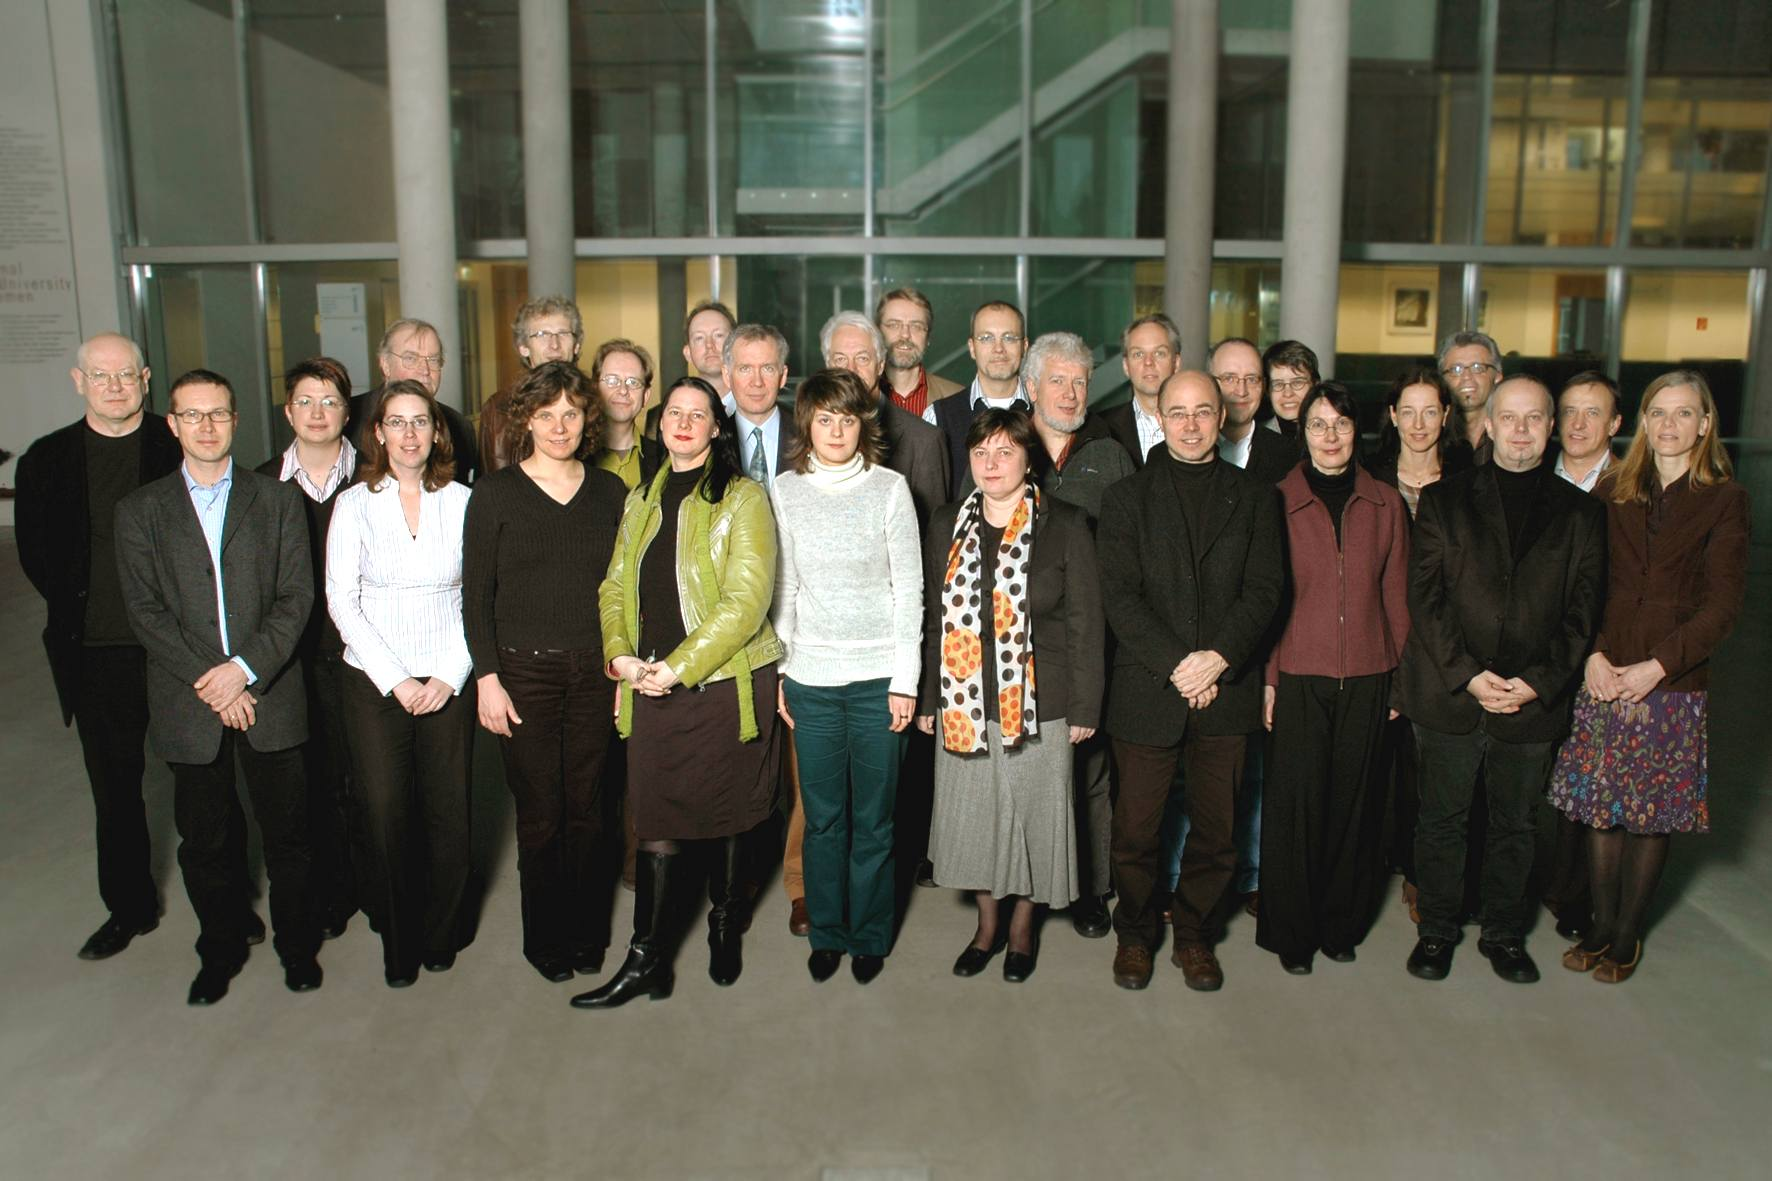
\includegraphics[width=1.00\textwidth]{Faculty1.jpg}
    
		\caption{}%\label{fig:profxxx}
   \end{center}
\end{figure}\\

December 2006


\newpage
\pagenumbering{Roman}
\thispagestyle{empty}
\begin{}
  \begin{center}
    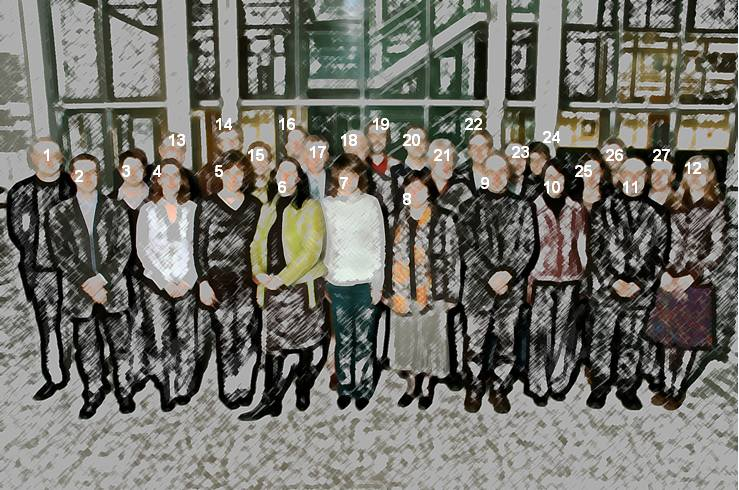
\includegraphics[width=1.00\textwidth]{Faculty2.jpg}
    
		\caption{}%\label{fig:profxxx}
   \end{center}
\end{figure}\\

\vskip 40

\begin{center}
\begin{quote}
\begin{tabular}{ll}
$\ \ \ \ $1$\ \ \ \ $ Paul Crowther $\ \ \ \ \ \ \ \ \ \ \ \ \ \ \ \ \ \ \ \ \ \ \ \ \ \ \ \ \ \ \ \ \ \ \ \ \ \ \ \ \ \ \ \ \ \ \ \ \ \ \ \ $ & 15$\ \ \ \ $ Gert Brunekreeft\\
$\ \ \ \ $2$\ \ \ \ $ Marc Frey & 16$\ \ \ \ $ Matthijs Bogaards\\
$\ \ \ \ $3$\ \ \ \ $ Bianca Bergmann & 17$\ \ \ \ $ Brendan Dooley\\
$\ \ \ \ $4$\ \ \ \ $ Claire Freeman & 18$\ \ \ \ $ Hendrik Birus (Dean)\\
$\ \ \ \ $5$\ \ \ \ $ Bettina Olk & 19$\ \ \ \ $ Hartmut Wessler\\
$\ \ \ \ $6$\ \ \ \ $ Marion G. M�ller & 20$\ \ \ \ $ Christian Welzel\\
$\ \ \ \ $7$\ \ \ \ $ Rena Dickel & 21$\ \ \ \ $ Klaus Boehnke\\
$\ \ \ \ $8$\ \ \ \ $ Immacolata Amodeo & 22$\ \ \ \ $ Ulrich K�hnen\\
$\ \ \ \ $9$\ \ \ \ $ Thomas Rommel & 23$\ \ \ \ $ Welf Werner \\
$\ \ \ \ $10$\ \ \ $ Margrit Schreier & 24$\ \ \ \ $ Nicola Spakowski \\
$\ \ \ \ $11$\ \ \ $ Arvid Kappas & 25$\ \ \ \ $ Freia Hardt \\
$\ \ \ \ $12$\ \ \ $ Hilke Brockmann & 26$\ \ \ \ $ Harald Fischer-Tin\'{e} \\
$\ \ \ \ $13$\ \ \ $ Georg Ress & 27$\ \ \ \ $ Peter Ludes \\
$\ \ \ \ $14$\ \ \ $ Adalbert FX Wilhelm&  $\ \ \ \ $   \\

\end{tabular}
\end{quote}
\end{center}


\vskip 30
{\bf Not in the picture}: Andreas Bausch, Jan Delhey, Adele Diederich, Jens F�rster, Ursula Frohne, Philipp Genschel, Kristine Hermann, Markus Jachtenfuchs, Debora Jeske, Christian Joppke, Petra Lietz, Johannes Paulmann, Susanne Peters, Wolfgang Pfaffenberger, Dirk Schulte am H�lse, Uwe Spiekermann, Jens Steffek, Michael Talias, Isabel W�nsche



\newpage
\fchapter{}
\thispagestyle{empty}
%\begin{titlepage}
\vfil\null
\begin{center}
\bigskip \bigskip \bigskip
\vspace{1.0in}
\large
\bigskip \bigskip
\end{center} 
\normalsize
\vfil\null
%\end{titlepage}




\onecolumn
 \cleardoublepage
 \shorttitle{Table of Contents} 
 \textbf{ }\vspace{-1cm}
 \tableofcontents

\ \\\
  \ \ \ \ \vspace*{8cm}\ \ \\ \vspace*{4cm}



\clearpage


\resetpages
	
\newpage
\shorttitle{Preface}
  \resetpages
 


\vspace*{3cm}
\begin{center}
\section*{Preface}
\addcontentsline{toc}{section}{Preface}
\end{center}
\vspace*{1cm}


In the summer of 2006 I took over, from my predecessor Max Kaase, the position of the Dean of Humanities and Social Sciences. I am very much impressed by the productivity and engagement in research shown by the members of the School and documented in this report.

\vspace*{7cm}





Bremen, November 2006	

Prof. Dr. Hendrik Birus \\
Dean of Humanities and Social Sciences



\newpage
\fchapter{}
\thispagestyle{empty}
%\begin{titlepage}
\vfil\null
\begin{center}
\bigskip \bigskip \bigskip
\vspace{1.0in}
\large
\bigskip \bigskip
\end{center} 
\normalsize
\vfil\null
%\end{titlepage}

\newpage
\shorttitle{Introduction}

\newpage
\section{Introduction}
For the third time, the School of Humanities and Social Sciences at IUB documents its research activities for interested parties inside and outside of the university. This report for one speaks to the broad variety of research concerns by the disciplines. At the same time, it also testifies to the growing engagement of faculty in collaborative work on common research topics and the international orientation of the School.
\\[-0.25cm]

By the end of 2006, the School has grown to the number of faculty which was foreseen in the initial IUB planning documents of 2000: about 34 professorships and one lecturer.
\\[-0.25cm]

The high quality of faculty recruited into the School has had its payoffs in its recognition by research funding agencies, the number and quality of publications and a broad variety of outside requests for involvement in scholarly and academic activities. But excellence also has its price as signalled by the considerable number of offers to faculty for posts at other universities, some of which were declined while others were accepted. Clearly one can look at this with the perspective of a half-full or a half-empty glass. In such fluctuation, however, there are also embedded disruptive tendencies, which may affect not only teaching, but also research.
\\[-0.25cm]

The humanities and to a lesser extent also the social sciences follow a different research logic than do the sciences. In general, in the former fields, research is much more individualized, often requires less infrastructure and is less collaborative nationally as well as internationally. However, at this School from the beginning research-as is true for teaching-has had strong empirical and methodological underpinnings and, wherever theoretically called for, places a lot of emphasis on cross-national and cross-cultural approaches. This is clearly visible in the research profile of the School and its faculty.
\\[-0.25cm]

Faculty members as individual researchers in the last years have been very successful in finding third-party financial support for their work especially from the Deutsche Forschungsgemeinschaft (DFG). But the School has also been successful in collaborative research, as is shown by the fact that two faculty members continue to direct a project each in the DFG-funded Collaborative Research Center (Sonderforschungsbereich) and that, jointly with the Universit�t Bremen, ISS and Methods faculty-even though in the first wave they did not succeed-has at least jumped the first hurdle for a Graduate School (Graduiertenschule) in the Social Sciences (Bremen International Graduate School of Social Sciences - $^{\rm\bf BI}${\itshape GSSS}) in the context of the Exzellenzinitiative and will re-apply for the second wave in 2007.







\cleardoublepage \onecolumn




\newpage
\fchapter{}
\thispagestyle{empty}
%\begin{titlepage}
\vfil\null
\begin{center}
\bigskip \bigskip \bigskip
\vspace{1.0in}
\large
\bigskip \bigskip
\end{center} 
\normalsize
\vfil\null
%\end{titlepage}

\newpage
\section{Art and Literature}
\shorttitle{Art and Literature}

\subsection{Prof. Dr. Immacolata Amodeo}


\textbf{Main Research Interests}\\[-0.25cm]
\begin{enumerate}
\item[$\bullet$]	Comparative Literature
\item[$\bullet$]	Comparative Media Studies
\item[$\bullet$]	Literary and Cultural Theory
\item[$\bullet$]	Intercultural and Transcultural Studies
\item[$\bullet$]	Literature in its Relations to other Media (mainly Opera, Music, and Film)
\item[$\bullet$]	Multilingualism and Literature
\item[$\bullet$]	Migration Literatures
\item[$\bullet$]	Aesthetic Aspects of Cultural Conflicts and Cultural Encounters
\end{enumerate}

\vspace{0.6cm}
\textbf{Research Activities}\\[-0.25cm]

Immacolata Amodeo has continued and diversified her research activities in the field of migrant literatures: (a) she worked on gender-related questions and literary texts written by migrant women writers of Italian origin in Germany; (b)  she studied the works of migrant writers with Spanish as first language (in the Federal Republic of Germany and the GDR); (c) she has further developed the comparative study of migrant literatures; d) she has analyzed linguistic aspects of migrant literatures. The analysis of linguistic aspects of migrant literatures led to the organization and establishment of an international and interdisciplinary research group (scholars from Germany, Italy, France and several African countries are involved) under her direction and a joint grant application with a research proposal on multilingualism and migrant literatures in Germany, Italy, and Canada from a comparative perspective (VolkswagenStiftung, program \textit{Studiengruppen zu Migration und Integration}, decision pending). Furthermore, she has started translating (from German into Italian) a collection of short-stories by the author of Italian origin Franco Biondi living in Germany and writing in German which she is committed to editing for publication in Italy in 2007. Immacolata Amodeo has also refined her analysis of political and cultural mappings of criminality and nationality in traditional and new media. This research (in collaboration with Eva Erdman, Universit�t Erfurt) lead to the idea of an online atlas of crime fiction and to data collection on the basis of contemporary crime novels. 


\vspace{0.6cm}
\textbf{Organization of Scientific Conferences}\\[-0.25cm]
\begin{enumerate}

\item[$\bullet$] March 2006\newline
 International University Bremen\newline
"Contemporary Indian Literature Conference"\newline (organized together with IUB students Annika Carlson, Cristina Galusca, Christin H�ne, Saskia Schirmann)\newline
funded by the Indian Embassy in Germany\newline
international participants: 40
\end{enumerate}



 

\vspace{0.6cm}
\textbf{Other Professional Activities}\\[-0.25cm]
\begin{enumerate}
\item[$\bullet$]	Committee work and reviewing for foundations and other institutions (the accreditation agency ACQUIN, the Alexander von Humboldt Foundation, the Studienstiftung des Deutschen Volkes, DAAD etc.)
\item[$\bullet$]	Member of the jury for the International Literature Prize \textit{Albatros} of the G�nter Grass-Stiftung Bremen
\item[$\bullet$]	Member of INPUTS (Institut f�r postkoloniale und transkulturelle Studien, Universit�t Bremen)
\item[$\bullet$]  Member of the advisory board of the exhibition \textit{Annelino. Zur Geschichte der Italiener in Ludwigshafen}, Kultur-Rhein-Neckar e.V. in collaboration with the Stadtmuseum Ludwigshafen (December 2005-March 2006)
\item[$\bullet$]  Moderation of the round table discussion with the authors Silvia Di Natale, Marisa Fenoglio, Lisa Mazzi, Venera Tirreno Schneider, Istituto Italiano di Cultura di Francoforte / Coordinamento Donne Francoforte, Frankfurt am Main, 17 March 2006
\item[$\bullet$]  Coordinator (together with Prof. Dr. Nicola Spakowski) of the Humanities Graduate Program \textit{Intercultural Humanities}, International University Bremen
\item[$\bullet$]  External PhD examiner University of Bayreuth, Germany

\end{enumerate}


\vspace{0.6cm}
\textbf{PhD-Students}\\[-0.25cm]

Irina Chkhaidze \newline
\textit{Posthuman Bodies: Conceptualising Hybrids}\\[-0.15cm]

Heidrun Gudrun H�rner \newline
\textit{China's New Literature is Taking Place Abroad: How Authors of Chinese Origin in France and Germany Write - A Comparative Analysis}\\[-0.15cm]

Brigitte Kienle \newline
\textit{On "New World Literatures": Globalization, Migration and Aesthetics in the Literature of Migrant African Authors in Italy}\\[-0.15cm]

\newpage
\subsection{Prof. Dr. Paul Crowther}


\textbf{Main Research Interests}\\[-0.25cm]
\begin{enumerate}
\item[$\bullet$]	Philosophy of Art and Culture
\item[$\bullet$]	Meaning in the Visual Arts
\item[$\bullet$]  Hegelian and Phenomenological Logic and Metaphysics 
\item[$\bullet$]	Philosophy of Art History
\item[$\bullet$]  Victorian Art
\end{enumerate}


\vspace{0.6cm}
\textbf{Research Activities}\\[-0.25cm]

Paul Crowther has worked on three book projects during 2006. He has completed editing and critically introducing the book by R.K. Elliott, \textit{Aesthetics, Imagination, and the Unity of Experience}, which has meanwhile appeared with the Ashgate publishing house. A second book project was concerned with \textit{Defining Art, Creating the Canon: Artistic Value in an Era of Doubt}. It is being published by Oxford University Press. Paul Crowthers' most recent interest is directed towards the \textit{Phenomenology of the Visual Arts}; this book is under review with Cornell University Press. Furthermore Paul Crowther has co-organized a conference on {\itshape Art and Metaphysics}. The conference addressed both historical and conceptual aspects of the relation between visual art and metaphysics. In it the term "metaphysics" was understood broadly so as to encompass philosophical, religious, and scientific meaning. 
\vspace{0.6cm}


\textbf{Organization of Scientific Conferences}\\[-0.25cm]
\begin{enumerate}
\item[$\bullet$]	May 2006\newline
	International University Bremen\newline
  "Art and Metaphysics in the Twentieth Century and Beyond"\newline
	(together with Prof. Dr. Isabel W�nsche \& Prof. Dr. Ursula Frohne, IUB)\newline
  funded by the DFG\newline
  international participants: 75
\end{enumerate}


\vspace{0.6cm}
\textbf{Other Professional Activities}\\[-0.25cm]
\begin{enumerate}
\item[$\bullet$] Visiting Fellow at the Slovene Academy of Arts and Sciences
\end{enumerate}


\newpage
\subsection[Prof. Dr. Ursula Anna Frohne] {Prof. Dr. Ursula Anna Frohne {\normalfont\normalsize\newline(Left IUB in March 2006)}}
 


\textbf{Main Research Interests}\\[-0.25cm]
\begin{enumerate}
\item[$\bullet$]	$19^{\rm th} - 21^{\rm st}$ Centuries Art (American and European Art, Self-Referentiality, Art in Public Space, Ephemeral Art Practices, Exhibition History)
\item[$\bullet$]	New Media (Photography, Film, Video, Electronic Media, Multi-Media Installations and Media Transcriptions)
\item[$\bullet$]  Science of the Image (Visual Culture and Cultural Techniques)
\item[$\bullet$]	Art and Politics (Politics and Ethics of Visibility, Art and Agency, Iconicity of Social Reality)
\item[$\bullet$]  Art Market Phenomena and Value Transformations in Art
\end{enumerate}


\vspace{0.6cm}
\textbf{Research Activities}\\[-0.25cm]

Ursula Frohne's longstanding project addresses self-referential practices in art since the mid-$20^{\rm th}$ century. The book emerging from this work explores the conceptual dimensions of diverse appropriative artistic methods and their inter-medial transcriptions. It theorizes the aesthetic and cultural significance of mimetic repetition, recycling, copying, and re-staging of visual material in the field of art and the role of new media technologies in this. A second project is dedicated to the investigation of reflections of filmic space, particularly in contemporary media installations, consisting of illusionary spatial projections with extensions into the exhibition space. It is based on a collaborative research initiative between the Art History Department of the Universit�t Frankfurt am Main and the Media Studies Department of the Universit�t Jena; an application for DFG-funding has been submitted in June 2006. In the context of the Graduiertenkolleg \textit{Bild - K\"{o}rper - Medium. Eine anthropologische Perspektive} at the Staatliche Hochschule f\"{u}r Gestaltung Karlsruhe to which Ursula Frohne is affiliated as an external professor since 2003, she has dedicated her research to image theory, visual culture and politics. Questions concerning visual representations of social reality, ethics and politics of visibility, the potential of images to initiate agency and intercultural dimensions of image transfers are of major interest in this context. Another project is based on a research collaboration with the Neues Museum Weserburg Bremen. Its preliminary investigations of collaborative structures and process-based concepts in the field of art since the 1960s will be materializing in a grant application to further historically contextualize and reconstruct ephemeral art tendencies. Finally Ursula Frohne is dedicated to the investigation of significant shifts in the value system of the modern and contemporary art market, entailing the relation between the aesthetic and the economic value of the art work. Special emphasis is given to the value producing systems (price politics of galleries, auction houses and the role of annual art fairs for the international art market, Corporate Collecting, etc.) and the emergence of new art markets in zones of political transformation. 

\vspace{0.6cm}


\textbf{Funded Projects}\\[-0.25cm]
\begin{enumerate}
\item[$\bullet$]   Participation in the collaborative grant application for the Graduiertenkolleg \textit{Bild - K\"{o}rper - Medium. Eine anthropologische Perspektive} at the Staatliche Hochschule f\"{u}r Gestaltung Karlsruhe concerning the third funding phase 2006 - 2009.\newline
 DFG-funding was granted in August 2006.
\end{enumerate}


\vspace{0.6cm}
\textbf{Organization of Scientific Conferences}\\[-0.25cm]
\begin{enumerate}
\item[$\bullet$]	May 2006\newline
	International University Bremen\newline
  "Art and Metaphysics in the Twentieth Century and Beyond"\newline
  (together with Prof. Dr. Paul Crowther \& Prof. Dr. Isabel W�nsche, IUB)\newpage
	funded by the DFG\newline
	international participants: 75
\item[$\bullet$]	July 2006\newline
	Universit\"{a}t Karlsruhe\newline
	"Politische Kunst - Politik der Kunst"\newline
	(in collaboration with Prof. Dr. Jutta Held)\newline
	funded by the Universit�t Karlsruhe and the Guernica Gesellschaft\newline
	international participants: 50
\end{enumerate}


\vspace{0.6cm}
\textbf{Other Professional Activities}\\[-0.25cm]
\begin{enumerate}
\item[$\bullet$] Editorial Board Member of the book series \textit{Interfaces. Studies in Visual Culture}, University of New England Press (Editors: Prof. Dr. Adrian Randolph und Prof. Dr. Mark J. Williams)
\item[$\bullet$] Editorial Board Member of the electronic journal \textit{Vectors: Culture and Technology in a Dynamic Vernacular}, University of Southern California
\item[$\bullet$] Member of the Scientific Board of the Research Association of the Archive for Small Press \& Communication / ASPC, Neues Museum Weserburg, Bremen
\item[$\bullet$] Selection Committee Member at the Fulbright Foundation
\item[$\bullet$] Member of the Board of the Haus im Park at the Klinikum Bremen-Ost
\item[$\bullet$] Member of the Editorial Board of the Jahrbuch des Wallraf-Richartz-Museum and Museum Ludwig, K\"oln
\item[$\bullet$] Member of the Lehrekommission at the Universit\"{a}t K\"{o}ln
\item[$\bullet$] Member of the Exzellenzclusterinitiative \textit{Media: Material Conditions and Cultural Practice} at the Universit\"{a}t K\"{o}ln
\item[$\bullet$] Member of the committee for the development of a concept for a Graduate School \textit{Wissen - Rezeption - Transkulturalit\"{a}t} at the University of Cologne under the thematic focus "Medialit\"{a}t[en]: Prozesse der Formierung und Transformation"
\item[$\bullet$] Member of the Scientific Board of conferences organized within the Graduiertenkolleg "Bild - K\"{o}rper - Medium", Staatliche Hochschule f�r Gestaltung Karlsruhe
\end{enumerate}




\vspace{0.6cm}
\textbf{PhD-Students}\\[-0.25cm]


Julia Bannenberg\newline
\textit{"Deutschlandbilder": Ein deutsch-deutsches Ausstellungskonzept}\\[-0.15cm]

Kirsten Fitzke\newline
\textit{Lebende Denkm\"{a}ler: Darstellungen kriegsversehrter K\"{o}rper im 20. Jahrhundert}\\[-0.15cm]

Sophie Gerlach\newline
\textit{Neo Rauch - Bilder 1984 - 2005. Maler und Werk als Projektionsfl\"{a}che gesellschaftspolitischer Tendenzen}\\[-0.15cm]

Katja Hoffmann\newline
\textit{Zur Relevanz des 'iconic turn' in der Kunstwissenschaft: \"{U}berlegungen zur Ph\"{a}nomenologie, Theorie und Historiografie eines Paradigmas - am Beispiel der Documenta 11 (2002) und der Ausstellung Film und Fotografie (1929)}\\[-0.15cm]

Charlotte Kraft\newline
\textit{Rosemarie Trockel: Identit\"{a}ten}\\[-0.15cm]

Sebastian Neusser\newline
\textit{Die submediale Pr�senz des K�rpers in der Kunst}\\[-0.15cm]

\newpage
Stefanie Zobel\newline
\textit{(Working title) Zeitgen�ssische (Re)Pr\"{a}sentation von Medienkunst: Ausstellungskonzepte und -formate}\\[-0.15cm]

Doroth\'{e}e Brill\newline
\textit{Shock of the Void. The Senseless as Strategy in Dada and Fluxus}


\vspace{0.6cm}
\textbf{Research Personnel}\\[-0.25cm]

Katja Hoffmann \newline Research Associate
\newpage
\subsection[PD Dr. Susanne Peters] {PD Dr. Susanne Peters {\normalfont\normalsize\newline (Visiting Professor in Fall 2006)}}


\textbf{Main Research Interests}\\[-0.25cm]
\begin{enumerate}
\item[$\bullet$]	Sense Perception in Literature
\item[$\bullet$]	Orality and Literacy
\item[$\bullet$]	Intercultural Communication
\item[$\bullet$]	Intermediality
\item[$\bullet$]	History and Theory of Drama and Theatre
\item[$\bullet$]	Censorship
\end{enumerate}


\vspace{0.6cm}
\textbf{Research Activities}\\[-0.25cm]

After her habilitation with a major study on the role and function of letters in drama from the $16^{\rm th}$ century to the present, Susanne Peters has focused her research on the relationship between oral and written discourse in fiction and drama and the creation and distortion of public and private spheres in literature. She also continued to enquire into the role of sense perception in literature as well as film that she started with her dissertation on the works of James Joyce. Further areas of research were intercultural communication with a special interest in intercultural incompetence, and literatures from English-speaking countries. With two colleagues she has recently founded and co-edits a new series of scholarly books on teaching contemporary literature and culture, of which the first volume in two parts, offering readings of 31 plays, has just been published. The series presents accessible readings of major works of contemporary literature in English for schools and universities, with an emphasis on teachability. The next volume, again in two parts, dealing with the teaching of novels, is currently in preparation and will appear in 2007. Susanne Peters has held visiting professorships at the universities of Leipzig, D�sseldorf, and Stuttgart. She joined IUB in spring 2006 as lecturer and is currently visiting professor.
\vspace{0.6cm}

\textbf{Other Professional Activities}\\[-0.25cm]
\begin{enumerate}
\item[$\bullet$] Member of Deutscher Anglistenverband
\item[$\bullet$] Member of Deutsche Shakespeare-Gesellschaft
\item[$\bullet$] Member of Deutsch-Britische Gesellschaft
\item[$\bullet$] Member of Gesellschaft f�r die Neuen Englischsprachigen Literaturen (GNEL/ASNEL)
\item[$\bullet$] Member of The German Society for Contemporary Drama and Theatre in English (CDE)
\end{enumerate}

\newpage
\subsection{Prof. Dr. Thomas Rommel }

\textbf{Main Research Interests}\\[-0.25cm]
\begin{enumerate}
\item[$\bullet$]	18th-Century Literature
\item[$\bullet$]	Romanticism
\item[$\bullet$]	Humanities Computing
\item[$\bullet$]	Literature, Moral Philosophy and Economics
\item[$\bullet$]	Literary Theory
\end{enumerate}


\vspace{0.6cm}
\textbf{Research Activities}\\[-0.25cm]

Thomas Rommel received his doctorate and habilitation in Literary Studies at the University of T\"{u}bingen. His previous positions include Northern Arizona University, Columbia University, New York, and Joensuu University, Finland. He is co-editor of the online journal \textit{Prolepsis} and he is on the board of the Association for Literary and Linguistic Computing, ALLC. His research interests include Romanticism with a book on Lord Byron, a study of 18th-century literature and the history of ideas, and a book on Adam Smith. He has written an introduction to academic work for students of literature, and he edited several conference volumes. He is currently editing two more books on \textit{Transculturality in the Diaspora and The Fable of the Market. The Convergence of Literary, Economic, and Historical Discourses, 1700-1850}, together Paul Nolte, to be published by Francke Verlag, T\"{u}bingen. In addition, Rommel writes a regular column in a Bremen newspaper on literature. This column is addressed to non-academic readers, and so far two volumes have appeared: \textit{Literaturspalten}, on general questions of literature, and \textit{50 Klassiker der Weltliteratur}, on canonical literature.
\begin{figure}[ht]
  \begin{center}
    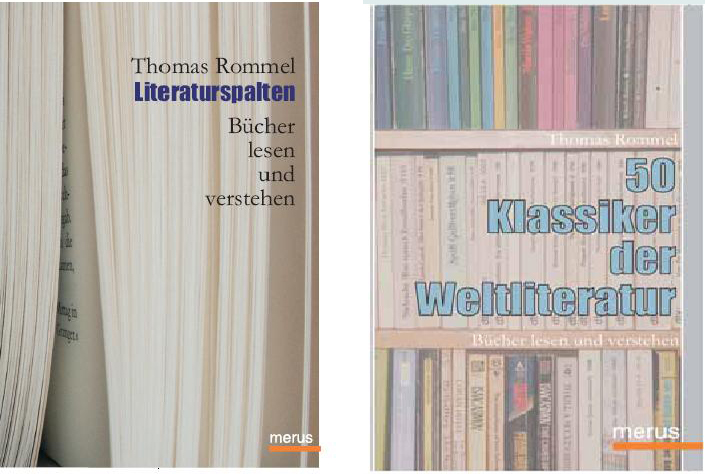
\includegraphics[width=0.8\textwidth]{./ArtLit/Rommel.jpg}
%   \mycaption{ xxx )}\label{fig:profxxx}
   \end{center}
\end{figure}






\vspace{0.6cm}
\textbf{Other Professional Activities}\\[-0.25cm]
\begin{enumerate}
\item[$\bullet$] Member of the Executive Committee of ALLC (Association for Literary and Linguistic Computing)
\item[$\bullet$] Member of INPUTS, Institut f�r postkoloniale und transkulturelle Studien, Universit�t Bremen
\item[$\bullet$] Co-editor of \textit{Prolepsis, the Heidelberg Review of English Studies.} With Richard Utz (University of Northern Iowa), Peter Paul Schnierer (Universit\"{a}t Heidelberg)
\item[$\bullet$] Vertrauensdozent, Studienstiftung des Deutschen Volkes
\item[$\bullet$] Board Member of Bremen Brain; Bremen Brain provides Bremen's scientists with a forum for interdisciplinary discussions and lectures. The aim is to improve Bremen's image and to organize different conferences using the contacts of BB-Members
\end{enumerate}




\vspace{0.6cm}
\textbf{PhD-Students}\\[-0.25cm]

Cansu \"{O}zmen\newline
\textit{American Travel Narratives in the 19th Century}\\[-0.15cm]

Mark Schreiber\newline
\textit{The Celtic Tiger on Stage and Screen. An Analysis of Contemporary Irish Theatre}\\[-0.15cm]

Beril Saydun\newline
\textit{Constructing Turkish Nationalism and Autobiographic Selves in Halide Edib's Works "Memoirs of Halide Edib, The Turkish Ordeal and Inside India"}\\[-0.15cm]

Susanne Puissant\newline
\textit{Irony and Satire in the Poetry of the First World War}\\[-0.15cm]
\newpage
\subsection{Prof. Dr. Isabel W\"{u}nsche}


\textbf{Main Research Interests}\\[-0.25cm]
\begin{enumerate}
\item[$\bullet$]	$19^{\rm th}$ and $20^{\rm th}$-Century Art and Art Theory
\item[$\bullet$]	European and American Modernism
\item[$\bullet$]	The European Avant-Garde Movements
\item[$\bullet$]	The Organic School of the Russian Avant-Garde
\item[$\bullet$]	Abstraction in Art
\item[$\bullet$]	Interrelations between Art and Science
\item[$\bullet$]	Biocentrism
\item[$\bullet$]	Synesthesia
\item[$\bullet$]	The Transatlantic Dialogue
\end{enumerate}


\vspace{0.6cm}
\textbf{Research Activities}\\[-0.25cm]

The main focus of Isabel W\"{u}nsche's work in early 2006 was the completion of her study on and the publication of the selected correspondence between Galka E. Scheyer, American representative of the Blue Four, and the Blue Four artists Lyonel Feininger, Alexej von Jawlensky, Wassily Kandinsky, and Paul Klee. Published in an English-language as well as a German-language edition by Benteli, Berne, in spring 2006, the extensively annotated correspondence focuses on the transatlantic, artistic dialogue and the introduction of European modernism to the United States. Isabel W\"{u}nsche has continued to cover the following areas: (a) organic abstraction, biocentric modernism, and the influence of the life sciences upon modernist art and design during the period 1890-1960 (various papers, major contribution to an exhibition catalogue, book chapters, preparation of an anthology with University of Pittsburgh Press); (b) ongoing work concerning the Organic School of the Russian avant-garde (various papers, book publication plans with UK publisher); (c) an extended study of the Leningrad Sterligov School that pursued abstraction in the spirit of the avant-garde during the period 1960-1990 (various papers, exhibition project at Rutgers University to be concluded in 2007). A new research project on \textit{European Modernism: Cultural Identities between National Presentation and International Orientation} was initiated with a symposium on the contribution of Russian art to European modernism in August 2006 and is currently being developed into a collaborative research project with an international team of colleagues.
\begin{figure}[ht]
  \begin{center}
    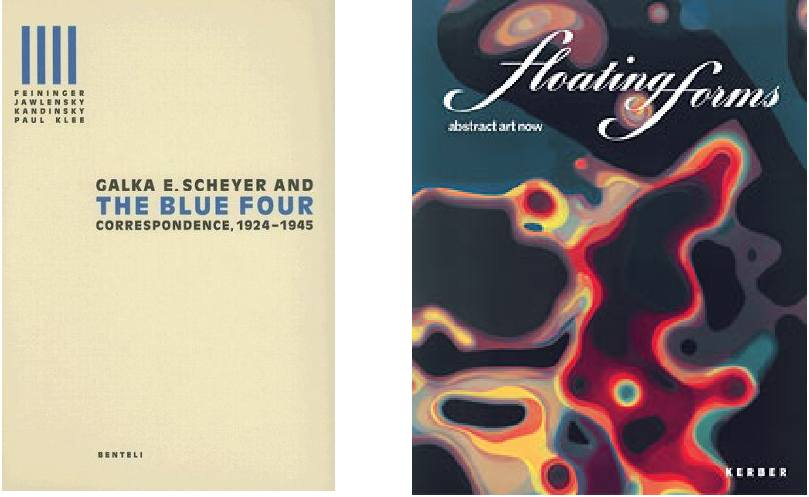
\includegraphics[width=0.85\textwidth]{./ArtLit/Wuensche.jpg}
%   \mycaption{ xxx )}\label{fig:profxxx}
   \end{center}
\end{figure}

\vspace{0.6cm}


\textbf{Funded Projects}\\[-0.25cm]
\begin{enumerate}
\item[$\bullet$]   Research Project: \textit{Der Beitrag der russischen Kunst zur europ�ischen Moderne}, funded by the Karin und Uwe Hollweg Stiftung, Bremen (research, symposium, publication)
\item[$\bullet$]   Exhibition Project: \textit{The Heritage of the Russian Avant-Garde: Vladimir Sterligov and his School}, from the Nancy and Norton Dodge Collection of Nonconformist Art from the Soviet Union at Rutgers, The State University of New Jersey, New Brunswick, funded by the Nancy and Norton Dodge Foundation
\end{enumerate}






\vspace{0.6cm}
\textbf{Organization of Scientific Conferences}\\[-0.25cm]
\begin{enumerate}
\item[$\bullet$]May 2006\newline
International University Bremen\newline
"Art and Metaphysics in the Twentieth Century and Beyond"\newline
(together with Prof. Dr. Paul Crowther \& Prof. Dr. Ursula Frohne, IUB)\newline
funded by the DFG\newline
international participants: 75
\item[$\bullet$]August 2006\newline
International University Bremen\newline
"Ferne \& N\"{a}he: Der Beitrag der russischen Kunst zur europ\"{a}ischen Moderne"\newline
(together with PD Dr. Ada Raev, Humboldt-Universit\"{a}t Berlin)\newline
funded by the Karin und Uwe Hollweg Stiftung, Bremen\newline
international participants: 50
\end{enumerate}



\vspace{0.6cm}
\textbf{Other Professional Activities}\\[-0.25cm]
\begin{enumerate}
\item[$\bullet$] Organization of a Workshop on the Nature of Abstraction in European Modernism, IUB, October 2006
\item[$\bullet$] Organization of the Conference Panel: "The Idea of Evolution in Literature and Art: How Darwin Shaped Literary Theory and Modernist Art History Writing," 20th Annual Conference of the Society of Literature, Science, and the Arts (SLSA), Dactyl Foundation, New York, November 2006
\end{enumerate}







\vspace{0.6cm}
\textbf{PhD-Students}\\[-0.25cm]

Isabelle Schwarz\newline
\textit{Archive f\"{u}r K\"{u}nstlerpublikationenen der 1960er bis 1980er Jahre}\newline
(Archives of Artists' Publications from the 1960s to the 1980s)\newline
Defense: May 2006\\[-0.15cm]

Yuliya Salauyova\newline
\textit{Walter Benjamin on Montage and Soviet Cinema: Historical and Theoretical Aspects of the "Politicization of Aesthetics"}\\[-0.15cm]

Laura Petican\newline
\textit{The Persistence of a Baroque Mentality in Arte Povera}\\[-0.15cm]

Carin Baban\newline
\textit{Image Appropriation in 20th-Century Art}\\[-0.15cm]


\vspace{0.6cm}
\textbf{Research Personnel}\\[-0.25cm]

Elina Knorpp, M.A.

\newpage
%Publications for History

%the function for the book publication could be as follows [it was not implemented here]
%1=author;2=year;3=title;4=publisher + comments
%\newcommand{\book}[4]{#1 (#2). \textit{#3}. #4}

\newpage

\subsection{Publications}




	\paragraph{Books} \textit{ }
	
\bigskip	


Dooley, B. (Ed.) (2006). \textit{Energy and culture: Perspectives on the power to work}. Burlington, VT: Ashgate. \\ 

Fischer-Tin\'{e}, H. (2006). \textit{Ausnahmezustand}. Novel by Nirmal Verma, translated from Hindi by H. Fischer-Tin\'{e}, \& H. Bauhaus-L\"{o}tzke. Heidelberg: Draupadi.\\ 

Frey, M. (2006). \textit{Dekolonisierung in S\"{u}dostasien. Die Vereinigten Staaten und die Aufl\"{o}sung der europ\"{a}ischen Kolonialreiche}. M\"{u}nchen: Oldenbourg.\\ 

Leutner, M., Spakowski, N., \& Yu, C.M. (Eds.) (2006). \textit{Gonghe shidai de Zhongguo fun\"{u} (Women in China. The Republican Period in Historical Perspective)}. Taipei: Rive Gauche Publishing, in press.\\ 

Paulmann, J. (2006). \textit{Die Haltung der Zur\"{u}ckhaltung: Ausw\"{a}rtige Selbstdarstellungen nach 1945 und die Suche nach einem erneuerten Selbst-verst\"{a}ndnis in der Bundesrepublik} (= Schriftenreihe der Wilhelm und Helene Kaisen-Stiftung), Bremen: Kaisen-Stiftung.\\ 

Spakowski, N., \& Milwertz, C. (Eds.) (2006). \textit{Women and gender in Chinese Studies. Special issue of Chinese History and Society/Berliner China-Hefte}, 29.\\ 



\paragraph{Articles \& Chapters}\textit{ }

\bigskip


Dooley, B. (2006). Art and information brokerage in the career of Don Giovanni de' Medici. In H. Cools, M. Keblusek, \& B. Noldus (Eds.), \textit{Your Humble Servant} (pp. 81-96). Hilversum: Verloren.\\ 

Fischer-Tin\'{e}, H. (2006). Global civil society and the forces of empire. The Salvation Army, British imperialism and the "pre-history" of NGOs. In S. Conrad, \& D. Sachsenmaier (Eds.), \textit{Conceptions of world order: Global historical approaches} (pp. 25-57). New York: Palgrave, in press.\\ 

Fischer-Tin\'{e}, H. (2006). Stadt der Pal\"{a}ste? - Europ\"{a}ische Lebenswelten im kolonialen Kalkutta. In R. Ahuja, \& C. Brosius (Eds.), \textit{Megast\"{a}dte in Indien: Mumbai, Delhi, Calcutta} (pp. 241-256). Heidelberg: Draupadi. \\ 

Fischer-Tin\'{e}, H. (2006). "Deep Occidentalism"? - Europa und der Westen in der Wahrnehmung hinduistischer Intellektueller und Reformer (ca. 1890-1930). \textit{Journal of Modern European History, 4}(2), 171-203.\\ 

Fischer-Tin\'{e}, H. (2006). From \textit{Brahmacharya} to conscious race culture: Indian nationalism, Hindu tradition and Victorian discourses of science. In C. Bates (Ed.), \textit{Beyond representation. The construction of identity in colonial India }(pp. 230-59). New Delhi: Oxford University Press.\\ 

Fischer-Tin\'{e}, H. (2006). Ananda Marga. In C. Auffahrt, H.-G. Kippenberg, \& A. Michaels (Eds.), \textit{W\"{o}rterbuch der Religionen }(p. 32). Stuttgart: Kr\"{o}ner.\\ 

Fischer-Tin\'{e}, H. (2006). Arya Samaj. In C. Auffahrt, H.-G. Kippenberg, \& A. Michaels (Eds.), \textit{W\"{o}rterbuch der Religionen }(p. 45). Stuttgart: Kr\"{o}ner.\\ 

Fischer-Tin\'{e}, H. (2006). Brahmo Samaj. In C. Auffahrt, H.-G. Kippenberg, \& A. Michaels (Eds.), \textit{W\"{o}rterbuch der Religionen }(p. 80). Stuttgart: Kr\"{o}ner.\\ 

Fischer-Tin\'{e}, H. (2006). Dayanand Sarasvati. In C. Auffahrt, H.-G. Kippenberg, \& A. Michaels (Eds.), \textit{W\"{o}rterbuch der Religionen }(p. 103). Stuttgart: Kr\"{o}ner.\\ 

Fischer-Tin\'{e}, H. (2006). Keshab Chandra Sen. In C. Auffahrt, H.-G. Kippenberg, \& A. Michaels (Eds.), \textit{W\"{o}rterbuch der Religionen} (p. 280). Stuttgart: Kr\"{o}ner.\\ 

Fischer-Tin\'{e}, H. (2006). Krishnamurti. In C. Auffahrt, H.-G. Kippenberg, \& A. Michaels (Eds.), \textit{W\"{o}rterbuch der Religionen} (p. 296). Stuttgart: Kr\"{o}ner.\\ 

Fischer-Tin\'{e}, H. (2006). Maharishi Mahesh Yogi. In C. Auffahrt, H.-G. Kippenberg, \& A. Michaels (Eds.), \textit{W\"{o}rterbuch der Religionen} (p. 318). Stuttgart: Kr\"{o}ner.\\ 

Fischer-Tin\'{e}, H. (2006). Neohinduismus. In C. Auffahrt, H.-G. Kippenberg, \& A. Michaels (Eds.), \textit{W\"{o}rterbuch der Religionen} (pp. 370-371). Stuttgart: Kr\"{o}ner.\\ 

Fischer-Tin\'{e}, H. (2006). Radhakrishnan. In C. Auffahrt, H.-G. Kippenberg, \& A. Michaels (Eds.), \textit{W\"{o}rterbuch der Religionen} (p. 419). Stuttgart: Kr\"{o}ner.\\ 

Fischer-Tin\'{e}, H. (2006). Rajneesh. In C. Auffahrt, H.-G. Kippenberg, \& A. Michaels (Eds.), \textit{W\"{o}rterbuch der Religionen} (p. 419). Stuttgart: Kr\"{o}ner.\\ 

Fischer-Tin\'{e}, H. (2006). Ramana Maharshi. In C. Auffahrt, H.-G. Kippenberg, \& A. Michaels (Eds.), \textit{W\"{o}rterbuch der Religionen} (p. 420). Stuttgart: Kr\"{o}ner.\\ 

Fischer-Tin\'{e}, H. (2006). Sri Aurobindo. In C. Auffahrt, H.-G. Kippenberg, \& A. Michaels (Eds.), \textit{W\"{o}rterbuch der Religionen} (p. 496). Stuttgart: Kr\"{o}ner.\\ 

Fischer-Tin\'{e}, H. (2006). Sundar Singh. In C. Auffahrt, H.-G. Kippenberg, \& A. Michaels (Eds.), \textit{W\"{o}rterbuch der Religionen} (p. 504). Stuttgart: Kr\"{o}ner.\\ 

Fischer-Tin\'{e}, H. (2006). Tagore (Debendranath). In C. Auffahrt, H.-G. Kippenberg, \& A. Michaels (Eds.), \textit{W\"{o}rterbuch der Religionen} (p. 509). Stuttgart: Kr\"{o}ner.\\ 

Fischer-Tin\'{e}, H. (2006). Tagore (Rabindranath). In C. Auffahrt, H.-G. Kippenberg, \& A. Michaels (Eds.), \textit{W\"{o}rterbuch der Religionen} (p. 509). Stuttgart: Kr\"{o}ner.\\ 

Fischer-Tin\'{e}, H. (2006). Vivekananda. In C. Auffahrt, H.-G. Kippenberg, \& A. Michaels (Eds.), \textit{W\"{o}rterbuch der Religionen} (p. 558). Stuttgart: Kr\"{o}ner.\\ 

Frey, M. (2006). Die Vereinigten Staaten und die Dritte Welt w\"{a}hrend des Kalten Krieges. In B. Greiner, \& D. Walther (Eds.), \textit{Hei�e Kriege im Kalten Krieg} (pp. 27-56). Hamburg: Hamburger Edition. \\ 

Frey, M. (2006). Zivilgesellschaft in historischer Perspektive: Die Niederlande und Deutschland im 19. Jahrhundert. \textit{Zentrum f\"{u}r Niederlande-Studien Jahrbuch f\"{u}r 2005, 16}, 11-32.\\ 

Frey, M. (2006). Mao Zedong. Nationalist und Despot. In S. F\"{o}rster, \& M. P\"{o}hlmann (Eds.), \textit{Kriegsherren der Weltgeschichte. 22 Historische Portraits} (pp. 357-372). M\"{u}nchen: C.H. Beck.\\ 

Spakowski, N., \& Milwertz, C. (2006). Introduction: Women and gender in Chinese Studies and the Women and Gender in Chinese Studies Network (WAGNet). In N. Spakowski, \& C. Milwertz (Eds.), \textit{Women and Gender in Chinese Studies}. Special issue of \textit{Chinese History and Society/Berliner China-Hefte, 29}, 3-4.\\ 

Spiekermann, U. (2006). From neighbour to consumer. The transformation of retailer-consumer relationships in twentieth-century Germany. In F. Trentmann (Ed.), \textit{The making of the consumer. Knowledge, power and identity in the modern world} (pp. 147-174). Oxford: Berg.\\ 

Spiekermann, U. (2006). Warum scheitert Ern\"{a}hrungskommunikation? In Aid e.V. (Ed.), \textit{Ern\"{a}hrungskommunikation. Neue Wege - neue Chancen?}. (pp. 11-20). Bonn: Aid.\\ 

Spiekermann, U. (2006). Warum scheitert die Ern\"{a}hrungskommunikation? Eine Antwort aus kulturwissenschaftlicher Perspektive. In E. Barl\"{o}sius, \& R. Rehaag (Ed.), \textit{Anforderungen an eine \"{o}ffentliche Ern\"{a}hrungskommunikation} (pp. 39-51). Berlin: Wissenschaftszentrum.\\ 

Spiekermann, U. (2006). Warenwelten. Die Normierung der Nahrungsmittel in Deutschland 1880-1930. In R.-E. Mohrmann (Ed.), \textit{Essen und Trinken in der Moderne} (pp. 99-124). M\"{u}nster: Waxmann.\\ 

Spiekermann, U. (2006). Brown bread for victory: German and British wholemeal politics in the interwar period. In F. Trentmann, \& F. Just (Ed.), \textit{Food and conflict in Europe in the age of the two World Wars} (pp. 143-171). Basingstoke: Palgrave Macmillan.\\ 

\newpage
%Lecture Talks for Psychology

\newpage  
\subsection{Invited Scientific Lectures and Talks}

{\hyphenpenalty=5000
\begin{flushleft}
January 2006\\[0.5cm]
\end{flushleft}
\begin{tabular}{lp{13.4cm}}
 Speaker:	&   Jens F\"{o}rster \\
 Place: 	 & Palm Springs, CA, USA\\
 Event:   &	Meeting of the Society for Personality and Social Psychology (SPSP) \\
 Title: &	Catharsis Revisited: Inhibition of Aggression-Related Constructs after Goal-Fulfillment (with Markus Denzler and Nira Liberman) \\ \\
\end{tabular}
\begin{tabular}{lp{13.4cm}}
 Speaker:	&   Jens F\"{o}rster \\
 Place: 	 & Palm Springs, CA, USA\\
 Event:   &	Meeting of the Society for Personality and Social Psychology (SPSP) \\
 Title: &	Abstract and Concrete Thinking: The Effects of Motivational Cues on Thinking Styles (with Stefanie Kuschel) \\ \\
\end{tabular}
\begin{tabular}{lp{13.4cm}}
 Speaker:	&   Jens F\"{o}rster \\
 Place: 	 & Palm Springs, CA, USA\\
 Event:   &	7th Annual Meeting of the Society for Personality and Social Psychology (SPSP)\\
 Title: &	Regulatory Focus and the Evaluation of Visual Arts - Implications for Motivational Effects on Attitudes (with Katrin Schimmel)\\ \\
\end{tabular}
\begin{tabular}{lp{13.4cm}}
 Speaker:	&   Jens F\"{o}rster \\
 Place: 	 & Palm Springs, CA, USA\\
 Event:   &	7th Annual Meeting of the Society for Personality and Social Psychology (SPSP)\\
 Title: &	Novelty Theory\\ \\
\end{tabular}
\begin{tabular}{lp{13.4cm}}
 Speaker:	&   Jens F\"{o}rster \\
 Place: 	 & Columbia University, New York, NY, USA\\
 Event:   &	Guest lecture\\
 Title: &	Novelty Theory\\ \\
\end{tabular}
\begin{tabular}{lp{13.4cm}}
 Speaker:	&   Jens F\"{o}rster \\
 Place: 	 & Bremen\\
 Event:   &	Conference "Jazzahead"\\
 Title: &	Zwischen Chaos und Sicherheit: Jazz als Modell einer balancierten Organisation mit innovativem Charakter\\ \\
\end{tabular}
\begin{tabular}{lp{13.4cm}}
 Speaker:	&   Jens F\"{o}rster \\
 Place: 	 &Zentrum f\"{u}r feministische Studien, Universit\"{a}t Bremen\\
 Event:   &	Guest lecture\\
 Title: &	Zur Sozialpsychologie der Vorurteile\\ \\
\end{tabular}
\begin{tabular}{lp{13.4cm}}
 Speaker:	&  	Ulrich K\"{u}hnen \\
 Place: 	 &Palm Springs, CA, USA\\
 Event:   &	7th Annual Meeting of the Society for Personality and Social Psychology (SPSP)\\
 Title: &	Consequences of Self-Regulatory Foci: Prevention Leads to Analytic Processing for Independents, but to Holistic Processing for Interdependents\\ \\
\end{tabular}
	

\newpage
\begin{flushleft}
February 2006\\[0.5cm]
\end{flushleft}
\begin{tabular}{lp{13.4cm}}
 Speaker:	&  Adele Diederich \\
 Place: 	 &Albert-Ludwigs-Universit\"{a}t Freiburg\\
 Event:   &	Freiburg Workshop of Diffusion Models\\
 Title: &		Diffusion Models for Multiattribute Choice Alternatives\\ \\
\end{tabular}
\begin{tabular}{lp{13.4cm}}
 Speaker:	&  Jens F\"{o}rster \\
 Place: 	 &M\"{u}nchen\\
 Event:   &	Forum 2006 der Trurnit Gruppe\\
 Title: &		Motivierte Mitarbeiter. Sozialpsychologische Erkenntnisse und Anwendungen\\ \\
\end{tabular}
	


\begin{flushleft}
March 2006\\[0.5cm]
\end{flushleft}
\begin{tabular}{lp{13.4cm}}
 Speaker:	&  Daniela Bockhorst \\
 Place: 	 &Mainz\\
 Event:   &	Tagung experimentell arbeitender Psychologen, TeaP\\
 Title: &		Personelle und situative Moderatoren riskanter Entscheidungen\\ \\
\end{tabular}
\begin{tabular}{lp{13.4cm}}
 Speaker:	&  Adele Diederich \\
 Place: 	 &T\"{u}bingen\\
 Event:   &	9. T\"{u}binger Wahrnehmungskonferenz\\
 Title: &		Why Two "Distracters" Are Better Than One: Modelling the Effect of Non-Target Auditory and Tactile Stimuli on Visual Saccadic Reaction Time\\ \\
\end{tabular}
\begin{tabular}{lp{13.4cm}}
 Speaker:	&  Adele Diederich \\
 Place: 	 &T\"{u}bingen\\
 Event:   &	9. T\"{u}binger Wahrnehmungskonferenz\\
 Title: &		Separating Multisensory Integration from Unspecific Warning Effects in Saccadic Reaction Time\\ \\
\end{tabular}
\begin{tabular}{lp{13.4cm}}
 Speaker:	&  Jens F\"{o}rster \\
 Place: 	 &Mainz\\
 Event:   &	Tagung experimentell arbeitender Psychologen, TeaP\\
 Title: &		Globale und lokale Wahrnehmung beeinflusst Assimilation und Kontrast bei sozialen Urteilen (with Stefanie Kuschel)\\ \\
\end{tabular}
\begin{tabular}{lp{13.4cm}}
 Speaker:	&  Jens F\"{o}rster \\
 Place: 	 &Mainz\\
 Event:   &	Tagung experimentell arbeitender Psychologen, TeaP\\
 Title: &		Fit macht Jungs attraktiv: Einfluss von regulatorischem Fit auf Personenbeurteilung (with Laura Dannenberg)\\ \\
\end{tabular}
\begin{tabular}{lp{13.4cm}}
 Speaker:	&  Jens F\"{o}rster \\
 Place: 	 &Mainz\\
 Event:   &	Tagung experimentell arbeitender Psychologen, TeaP\\
 Title: &		Odi et amo - Ich hasse und ich liebe. Der Einfluss von aggressiver und friedfertiger Zielerf\"{u}llung auf die Verf\"{u}gbarkeit von Aggression und auf aggressives Verhalten (with Markus Denzler and Nira Liberman)\\ \\
\end{tabular}
\begin{tabular}{lp{13.4cm}}
 Speaker:	&  Jens F\"{o}rster \\
 Place: 	 &Mainz\\
 Event:   &	Tagung experimentell arbeitender Psychologen, TeaP\\
 Title: &		Ann\"{a}herung und Vermeidung: Wie motivationale Faktoren Denkstile und die Enkodierung von Bedeutung und Details beeinflussen (with Stefanie Kuschel)\\ \\
\end{tabular}
\begin{tabular}{lp{13.4cm}}
 Speaker:	&  Rike Steenken \\
 Place: 	 &Oldenburg\\
 Event:   &	International Graduate School for Neurosensory Science and Systems\\
 Title: &		Multisensory Interaction: Unconscious Spatial Priming in an Audio-Visual Paradigm?\\ \\
\end{tabular}



\begin{flushleft}
April 2006\\[0.5cm]
\end{flushleft}
\begin{tabular}{lp{13.4cm}}
 Speaker:	&  Jens F\"{o}rster \\
 Place: 	 &Glocke, Bremen\\
 Event:   &	Sichtweisen in der Glocke\\
 Title: &		Tempo \& Termine - Wie die Zeit unser Leben bestimmt (with Bernhard Kramer)\\ \\
\end{tabular}
\begin{tabular}{lp{13.4cm}}
 Speaker:	&  Jens F\"{o}rster \\
 Place: 	 &Universit\"{a}t Dresden\\
 Event:   &	Universit\"{a}ts-Kolloquium\\
 Title: &		Die Psychologie der Gedankenunterdr\"{u}ckung\\ \\
\end{tabular}



\begin{flushleft}
May 2006\\[0.5cm]
\end{flushleft}
\begin{tabular}{lp{13.4cm}}
 Speaker:	&  Adele Diederich \\
 Place: 	 &Universit\"{a}t Osnabr\"{u}ck\\
 Event:   &	Workshop on Neuroscience and Neuroeconomics, FB Wirtschaftswissenschaften\\
 Title: &		Dynamic-Stochastic Models of Decision Making\\ \\
\end{tabular}
\begin{tabular}{lp{13.4cm}}
 Speaker:	&  Jens F\"{o}rster \\
 Place: 	 &Jena\\
 Event:   &	Socdoc meeting\\
 Title: &		Keynote Talk: Seven Principles of Self Regulation\\ \\
\end{tabular}
\begin{tabular}{lp{13.4cm}}
 Speaker:	&	Jens F\"{o}rster \\
 Place: 	 &Universiteit van Amsterdam, Netherlands\\
 Event:   &	Colloquium\\
 Title: &		New Perspectives on Social Psychology\\ \\
\end{tabular}
\begin{tabular}{lp{13.4cm}}
 Speaker:	&	Arvid Kappas \\
 Place: 	 &  Universit\�{e} Louvain-La-Neuve, Belgium \\
 Event:   &	2nd Meeting of the Consortium of European Research on Emotion (CERE)\\
 Title: &		Appraisal and Emotion Regulation (Keynote Address)\\ \\
\end{tabular}
\begin{tabular}{lp{13.4cm}}
 Speaker:	&	Arvid Kappas \\
 Place: 	 & Universit\�{e} Louvain-La-Neuve, Belgium\\
 Event:   &	2nd Meeting of the Consortium of European Research on Emotion (CERE)\\
 Title: &		Implicit Associations between the Concepts of Friends/Strangers with Showing/Hiding Emotions: An Indirect Investigation on the Relationship between Emotions and Expressions (with Dennis K\"{u}ster)\\ \\
\end{tabular}




\begin{flushleft}
June 2006\\[0.5cm]
\end{flushleft}
\begin{tabular}{lp{13.4cm}}
 Speaker:	&  Adele Diederich \\
 Place: 	 &Dublin, Ireland\\
 Event:   &	7th Annual Meeting of the International Multisensory Research Forum\\
 Title: &		Separating Multisensory Integration from Unspecific Warning Effects in Saccadic Reaction Time\\ \\
\end{tabular}
\begin{tabular}{lp{13.4cm}}
 Speaker:	&  Adele Diederich \\
 Place: 	 &Dublin, Ireland\\
 Event:   &	7th Annual Meeting of the International Multisensory Research Forum\\
 Title: &		Audio-Visual Integration of Letters and Speech: From Unimodal to Bimodal Subjective Representation\\ \\
\end{tabular}
\begin{tabular}{lp{13.4cm}}
 Speaker:	&  Adele Diederich \\
 Place: 	 &Dublin, Ireland\\
 Event:   &	7th Annual Meeting of the International Multisensory Research Forum\\
 Title: &		Visual-Tactile Integration: Does Stimulus Duration Influence the Relative Amount of Response Enhancement? (with Stefan Rach)\\ \\
\end{tabular}



\begin{flushleft}
July 2006\\[0.5cm] 
\end{flushleft}
\begin{tabular}{lp{13.4cm}}
 Speaker:	& Jens F\"{o}rster \\
 Place: 	 &M\"{u}nchen\\
 Event:   &	Tagung der Jungen Akademie\\
 Title: &		Keynote Talk: Wo bleibt die Zeit?\\ \\
\end{tabular}
\begin{tabular}{lp{13.4cm}}
 Speaker:	&  Jens F\"{o}rster \\
 Place: 	 &Kurt Lewin Institute, Groningen, Netherlands\\
 Event:   &	Kurt Lewin Workshop\\
 Title: &		KeynoteTalk: Seven Principles of Self Regulation\\ \\
\end{tabular}
\begin{tabular}{lp{13.4cm}}
 Speaker:	&  Jens F\"{o}rster \\
 Place: 	 &MPI Leipzig\\
 Event:   &	Colloquium\\
 Title: &		Solving Problems in a Social Context: The Motivational Underpinnings of Creative and Analytic Thinking\\ \\
\end{tabular}
\begin{tabular}{lp{13.4cm}}
 Speaker:	&  Arvid Kappas \\
 Place: 	 &University of Reading, England\\
 Event:   &	Psypag Annual Conference\\
 Title: &		Correlates of Hope: A Psychophysiological Perspective (with Malathy Rengamani and Sue Weaver)\\ \\
\end{tabular}
\begin{tabular}{lp{13.4cm}}
 Speaker:	&  Ulrich K\"{u}hnen \\
 Place: 	 &Universit\"{a}t Heidelberg\\
 Event:   &	Concluding Event of the "Experimentalpsychologisches Praktikum"\\
 Title: &	Kultur, Kontext und Kultur\\ \\
\end{tabular}
\begin{tabular}{lp{13.4cm}}
 Speaker:	&  Bettina Olk \\
 Place: 	 &Zurich, Switzerland\\
 Event:   &	Joint Meeting of the International Neuropsycholgical Society, Swiss Society of Neuropsychology, German Society of Neuropsychology\\
 Title: &	Volitional Orienting in Patients with Right-Hemisphere Lesions\\ \\
\end{tabular}
\begin{tabular}{lp{13.4cm}}
 Speaker:	&  Bettina Olk \\
 Place: 	 &M\"{u}nchen\\
 Event:   &	Colloquium of the Department of General Psychology, Ludwig-Maximilians-Universit\"{a}t M\"{u}nchen\\
 Title: &	Integration of Reflexive and Volitional Orienting\\ \\
\end{tabular}



\begin{flushleft}
August 2006\\[0.5cm] 
\end{flushleft}
\begin{tabular}{lp{13.4cm}}
 Speaker:	&  Adele Diederich \\
 Place: 	 &Vancouver, Canada\\
 Event:   &	39th Annual Society of Mathematical Psychology Meeting\\
 Title: &		Audiovisual Integration of Letters and Speech: A Fechnerian Scaling Analysis\\ \\
\end{tabular}
\begin{tabular}{lp{13.4cm}}
 Speaker:	&  Adele Diederich \\
 Place: 	 &Vancouver, Canada\\
 Event:   &	39th Annual Society of Mathematical Psychology Meeting\\
 Title: &		Modeling the Effects of Payoffs on Response Bias in a Perceptual Discrimination Task\\ \\
\end{tabular}
\begin{tabular}{lp{13.4cm}}
 Speaker:	&  Adele Diederich \\
 Place: 	 &University of Surrey, Guildford, England\\
 Event:   &	Workshop on Biologically Inspired Information Fusion\\
 Title: &		Distance From Discriminability: A Fechnerian Scaling Approach to Multisensory Integration\\ \\
\end{tabular}
\begin{tabular}{lp{13.4cm}}
 Speaker:	&  Arvid Kappas \\
 Place: 	 &Dartmouth College, New Hampshire, USA\\
 Event:   &	Minary Conference in Honor of Robert E. Kleck\\
 Title: &		People in Interaction: In their Muscles and their Brains!\\ \\
\end{tabular}





\begin{flushleft}
September 2006\\[0.5cm]
\end{flushleft}
\begin{tabular}{lp{13.4cm}}
 Speaker:	&  Adele Diederich \\
 Place: 	 &Brest, France\\
 Event:   &	37th European Mathematical Psychology Group meeting\\
 Title: &		A Fechnerian Analysis of Visual-Auditory Integration\\ \\
\end{tabular}
\begin{tabular}{lp{13.4cm}}
 Speaker:	&  Jens F\"{o}rster \\
 Place: 	 &N\"{u}rnberg\\
 Event:   &	45th Congress of the Deutsche Gesellschaft f\"{u}r Psychologie (DGPs)\\
 Title: &		Odi et amo - Ich hasse und ich liebe. Der Einfluss von aggressiver und friedfertiger Zielerf\"{u}llung auf die Verf\"{u}gbarkeit von Aggression und auf aggressives Verhalten (with Markus Denzler and Nira Liberman)\\ \\
\end{tabular}
\begin{tabular}{lp{13.4cm}}
 Speaker:	&  Jens F\"{o}rster \\
 Place: 	 &N\"{u}rnberg\\
 Event:   &	45th Congress of the Deutsche Gesellschaft f\"{u}r Psychologie (DGPs)\\
 Title: &		Selbstregulation und Denkstile: Einfluss motivationaler Orientierungen auf die Enkodierung von Bedeutung und Details (with Stefanie Kuschel)\\ \\
\end{tabular}
\begin{tabular}{lp{13.4cm}}
 Speaker:	&  Jens F\"{o}rster \\
 Place: 	 &N\"{u}rnberg\\
 Event:   &	45th Congress of the Deutsche Gesellschaft f\"{u}r Psychologie (DGPs)\\
 Title: &		Der Einfluss regulatorischer Foki auf Einstellungen zu Kunst (with Katrin Schimmel)\\ \\
\end{tabular}
\begin{tabular}{lp{13.4cm}}
 Speaker:	&  Jens F\"{o}rster \\
 Place: 	 &N\"{u}rnberg\\
 Event:   &	45th Congress of the Deutsche Gesellschaft f\"{u}r Psychologie (DGPs)\\
 Title: &		Ann\"{a}herungs- und Vermeidungsmotivation beeinflusst Assimilation und Kontrast bei sozialen Urteilen (with R. Friedman)\\ \\
\end{tabular}
\begin{tabular}{lp{13.4cm}}
 Speaker:	&  Jens F\"{o}rster \\
 Place: 	 &Heidelberg\\
 Event:   &	Milieus of Creativity\\
 Title: &		Creativity in Context: the Social Psychology of Creativity\\ \\
\end{tabular}
\begin{tabular}{lp{13.4cm}}
 Speaker:	&  Jens F\"{o}rster \\
 Place: 	 &Pultusk, Poland\\
 Event:   &	8th European Social Cognition Network: Transfer of Knowledge Conference\\
 Title: &		Cathartic Effects Revisited. The Impact of Goals on Aggressive Thoughts and Aggressive Behavior (with Markus Denzler and Nira Liberman)\\ \\
\end{tabular}
\begin{tabular}{lp{13.4cm}}
 Speaker:	&  Arvid Kappas \\
 Place: 	 &Coventry University, England\\
 Event:   &	34th Annual Scientific Meeting of the British Association for Cognitive Neuroscience (formerly British Psychophysiology Society)\\
 Title: &		Individual Differences in Dispositional Hope in Relation to Cardiovascular Reactivity, Pain Perception and Stress Appraisals (with Malathy Rengamani and Sue Weaver)\\ \\
\end{tabular}
\begin{tabular}{lp{13.4cm}}
 Speaker:	&  Ulrich K\"{u}hnen \\
 Place: 	 &N\"{u}rnberg\\
 Event:   &	45th Congress of the Deutsche Gesellschaft f\"{u}r Psychologie (DGPs)\\
 Title: &		Selbstkonzept und freier Wille: Sind "wir" weniger frei als "ich?" (with Laura Dannenberg)\\ \\
\end{tabular}



\newpage
\begin{flushleft}
October 2006\\[0.5cm] 
\end{flushleft}
\begin{tabular}{lp{13.4cm}}
 Speaker:	&  Jens F\"{o}rster \\
 Place: 	 &Philadelphia, USA\\
 Event:   &	2006 Conference of the Society of Experimental Social Psychology (SESP)\\
 Title: &		Seven Principles of Self Regulation\\ \\
\end{tabular}
\begin{tabular}{lp{13.4cm}}
 Speaker:	&  Jens F\"{o}rster \\
 Place: 	 &Chicago, USA\\
 Event:   &	Colloquium Chicago Business School\\
 Title: &	Novelty Theory: Implications for Abstract and Concrete Processing Styles\\ \\
\end{tabular}
\begin{tabular}{lp{13.4cm}}
 Speaker:	&  Arvid Kappas \\
 Place: 	 &Vancouver, BC, Canada\\
 Event:   &	46th Annual Meeting of the Society for Psychophysiological Research\\
 Title: &		Priming "We" or "They" Affects Level of Orbicularis Oculi Activity in Response to Funny Films: An Investigation on the Relationship between Emotions and Facial Activity (with Dennis K\"{u}ster)\\ \\
\end{tabular}
\begin{tabular}{lp{13.4cm}}
 Speaker:	& Bettina Olk \\
 Place: 	 &Vancouver General Hospital Eye Care Center, Canada\\
 Event:   &	Invited talk\\
 Title: &	Mechanisms of Reflexive and Volitional Orienting\\ \\
\end{tabular}


\begin{flushleft}
November 2006\\[0.5cm]
\end{flushleft}
\begin{tabular}{lp{13.4cm}}
 Speaker:	&  Adele Diederich \\
 Place: 	 &Houston, TX, USA\\
 Event:   &	47th Annual Meeting of the Psychonomic Society\\
 Title: &		Audiovisual Integration of Letters and Speech: A Fechnerian Scaling Analysis\\ 
\end{tabular}
\begin{tabular}{lp{13.4cm}}
 Speaker:	&  Adele Diederich \\
 Place: 	 &Magdeburg\\
 Event:   &	SFB-Jahrestagung of Sonderforschungsbereich/TransRegio 31 "Das aktive Geh\"{o}r"\\
 Title: &		An Experiment on Audio-Visual Integration of Letters (with Stefan Rach)\\ \\
\end{tabular}
\begin{tabular}{lp{13.4cm}}
 Speaker:	&  Amina \"{O}zelsel \\
 Place: 	 &Glocke, Bremen\\
 Event:   &	Sichtweisen\\
 Title: &		S\"{u}�es Ja und bitteres Nein (with Franziska Deutsch)\\ \\
\end{tabular}
\begin{tabular}{lp{13.4cm}}
 Speaker:	&  Bettina Olk \\
 Place: 	 &International University Bremen\\
 Event:   &	Workshop Autismustherapie\\
 Title: &		Aufmerksamkeit und Lernen: Grundlagen\\ \\
\end{tabular}
\begin{tabular}{lp{13.4cm}}
 Speaker:	&  Bettina Olk \\
 Place: 	 &Houston, TX, USA\\
 Event:   &	Psychonomics\\
 Title: &		Rethinking Voluntary and Involuntary Spatial Attention (with Alan Kingstone and Jelena Ristic)\\ \\
\end{tabular}
	



\begin{flushleft}
December 2006\\[0.5cm] 
\end{flushleft}
\begin{tabular}{lp{13.4cm}}
 Speaker:	&  Bettina Olk \\
 Place: 	 &Klinikum Bremen-Ost\\
 Event:   &	6th Conference on Cognitive Neuropsychiatry\\
 Title: &		Eye Movement Patterns as a Sensitive Measure of Deficits in Autism\\ \\
\end{tabular}
\begin{tabular}{lp{13.4cm}}
 Speaker:	&  Rike Steenken \\
 Place: 	 &Oldenburg\\
 Event:   &	International Graduate School for Neurosensory Science and Systems\\
 Title: &	Does Spatial Audio-Visual Interaction Depend on Awareness of Acoustical Stimulus' Locations?\\ \\
\end{tabular}

}



\newpage
\fchapter{}
\thispagestyle{empty}
%\begin{titlepage}
\vfil\null
\begin{center}
\bigskip \bigskip \bigskip
\vspace{1.0in}
\large
\bigskip \bigskip
\end{center} 
\normalsize
\vfil\null
%\end{titlepage}

\newpage
\section{History} 
\shorttitle{History}
\subsection{Prof. Dr. Brendan Dooley}


\textbf{Main Research Interests}\\[-0.25cm]
\begin{enumerate}
\item[$\bullet$]	Media History
\item[$\bullet$]	Material Culture of Early Modern Europe
\item[$\bullet$]	History of Culture, 1500-1800
\item[$\bullet$]	History of Science, 1500-1800
\item[$\bullet$]	Area Studies: Italy, Iberian World
\item[$\bullet$]	Mediterranean Economies
\item[$\bullet$]	Mind and Market 1500-1900
\item[$\bullet$]	History of Knowledge
\end{enumerate}


\vspace{0.6cm}
\textbf{Research Activities}\\[-0.25cm]

Current research is focused on structures of communication and knowledge transfer from the formation of the first information networks to modern times. A major hypothesis of this research is that technological developments in communication were determined by cultural shifts requiring access to knowledge. In detail, Brendan Dooley is working on the following topics: (a) \textit{Information Networks in the Making}, which is a multiuniversity project to form an international database for the study of information networks in $17^{\rm th}$ century; (b) \textit{The Marble Prince: A Biography of Don Giovanni de' Medici}, a study of war and culture at the end of the Italian Renaissance; (c) \textit{University Teaching and Biological Communication}, a project to show the role of oral culture in the formation of biological knowledge in $18^{\rm th}$ century Europe, focusing on newly discovered manuscripts; (d) \textit{Energy and Culture}, an international transdisciplinary collaboration project, studying the ways in which cultural factors affect public opinion regarding energy issues; and (e) \textit{Art and Value}, an International transdisciplinary collaboration project, studying the ways in which a market value has evolved for some of the most precious cultural values existing in society. 

\vspace{0.6cm}



\textbf{Organization of Scientific Conferences}\\[-0.25cm]
\begin{enumerate}
\item[$\bullet$]	December 2006\newline
International University Bremen\newline
Time and Space on the Road to Modernity\newline
international participants: 12
\end{enumerate}



\vspace{0.6cm}
\textbf{Other Professional Activities}\\[-0.25cm]
\begin{enumerate}
\item[$\bullet$] Referee for Bunting Institute Fellowship Program (Radcliffe College)
\item[$\bullet$] Referee for \textit{Renaissance Quarterly}
\item[$\bullet$] Member of the Faculty Council at IUB
\end{enumerate}


\newpage
\subsection[Prof. Dr. Harald Fischer-Tin\'{e} ] {Prof. Dr. Harald Fischer-Tin\'{e}  {\normalfont\normalsize\newline (Joined IUB in August 2006)}}

\textbf{Main Research Interests}\\[-0.25cm]
\begin{enumerate}
\item[$\bullet$]	History of South Asia ($18^{\rm th}$-$20^{\rm th}$ century)
\item[$\bullet$]	Society and Politics in India ($20^{\rm th}$ and $21^{\rm th}$ century) 
\item[$\bullet$]	Colonialism and Imperialism 
\item[$\bullet$]	Transnational Approaches to $19^{\rm th}$ and $20^{\rm th}$ Century History
\end{enumerate}


\vspace{0.6cm}
\textbf{Research Activities}\\[-0.25cm]

Apart from producing various articles for the Global History Network on "World Orders", the research activities of Harald Fischer-Tin\'{e} were mainly focused on the completion of his post-doctoral project \textit{"Low and Licentious Europeans": White Subalterns in Colonial India (1784-1914)}. The work for this project (which comprised 11 months of archival research in Britain and South Asia) was started in 2000. The manuscript has been completed in October 2006 and submitted as \textit{Habilitationsschrift} to the Faculty of Philosophy, Universit\"{a}t Heidelberg in that same month. A slightly altered version is currently under consideration by two international publishers (Ashgate, Alderhot and Orient Longman, Hyderabad) for publication.
\vspace{0.6cm}


\textbf{Funded Projects}\\[-0.25cm]
\begin{enumerate}
\item[$\bullet$]  Member of the German-US research network "World Orders. Global Structures and Alternative Visions of the World, 1885-1935" [co-funded by the Deutsche Forschungsgemeinschaft, 2004-2007]
\end{enumerate}



\vspace{0.6cm}
\textbf{Organization of Scientific Conferences}\\[-0.25cm]
\begin{enumerate}
\item[$\bullet$]	September 2006\newline
Berlin\newline
"Empires and Bondaries. Rethinking the Issue of Race, Class,
and Gender in Colonial Settings"\newline
funded by the Deutsche Forschungsgemeinschaft and the Institut f�r Asien- und Afrikawissenschaften, HU-Berlin\newline
international participants:14
\end{enumerate}



\vspace{0.6cm}
\textbf{Other Professional Activities}\\[-0.25cm]
\begin{enumerate}
\item[$\bullet$] Assessment of research proposals for the DFG
\item[$\bullet$] Referee for "Indian Economic and Social History Review" (Sage)
\end{enumerate}

\newpage
\subsection[Prof. Dr. Marc Frey] {Prof. Dr. Marc Frey {\normalfont\newline Helmut Schmidt Chair of International History} {\normalfont\normalsize\newline (Joined IUB in August 2006)} }

\textbf{Main Research Interests}\\[-0.25cm]
\begin{enumerate}
\item[$\bullet$]	International Relations History $19^{\rm th}$ and $20^{\rm th}$ Century
\item[$\bullet$]	Colonialism and Decolonization
\item[$\bullet$]	History of Development
\item[$\bullet$]	History of Southeast Asia in the $20^{\rm th}$ Century
\end{enumerate}


\vspace{0.6cm}
\textbf{Research Activities}\\[-0.25cm]

Marc Frey's research activities have broadly centered on North-South relations in the $19^{\rm th}$ and $20^{\rm th}$ centuries and on aspects of international and transnational history of Southeast Asia in the $20^{\rm th}$ century. In the area of North-South relations, research has been focusing on four projects: (a) \textit{Colonial Law, Colonial Injustice}, which analyses forms of plural legalism in European and Japanese colonies in Africa and Asia in light of its implications for the development of international law and traces the connections between state law, public law and criminal law on the one hand and the changing character of international law in the period from c. 1870 to the onset of decolonization; (b) two projects are related to nation building, economic development and social change in the era of decolonization and early independence, one traces the role of elites in the decolonization process from a transdisciplinary perspective, the other analyzes development policies of Asian countries in the period 1945-1975; (c) \textit{Development Policies in Global Perspective}, is intended as a textbook, to be published with Beck Publishers Munich, on the history of development policies in contemporary history and traces the origins of development doctrines, theories and regimes, evaluates the results and shortcomings of development policies, and draws conclusions from past experiences with development policies for our time; (d) finally, together with two IUB colleagues, the project \textit{Asianisms in the $20^{th}$ Century} looks at processes of integration and differentiation, of condensation and demarcation within Asia from a cultural, societal, economic, and political perspective. 

\vspace{0.6cm}
\textbf{Organization of Scientific Conferences}\\[-0.25cm]
\begin{enumerate}
\item[$\bullet$]June 2006\newline
National University of Singapore\newline
"Asian Experiences of Development, 1945-1975"\newline
funded by the National University of Singapore, the Canada Research Council, the Deutsche Forschungsgemeinschaft, and Regional Office of Konrad Adenauer Foundation in Singapore\newline
international participants: 25
\item[$\bullet$]November 2006\newline
Finland-Institute Berlin\newline
"Modernization and Social Change in Finland and West-Germany in the Post-war Period"\newline
funded by Finland-Institute Berlin\newline
international participants: 15
\end{enumerate}



\vspace{0.6cm}
\textbf{Other Professional Activities}\\[-0.25cm]
\begin{enumerate}
\item[$\bullet$] Regular contributions of book reviews to International History Review, H-Net, Neue Politische Literatur
\item[$\bullet$] Member of Advisory Board, Graduiertenkolleg "Zivilgesellschaftliche Verst�ndigungsprozesse vom 19. Jahrhundert bis zur Gegenwart. Die Niederlande und Deutschland im Vergleich", Center for Dutch Studies, University of M�nster
\item[$\bullet$] Anonymous reviewer for Harvard University Press and Singapore University Press
\item[$\bullet$] Professional collaboration with National University of Singapore, University of Toronto, Ohio State University, Die ZEIT-Stiftung and with the Bucerius Law School, Hamburg
\end{enumerate}


\vspace{0.6cm}
\textbf{PhD-Students}\\[-0.25cm]

Christoph Meyer\newline
\textit{The League of Nations, the Debate on Economic and Social Development, and the Emergence of Global Governance}\\[-0.15cm]

\vspace{0.6cm}
\textbf{Research Personnel}\\[-0.25cm]

Stefanie J\"{u}rries, M.A.\newline
Research Associate for the project \textit{Asianisms in the ${20^{th}}$ Century}
\newpage
\subsection[Prof. Dr. Johannes Paulmann] {Prof. Dr. Johannes Paulmann {\normalfont\newline Helmut Schmidt Chair of International History} {\normalfont\normalsize\newline (Left IUB in August 2006)} }


\textbf{Main Research Interests}\\[-0.25cm]
\begin{enumerate}
\item[$\bullet$]	International History
\item[$\bullet$]	European and German History
\item[$\bullet$]	German Cultural Diplomacy
\item[$\bullet$]	Environmental History
\end{enumerate}


\vspace{0.6cm}
\textbf{Research Activities}\\[-0.25cm]

The Helmut Schmidt Chair of International History was established during 2003 with funds from the ZEIT-Stiftung Ebelin und Gerd Bucerius. The chair holder Johannes Paulmann's research and teaching covers the historical development of today's connected world from the $18^{\rm th}$ century to 1990/91 based on a broad conception of International History. While also covering the classical field of international politics the emphasis is on topics of transnational relations between societies and cultures. Cross-border processes and structures are studied analysing historical precursors of the contemporary global entanglements. The scholarly aim is innovative in the context of recent scholarship and, on account of its topicality, attracts interest from a wider public. 

\vspace{0.6cm}


\textbf{Other Professional Activities}\\[-0.25cm]
\begin{enumerate}
\item[$\bullet$] Member of the Editorial Board and referee of \textit{Contemporary European History} (Cambridge University Press)
\item[$\bullet$] Referee for several foundations 
\end{enumerate}



\vspace{0.6cm}
\textbf{PhD-Students}\\[-0.25cm]

Daniel Leese\newline
\textit{Mao Cult: Rhetoric and Ritual during China's Cultural Revolution}\newline
funded by Studienstiftung des Deutschen Volkes\newline
Defense: December 2006\\[-0.15cm]


Bernhard Gi�ibl\newline
\textit{Germany's Imperial Game: Hunting, Wildlife Preservation, and Representations of Africa in Imperial Germany, 1880-1945}\newline
funded by Cusanuswerk and DHI London\\[-0.15cm]

Claus Ludl\newline
\textit{Die Geschichte der vergleichenden Verhaltensforschung in Deutschland (1945-1980): Wissenstransfer, Wissenschaftspopularisierung und internationale Beziehungen im Grenzgebiet von Psychologie und Biologie}\newline 
supplementary funding by DHI London\\[-0.15cm]
\newpage
\subsection{Prof. Dr. Nicola Spakowski}


\textbf{Main Research Interests}\\[-0.25cm]
\begin{enumerate}
\item[$\bullet$]	History of Modern and Contemporary China
\item[$\bullet$]	Historiography, History Teaching and the Popularization of History
\item[$\bullet$]	Feminism and Women Studies
\item[$\bullet$]	Internationalization, Globalization and Regionalization of China
\end{enumerate}


\vspace{0.6cm}
\textbf{Research Activities}\\[-0.25cm]

Nicola Spakowski in July 2006 completed her habilitation with a study of \textit{The military participation of women in the Chinese Communist revolution (1925-1949)} and a lecture titled \textit{From world to global history? Concepts of world history in China}. In 2006 she continued research on women soldiers in China, especially on aspects not addressed in the habilitation thesis (e.g. self-representations of women soldiers; women warriors in premodern China). 

\begin{}
  \begin{center}
    
\includegraphics[width=0.45\textwidth]{./History/Spakowski.jpg}
    
		\caption{\itshape "A Chinese woman warrior as a door god"}%\label{fig:profxxx}
   \end{center}
\end{figure}\\
\vspace{0.3cm}
Recent research on \textit{Chinese feminism and women studies since the mid-1980s}, a project launched in the early 1990s, focused on the internationalization and indigenization of Chinese feminism. In particular, the introduction of the concept of "gender" into China and its adaptation to the Chinese context and alternatives to "gender" analysis in Chinese feminism were explored. Furthermore, Nicola Spakowski worked on a research proposal on \textit{The internationalization of the humanities and social sciences in the People's Republic of China} submitted to the DFG in June 2006. The project aims to identify the factors that shape internationalization processes in various fields of study. It focuses on two main questions: First, what are the channels, the institutional framework and the material basis for the internationalization of research in the social sciences and humanities in China? Second, what happens to a concept once it crosses national boundaries? Which meanings do categories and theories assume in discursive fields that are contested by a great variety of actors (Chinese mainland scholars, Chinese scholars from Hong Kong, Taiwan and the so-called "diaspora", Western scholars, the Chinese government, Western foundations etc.)? Finally, together with Marc Frey and Harald Fischer-Tin\'{e} she outlined a new project on \textit{Asianisms in the $20^{\rm th}$ century - Asian identity and interactions between nationalism, regionalism and global power structures}. The project explores Asia as a region and the idea of an Asian identity as a shaping force in economic, political, social and cultural interactions between Asian countries throughout the $20^{\rm th}$ century. This project will be submitted as a research proposal to the DFG in 2007.

\vspace{0.6cm}
\textbf{Other Professional Activities}\\[-0.25cm]
\begin{enumerate}
\item[$\bullet$] Member of the editorial advisory board of "Berliner China-Hefte"/"Chinese History and Society" 
\item[$\bullet$] Member of the steering committee of WAGNet (Women and gender in Chinese studies network)
\item[$\bullet$] Editor of WAGRev (Women and gender in Chinese studies review)
\item[$\bullet$] Organizer and chair of the panel "Through Many Lenses - Representations and Self-Representations of Women's Lives in 20th Century China", Biannual Conference of the European Association of Chinese Studies, Ljubljana, August 2006
\end{enumerate}
\newpage
\subsection[Prof. Dr. Uwe Spiekermann] {Prof. Dr. Uwe Spiekermann {\normalfont\normalsize\newline (Visiting Professor in Spring 2006)}}

\textbf{Main Research Interests}\\[-0.25cm]
\begin{enumerate}
\item[$\bullet$]	History of $19^{\rm th}$ and $20^{\rm th}$ Century Consumption
\item[$\bullet$]	History of $19^{\rm th}$ and $20^{\rm th}$ Century Retailing
\item[$\bullet$]	History of Economic and Natural Sciences
\item[$\bullet$]	History of Marketing
\end{enumerate}


\vspace{0.6cm}
\textbf{Research Activities}\\[-0.25cm]

Uwe Spiekermann's major research focus in 2006 was the history of 20th century German nutrition. He continued his work on his habilitation project \textit{K\"{u}nstliche Kost. Die Durchsetzung der Wissensgesellschaft und die Erfindung der modernen Ern\"{a}hrung in Deutschland 1880-2000}, funded by the Deutsche Forschungsgemeinschaft: Since the late 19th century science, market and society were established and differentiated as specific systems, characterized by their own rationality and heterogeneous types of efficiency. This was a typical element of "modern" knowledge societies: Growing opportunities and wealth were accompanied by structural uncertainty, growing risks and hazards. Practical and objective knowledge were more and more diverged, frictions and tensions among everyday experience and systemic logics became typical. The project will analyze emergence, development and consequences of a knowledge society by analyzing nutrition and eating in Germany as an example. The implementation of a new scientific understanding of food and nutrition, based on nutrients and physiology, altered the traditional relationship of nature and culture fundamentally. This invention of a "new" nutrition led to new and more efficient ways of supply, production and distribution, which are analyzed in detail. On the other side nutrition and eating became an oscillating field of public and individual fears and hopes, which stress structural problems of knowledge societies in the age of affluence.

\begin{}
  \begin{center}
    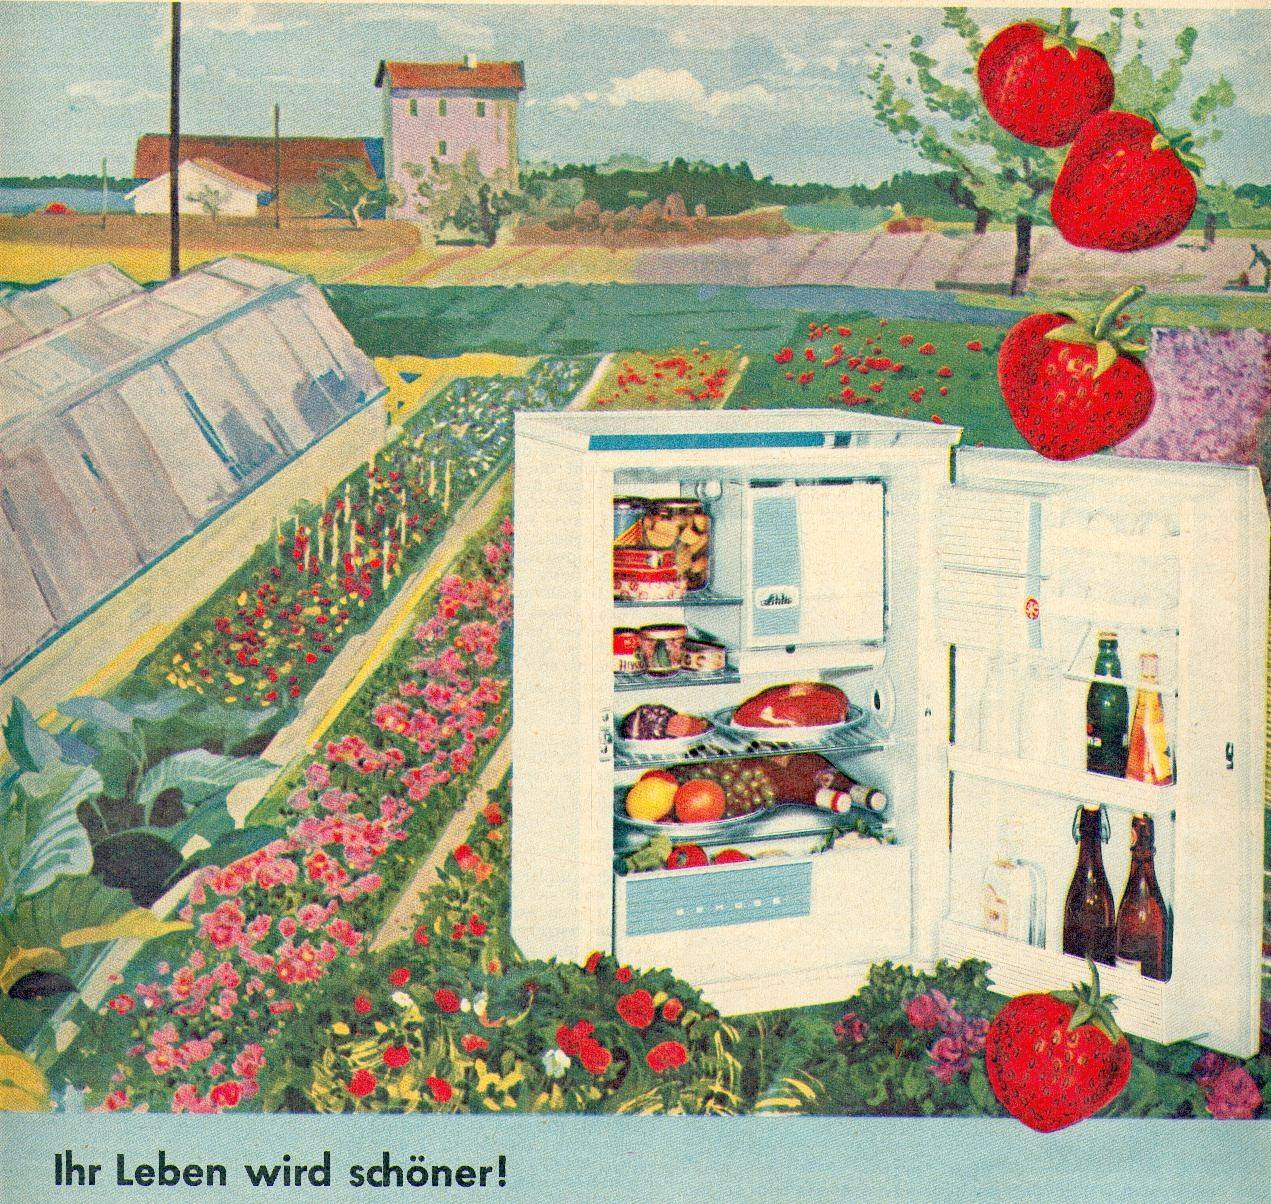
\includegraphics[width=0.73\textwidth]{./History/Spiekermann1.jpg}
    
    \caption{\itshape Cultivation and Civilization: Advertisement of Linde refrigerator, 1959}%\label{fig:profxxx}
   \end{center}
\end{figure}

\begin{}
  \begin{center}
    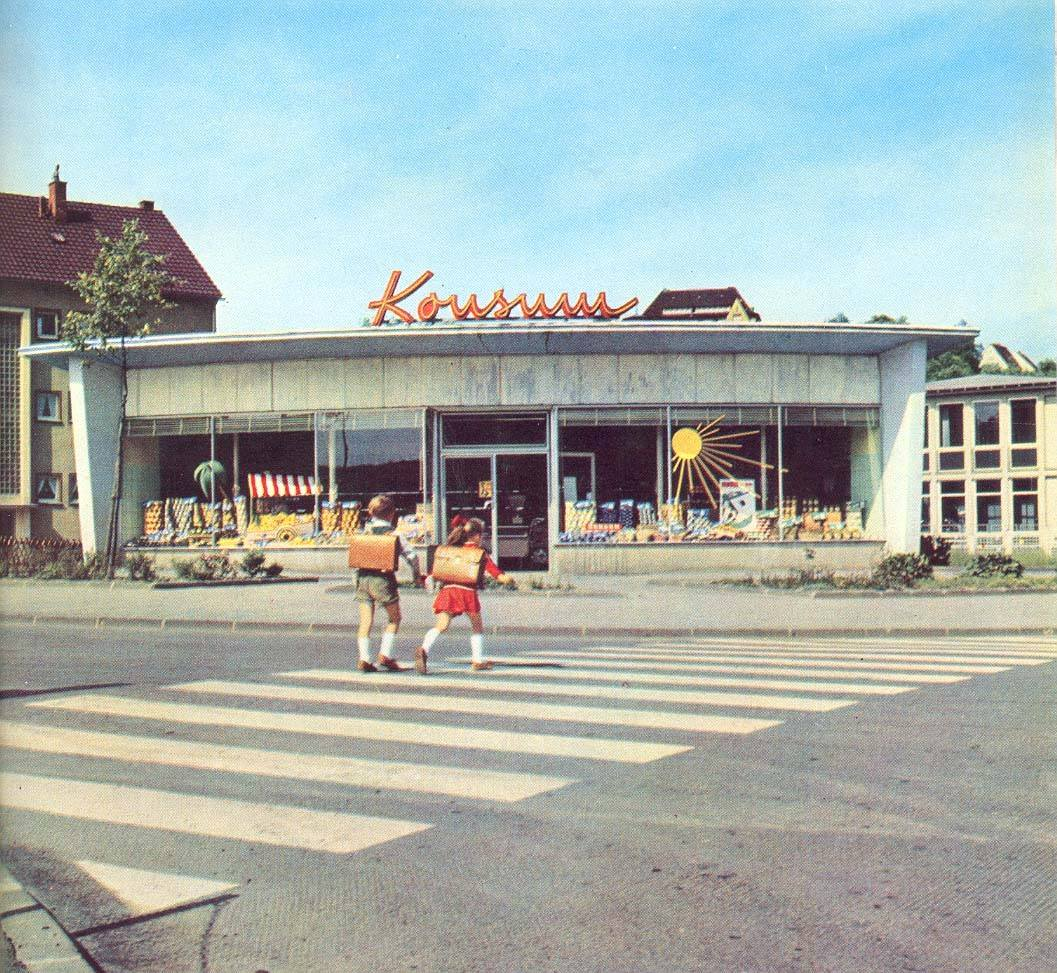
\includegraphics[width=0.72\textwidth]{./History/Spiekermann2.jpg}
    
    \caption{\itshape On the way to a unknown world of affluence, Dortmund 1959}%\label{fig:profxxx}
   \end{center}
\end{figure}

\vspace{0.3cm}
In addition to this project Uwe Spiekermann continued work in his main research areas, mainly in the fields of marketing and retailing. Additionally he arranged (together with two colleagues) a conference on the \textit{History of beer consumption and marketing in $19^{\rm th}$ and $20^{\rm th}$ century}, sponsored by the Gesellschaft f\"{u}r Westf\"{a}lische Wirtschaftsgeschichte, which will take place in Dortmund in June 2007.

\vspace{0.6cm}


\textbf{Funded Projects}\\[-0.25cm]
\begin{enumerate}
\item[$\bullet$]   Scholarship of the Deutsche Forschungsgemeinschaft for the Project \textit{K\"{u}nstliche Kost. Die Durchsetzung der Wissensgesellschaft und die Erfindung der modernen Ern�hrung in Deutschland 1880-2000} (01/2006; 06/2006ff.)
\end{enumerate}



\vspace{0.6cm}
\textbf{Other Professional Activities}\\[-0.25cm]
\begin{enumerate}
\item[$\bullet$] Editorial Committee of "Food and Foodways" (Taylor \& Francis)
\item[$\bullet$] Steering group of the "New Nutrition Science Project" (Global network, supported by the International Union of Nutritionists)
\item[$\bullet$] Scientific advisory board of "Ern\"{a}hrung im Fokus" (Aid)
\item[$\bullet$] Scientific advisory board of "OSSENA - Ern\"{a}hrungsqualit\"{a}t als Lebensqualit\"{a}t" (Research project, financed by the Federal Ministry of Education and Research)
\item[$\bullet$] Scientific Jury of the "F\"{o}rderpreis Ern\"{a}hrungskultur", sponsored by the Johannes Fehr GmbH \& Co. KG
\item[$\bullet$] Visiting lecturer at the University of Vienna, Department of Nutritional Sciences: Lecture/Seminar "Kulturgeschichte der Ern\"{a}hrung"
\item[$\bullet$] Several Radio-Interviews with NDR, WDR, SWR, MDR, mainly on the history of nutrition and retailing.
\end{enumerate}
\newpage
%Publications for History

%the function for the book publication could be as follows [it was not implemented here]
%1=author;2=year;3=title;4=publisher + comments
%\newcommand{\book}[4]{#1 (#2). \textit{#3}. #4}

\newpage

\subsection{Publications}




	\paragraph{Books} \textit{ }
	
\bigskip	


Dooley, B. (Ed.) (2006). \textit{Energy and culture: Perspectives on the power to work}. Burlington, VT: Ashgate. \\ 

Fischer-Tin\'{e}, H. (2006). \textit{Ausnahmezustand}. Novel by Nirmal Verma, translated from Hindi by H. Fischer-Tin\'{e}, \& H. Bauhaus-L\"{o}tzke. Heidelberg: Draupadi.\\ 

Frey, M. (2006). \textit{Dekolonisierung in S\"{u}dostasien. Die Vereinigten Staaten und die Aufl\"{o}sung der europ\"{a}ischen Kolonialreiche}. M\"{u}nchen: Oldenbourg.\\ 

Leutner, M., Spakowski, N., \& Yu, C.M. (Eds.) (2006). \textit{Gonghe shidai de Zhongguo fun\"{u} (Women in China. The Republican Period in Historical Perspective)}. Taipei: Rive Gauche Publishing, in press.\\ 

Paulmann, J. (2006). \textit{Die Haltung der Zur\"{u}ckhaltung: Ausw\"{a}rtige Selbstdarstellungen nach 1945 und die Suche nach einem erneuerten Selbst-verst\"{a}ndnis in der Bundesrepublik} (= Schriftenreihe der Wilhelm und Helene Kaisen-Stiftung), Bremen: Kaisen-Stiftung.\\ 

Spakowski, N., \& Milwertz, C. (Eds.) (2006). \textit{Women and gender in Chinese Studies. Special issue of Chinese History and Society/Berliner China-Hefte}, 29.\\ 



\paragraph{Articles \& Chapters}\textit{ }

\bigskip


Dooley, B. (2006). Art and information brokerage in the career of Don Giovanni de' Medici. In H. Cools, M. Keblusek, \& B. Noldus (Eds.), \textit{Your Humble Servant} (pp. 81-96). Hilversum: Verloren.\\ 

Fischer-Tin\'{e}, H. (2006). Global civil society and the forces of empire. The Salvation Army, British imperialism and the "pre-history" of NGOs. In S. Conrad, \& D. Sachsenmaier (Eds.), \textit{Conceptions of world order: Global historical approaches} (pp. 25-57). New York: Palgrave, in press.\\ 

Fischer-Tin\'{e}, H. (2006). Stadt der Pal\"{a}ste? - Europ\"{a}ische Lebenswelten im kolonialen Kalkutta. In R. Ahuja, \& C. Brosius (Eds.), \textit{Megast\"{a}dte in Indien: Mumbai, Delhi, Calcutta} (pp. 241-256). Heidelberg: Draupadi. \\ 

Fischer-Tin\'{e}, H. (2006). "Deep Occidentalism"? - Europa und der Westen in der Wahrnehmung hinduistischer Intellektueller und Reformer (ca. 1890-1930). \textit{Journal of Modern European History, 4}(2), 171-203.\\ 

Fischer-Tin\'{e}, H. (2006). From \textit{Brahmacharya} to conscious race culture: Indian nationalism, Hindu tradition and Victorian discourses of science. In C. Bates (Ed.), \textit{Beyond representation. The construction of identity in colonial India }(pp. 230-59). New Delhi: Oxford University Press.\\ 

Fischer-Tin\'{e}, H. (2006). Ananda Marga. In C. Auffahrt, H.-G. Kippenberg, \& A. Michaels (Eds.), \textit{W\"{o}rterbuch der Religionen }(p. 32). Stuttgart: Kr\"{o}ner.\\ 

Fischer-Tin\'{e}, H. (2006). Arya Samaj. In C. Auffahrt, H.-G. Kippenberg, \& A. Michaels (Eds.), \textit{W\"{o}rterbuch der Religionen }(p. 45). Stuttgart: Kr\"{o}ner.\\ 

Fischer-Tin\'{e}, H. (2006). Brahmo Samaj. In C. Auffahrt, H.-G. Kippenberg, \& A. Michaels (Eds.), \textit{W\"{o}rterbuch der Religionen }(p. 80). Stuttgart: Kr\"{o}ner.\\ 

Fischer-Tin\'{e}, H. (2006). Dayanand Sarasvati. In C. Auffahrt, H.-G. Kippenberg, \& A. Michaels (Eds.), \textit{W\"{o}rterbuch der Religionen }(p. 103). Stuttgart: Kr\"{o}ner.\\ 

Fischer-Tin\'{e}, H. (2006). Keshab Chandra Sen. In C. Auffahrt, H.-G. Kippenberg, \& A. Michaels (Eds.), \textit{W\"{o}rterbuch der Religionen} (p. 280). Stuttgart: Kr\"{o}ner.\\ 

Fischer-Tin\'{e}, H. (2006). Krishnamurti. In C. Auffahrt, H.-G. Kippenberg, \& A. Michaels (Eds.), \textit{W\"{o}rterbuch der Religionen} (p. 296). Stuttgart: Kr\"{o}ner.\\ 

Fischer-Tin\'{e}, H. (2006). Maharishi Mahesh Yogi. In C. Auffahrt, H.-G. Kippenberg, \& A. Michaels (Eds.), \textit{W\"{o}rterbuch der Religionen} (p. 318). Stuttgart: Kr\"{o}ner.\\ 

Fischer-Tin\'{e}, H. (2006). Neohinduismus. In C. Auffahrt, H.-G. Kippenberg, \& A. Michaels (Eds.), \textit{W\"{o}rterbuch der Religionen} (pp. 370-371). Stuttgart: Kr\"{o}ner.\\ 

Fischer-Tin\'{e}, H. (2006). Radhakrishnan. In C. Auffahrt, H.-G. Kippenberg, \& A. Michaels (Eds.), \textit{W\"{o}rterbuch der Religionen} (p. 419). Stuttgart: Kr\"{o}ner.\\ 

Fischer-Tin\'{e}, H. (2006). Rajneesh. In C. Auffahrt, H.-G. Kippenberg, \& A. Michaels (Eds.), \textit{W\"{o}rterbuch der Religionen} (p. 419). Stuttgart: Kr\"{o}ner.\\ 

Fischer-Tin\'{e}, H. (2006). Ramana Maharshi. In C. Auffahrt, H.-G. Kippenberg, \& A. Michaels (Eds.), \textit{W\"{o}rterbuch der Religionen} (p. 420). Stuttgart: Kr\"{o}ner.\\ 

Fischer-Tin\'{e}, H. (2006). Sri Aurobindo. In C. Auffahrt, H.-G. Kippenberg, \& A. Michaels (Eds.), \textit{W\"{o}rterbuch der Religionen} (p. 496). Stuttgart: Kr\"{o}ner.\\ 

Fischer-Tin\'{e}, H. (2006). Sundar Singh. In C. Auffahrt, H.-G. Kippenberg, \& A. Michaels (Eds.), \textit{W\"{o}rterbuch der Religionen} (p. 504). Stuttgart: Kr\"{o}ner.\\ 

Fischer-Tin\'{e}, H. (2006). Tagore (Debendranath). In C. Auffahrt, H.-G. Kippenberg, \& A. Michaels (Eds.), \textit{W\"{o}rterbuch der Religionen} (p. 509). Stuttgart: Kr\"{o}ner.\\ 

Fischer-Tin\'{e}, H. (2006). Tagore (Rabindranath). In C. Auffahrt, H.-G. Kippenberg, \& A. Michaels (Eds.), \textit{W\"{o}rterbuch der Religionen} (p. 509). Stuttgart: Kr\"{o}ner.\\ 

Fischer-Tin\'{e}, H. (2006). Vivekananda. In C. Auffahrt, H.-G. Kippenberg, \& A. Michaels (Eds.), \textit{W\"{o}rterbuch der Religionen} (p. 558). Stuttgart: Kr\"{o}ner.\\ 

Frey, M. (2006). Die Vereinigten Staaten und die Dritte Welt w\"{a}hrend des Kalten Krieges. In B. Greiner, \& D. Walther (Eds.), \textit{Hei�e Kriege im Kalten Krieg} (pp. 27-56). Hamburg: Hamburger Edition. \\ 

Frey, M. (2006). Zivilgesellschaft in historischer Perspektive: Die Niederlande und Deutschland im 19. Jahrhundert. \textit{Zentrum f\"{u}r Niederlande-Studien Jahrbuch f\"{u}r 2005, 16}, 11-32.\\ 

Frey, M. (2006). Mao Zedong. Nationalist und Despot. In S. F\"{o}rster, \& M. P\"{o}hlmann (Eds.), \textit{Kriegsherren der Weltgeschichte. 22 Historische Portraits} (pp. 357-372). M\"{u}nchen: C.H. Beck.\\ 

Spakowski, N., \& Milwertz, C. (2006). Introduction: Women and gender in Chinese Studies and the Women and Gender in Chinese Studies Network (WAGNet). In N. Spakowski, \& C. Milwertz (Eds.), \textit{Women and Gender in Chinese Studies}. Special issue of \textit{Chinese History and Society/Berliner China-Hefte, 29}, 3-4.\\ 

Spiekermann, U. (2006). From neighbour to consumer. The transformation of retailer-consumer relationships in twentieth-century Germany. In F. Trentmann (Ed.), \textit{The making of the consumer. Knowledge, power and identity in the modern world} (pp. 147-174). Oxford: Berg.\\ 

Spiekermann, U. (2006). Warum scheitert Ern\"{a}hrungskommunikation? In Aid e.V. (Ed.), \textit{Ern\"{a}hrungskommunikation. Neue Wege - neue Chancen?}. (pp. 11-20). Bonn: Aid.\\ 

Spiekermann, U. (2006). Warum scheitert die Ern\"{a}hrungskommunikation? Eine Antwort aus kulturwissenschaftlicher Perspektive. In E. Barl\"{o}sius, \& R. Rehaag (Ed.), \textit{Anforderungen an eine \"{o}ffentliche Ern\"{a}hrungskommunikation} (pp. 39-51). Berlin: Wissenschaftszentrum.\\ 

Spiekermann, U. (2006). Warenwelten. Die Normierung der Nahrungsmittel in Deutschland 1880-1930. In R.-E. Mohrmann (Ed.), \textit{Essen und Trinken in der Moderne} (pp. 99-124). M\"{u}nster: Waxmann.\\ 

Spiekermann, U. (2006). Brown bread for victory: German and British wholemeal politics in the interwar period. In F. Trentmann, \& F. Just (Ed.), \textit{Food and conflict in Europe in the age of the two World Wars} (pp. 143-171). Basingstoke: Palgrave Macmillan.\\ 

\newpage
%Lecture Talks for Psychology

\newpage  
\subsection{Invited Scientific Lectures and Talks}

{\hyphenpenalty=5000
\begin{flushleft}
January 2006\\[0.5cm]
\end{flushleft}
\begin{tabular}{lp{13.4cm}}
 Speaker:	&   Jens F\"{o}rster \\
 Place: 	 & Palm Springs, CA, USA\\
 Event:   &	Meeting of the Society for Personality and Social Psychology (SPSP) \\
 Title: &	Catharsis Revisited: Inhibition of Aggression-Related Constructs after Goal-Fulfillment (with Markus Denzler and Nira Liberman) \\ \\
\end{tabular}
\begin{tabular}{lp{13.4cm}}
 Speaker:	&   Jens F\"{o}rster \\
 Place: 	 & Palm Springs, CA, USA\\
 Event:   &	Meeting of the Society for Personality and Social Psychology (SPSP) \\
 Title: &	Abstract and Concrete Thinking: The Effects of Motivational Cues on Thinking Styles (with Stefanie Kuschel) \\ \\
\end{tabular}
\begin{tabular}{lp{13.4cm}}
 Speaker:	&   Jens F\"{o}rster \\
 Place: 	 & Palm Springs, CA, USA\\
 Event:   &	7th Annual Meeting of the Society for Personality and Social Psychology (SPSP)\\
 Title: &	Regulatory Focus and the Evaluation of Visual Arts - Implications for Motivational Effects on Attitudes (with Katrin Schimmel)\\ \\
\end{tabular}
\begin{tabular}{lp{13.4cm}}
 Speaker:	&   Jens F\"{o}rster \\
 Place: 	 & Palm Springs, CA, USA\\
 Event:   &	7th Annual Meeting of the Society for Personality and Social Psychology (SPSP)\\
 Title: &	Novelty Theory\\ \\
\end{tabular}
\begin{tabular}{lp{13.4cm}}
 Speaker:	&   Jens F\"{o}rster \\
 Place: 	 & Columbia University, New York, NY, USA\\
 Event:   &	Guest lecture\\
 Title: &	Novelty Theory\\ \\
\end{tabular}
\begin{tabular}{lp{13.4cm}}
 Speaker:	&   Jens F\"{o}rster \\
 Place: 	 & Bremen\\
 Event:   &	Conference "Jazzahead"\\
 Title: &	Zwischen Chaos und Sicherheit: Jazz als Modell einer balancierten Organisation mit innovativem Charakter\\ \\
\end{tabular}
\begin{tabular}{lp{13.4cm}}
 Speaker:	&   Jens F\"{o}rster \\
 Place: 	 &Zentrum f\"{u}r feministische Studien, Universit\"{a}t Bremen\\
 Event:   &	Guest lecture\\
 Title: &	Zur Sozialpsychologie der Vorurteile\\ \\
\end{tabular}
\begin{tabular}{lp{13.4cm}}
 Speaker:	&  	Ulrich K\"{u}hnen \\
 Place: 	 &Palm Springs, CA, USA\\
 Event:   &	7th Annual Meeting of the Society for Personality and Social Psychology (SPSP)\\
 Title: &	Consequences of Self-Regulatory Foci: Prevention Leads to Analytic Processing for Independents, but to Holistic Processing for Interdependents\\ \\
\end{tabular}
	

\newpage
\begin{flushleft}
February 2006\\[0.5cm]
\end{flushleft}
\begin{tabular}{lp{13.4cm}}
 Speaker:	&  Adele Diederich \\
 Place: 	 &Albert-Ludwigs-Universit\"{a}t Freiburg\\
 Event:   &	Freiburg Workshop of Diffusion Models\\
 Title: &		Diffusion Models for Multiattribute Choice Alternatives\\ \\
\end{tabular}
\begin{tabular}{lp{13.4cm}}
 Speaker:	&  Jens F\"{o}rster \\
 Place: 	 &M\"{u}nchen\\
 Event:   &	Forum 2006 der Trurnit Gruppe\\
 Title: &		Motivierte Mitarbeiter. Sozialpsychologische Erkenntnisse und Anwendungen\\ \\
\end{tabular}
	


\begin{flushleft}
March 2006\\[0.5cm]
\end{flushleft}
\begin{tabular}{lp{13.4cm}}
 Speaker:	&  Daniela Bockhorst \\
 Place: 	 &Mainz\\
 Event:   &	Tagung experimentell arbeitender Psychologen, TeaP\\
 Title: &		Personelle und situative Moderatoren riskanter Entscheidungen\\ \\
\end{tabular}
\begin{tabular}{lp{13.4cm}}
 Speaker:	&  Adele Diederich \\
 Place: 	 &T\"{u}bingen\\
 Event:   &	9. T\"{u}binger Wahrnehmungskonferenz\\
 Title: &		Why Two "Distracters" Are Better Than One: Modelling the Effect of Non-Target Auditory and Tactile Stimuli on Visual Saccadic Reaction Time\\ \\
\end{tabular}
\begin{tabular}{lp{13.4cm}}
 Speaker:	&  Adele Diederich \\
 Place: 	 &T\"{u}bingen\\
 Event:   &	9. T\"{u}binger Wahrnehmungskonferenz\\
 Title: &		Separating Multisensory Integration from Unspecific Warning Effects in Saccadic Reaction Time\\ \\
\end{tabular}
\begin{tabular}{lp{13.4cm}}
 Speaker:	&  Jens F\"{o}rster \\
 Place: 	 &Mainz\\
 Event:   &	Tagung experimentell arbeitender Psychologen, TeaP\\
 Title: &		Globale und lokale Wahrnehmung beeinflusst Assimilation und Kontrast bei sozialen Urteilen (with Stefanie Kuschel)\\ \\
\end{tabular}
\begin{tabular}{lp{13.4cm}}
 Speaker:	&  Jens F\"{o}rster \\
 Place: 	 &Mainz\\
 Event:   &	Tagung experimentell arbeitender Psychologen, TeaP\\
 Title: &		Fit macht Jungs attraktiv: Einfluss von regulatorischem Fit auf Personenbeurteilung (with Laura Dannenberg)\\ \\
\end{tabular}
\begin{tabular}{lp{13.4cm}}
 Speaker:	&  Jens F\"{o}rster \\
 Place: 	 &Mainz\\
 Event:   &	Tagung experimentell arbeitender Psychologen, TeaP\\
 Title: &		Odi et amo - Ich hasse und ich liebe. Der Einfluss von aggressiver und friedfertiger Zielerf\"{u}llung auf die Verf\"{u}gbarkeit von Aggression und auf aggressives Verhalten (with Markus Denzler and Nira Liberman)\\ \\
\end{tabular}
\begin{tabular}{lp{13.4cm}}
 Speaker:	&  Jens F\"{o}rster \\
 Place: 	 &Mainz\\
 Event:   &	Tagung experimentell arbeitender Psychologen, TeaP\\
 Title: &		Ann\"{a}herung und Vermeidung: Wie motivationale Faktoren Denkstile und die Enkodierung von Bedeutung und Details beeinflussen (with Stefanie Kuschel)\\ \\
\end{tabular}
\begin{tabular}{lp{13.4cm}}
 Speaker:	&  Rike Steenken \\
 Place: 	 &Oldenburg\\
 Event:   &	International Graduate School for Neurosensory Science and Systems\\
 Title: &		Multisensory Interaction: Unconscious Spatial Priming in an Audio-Visual Paradigm?\\ \\
\end{tabular}



\begin{flushleft}
April 2006\\[0.5cm]
\end{flushleft}
\begin{tabular}{lp{13.4cm}}
 Speaker:	&  Jens F\"{o}rster \\
 Place: 	 &Glocke, Bremen\\
 Event:   &	Sichtweisen in der Glocke\\
 Title: &		Tempo \& Termine - Wie die Zeit unser Leben bestimmt (with Bernhard Kramer)\\ \\
\end{tabular}
\begin{tabular}{lp{13.4cm}}
 Speaker:	&  Jens F\"{o}rster \\
 Place: 	 &Universit\"{a}t Dresden\\
 Event:   &	Universit\"{a}ts-Kolloquium\\
 Title: &		Die Psychologie der Gedankenunterdr\"{u}ckung\\ \\
\end{tabular}



\begin{flushleft}
May 2006\\[0.5cm]
\end{flushleft}
\begin{tabular}{lp{13.4cm}}
 Speaker:	&  Adele Diederich \\
 Place: 	 &Universit\"{a}t Osnabr\"{u}ck\\
 Event:   &	Workshop on Neuroscience and Neuroeconomics, FB Wirtschaftswissenschaften\\
 Title: &		Dynamic-Stochastic Models of Decision Making\\ \\
\end{tabular}
\begin{tabular}{lp{13.4cm}}
 Speaker:	&  Jens F\"{o}rster \\
 Place: 	 &Jena\\
 Event:   &	Socdoc meeting\\
 Title: &		Keynote Talk: Seven Principles of Self Regulation\\ \\
\end{tabular}
\begin{tabular}{lp{13.4cm}}
 Speaker:	&	Jens F\"{o}rster \\
 Place: 	 &Universiteit van Amsterdam, Netherlands\\
 Event:   &	Colloquium\\
 Title: &		New Perspectives on Social Psychology\\ \\
\end{tabular}
\begin{tabular}{lp{13.4cm}}
 Speaker:	&	Arvid Kappas \\
 Place: 	 &  Universit\�{e} Louvain-La-Neuve, Belgium \\
 Event:   &	2nd Meeting of the Consortium of European Research on Emotion (CERE)\\
 Title: &		Appraisal and Emotion Regulation (Keynote Address)\\ \\
\end{tabular}
\begin{tabular}{lp{13.4cm}}
 Speaker:	&	Arvid Kappas \\
 Place: 	 & Universit\�{e} Louvain-La-Neuve, Belgium\\
 Event:   &	2nd Meeting of the Consortium of European Research on Emotion (CERE)\\
 Title: &		Implicit Associations between the Concepts of Friends/Strangers with Showing/Hiding Emotions: An Indirect Investigation on the Relationship between Emotions and Expressions (with Dennis K\"{u}ster)\\ \\
\end{tabular}




\begin{flushleft}
June 2006\\[0.5cm]
\end{flushleft}
\begin{tabular}{lp{13.4cm}}
 Speaker:	&  Adele Diederich \\
 Place: 	 &Dublin, Ireland\\
 Event:   &	7th Annual Meeting of the International Multisensory Research Forum\\
 Title: &		Separating Multisensory Integration from Unspecific Warning Effects in Saccadic Reaction Time\\ \\
\end{tabular}
\begin{tabular}{lp{13.4cm}}
 Speaker:	&  Adele Diederich \\
 Place: 	 &Dublin, Ireland\\
 Event:   &	7th Annual Meeting of the International Multisensory Research Forum\\
 Title: &		Audio-Visual Integration of Letters and Speech: From Unimodal to Bimodal Subjective Representation\\ \\
\end{tabular}
\begin{tabular}{lp{13.4cm}}
 Speaker:	&  Adele Diederich \\
 Place: 	 &Dublin, Ireland\\
 Event:   &	7th Annual Meeting of the International Multisensory Research Forum\\
 Title: &		Visual-Tactile Integration: Does Stimulus Duration Influence the Relative Amount of Response Enhancement? (with Stefan Rach)\\ \\
\end{tabular}



\begin{flushleft}
July 2006\\[0.5cm] 
\end{flushleft}
\begin{tabular}{lp{13.4cm}}
 Speaker:	& Jens F\"{o}rster \\
 Place: 	 &M\"{u}nchen\\
 Event:   &	Tagung der Jungen Akademie\\
 Title: &		Keynote Talk: Wo bleibt die Zeit?\\ \\
\end{tabular}
\begin{tabular}{lp{13.4cm}}
 Speaker:	&  Jens F\"{o}rster \\
 Place: 	 &Kurt Lewin Institute, Groningen, Netherlands\\
 Event:   &	Kurt Lewin Workshop\\
 Title: &		KeynoteTalk: Seven Principles of Self Regulation\\ \\
\end{tabular}
\begin{tabular}{lp{13.4cm}}
 Speaker:	&  Jens F\"{o}rster \\
 Place: 	 &MPI Leipzig\\
 Event:   &	Colloquium\\
 Title: &		Solving Problems in a Social Context: The Motivational Underpinnings of Creative and Analytic Thinking\\ \\
\end{tabular}
\begin{tabular}{lp{13.4cm}}
 Speaker:	&  Arvid Kappas \\
 Place: 	 &University of Reading, England\\
 Event:   &	Psypag Annual Conference\\
 Title: &		Correlates of Hope: A Psychophysiological Perspective (with Malathy Rengamani and Sue Weaver)\\ \\
\end{tabular}
\begin{tabular}{lp{13.4cm}}
 Speaker:	&  Ulrich K\"{u}hnen \\
 Place: 	 &Universit\"{a}t Heidelberg\\
 Event:   &	Concluding Event of the "Experimentalpsychologisches Praktikum"\\
 Title: &	Kultur, Kontext und Kultur\\ \\
\end{tabular}
\begin{tabular}{lp{13.4cm}}
 Speaker:	&  Bettina Olk \\
 Place: 	 &Zurich, Switzerland\\
 Event:   &	Joint Meeting of the International Neuropsycholgical Society, Swiss Society of Neuropsychology, German Society of Neuropsychology\\
 Title: &	Volitional Orienting in Patients with Right-Hemisphere Lesions\\ \\
\end{tabular}
\begin{tabular}{lp{13.4cm}}
 Speaker:	&  Bettina Olk \\
 Place: 	 &M\"{u}nchen\\
 Event:   &	Colloquium of the Department of General Psychology, Ludwig-Maximilians-Universit\"{a}t M\"{u}nchen\\
 Title: &	Integration of Reflexive and Volitional Orienting\\ \\
\end{tabular}



\begin{flushleft}
August 2006\\[0.5cm] 
\end{flushleft}
\begin{tabular}{lp{13.4cm}}
 Speaker:	&  Adele Diederich \\
 Place: 	 &Vancouver, Canada\\
 Event:   &	39th Annual Society of Mathematical Psychology Meeting\\
 Title: &		Audiovisual Integration of Letters and Speech: A Fechnerian Scaling Analysis\\ \\
\end{tabular}
\begin{tabular}{lp{13.4cm}}
 Speaker:	&  Adele Diederich \\
 Place: 	 &Vancouver, Canada\\
 Event:   &	39th Annual Society of Mathematical Psychology Meeting\\
 Title: &		Modeling the Effects of Payoffs on Response Bias in a Perceptual Discrimination Task\\ \\
\end{tabular}
\begin{tabular}{lp{13.4cm}}
 Speaker:	&  Adele Diederich \\
 Place: 	 &University of Surrey, Guildford, England\\
 Event:   &	Workshop on Biologically Inspired Information Fusion\\
 Title: &		Distance From Discriminability: A Fechnerian Scaling Approach to Multisensory Integration\\ \\
\end{tabular}
\begin{tabular}{lp{13.4cm}}
 Speaker:	&  Arvid Kappas \\
 Place: 	 &Dartmouth College, New Hampshire, USA\\
 Event:   &	Minary Conference in Honor of Robert E. Kleck\\
 Title: &		People in Interaction: In their Muscles and their Brains!\\ \\
\end{tabular}





\begin{flushleft}
September 2006\\[0.5cm]
\end{flushleft}
\begin{tabular}{lp{13.4cm}}
 Speaker:	&  Adele Diederich \\
 Place: 	 &Brest, France\\
 Event:   &	37th European Mathematical Psychology Group meeting\\
 Title: &		A Fechnerian Analysis of Visual-Auditory Integration\\ \\
\end{tabular}
\begin{tabular}{lp{13.4cm}}
 Speaker:	&  Jens F\"{o}rster \\
 Place: 	 &N\"{u}rnberg\\
 Event:   &	45th Congress of the Deutsche Gesellschaft f\"{u}r Psychologie (DGPs)\\
 Title: &		Odi et amo - Ich hasse und ich liebe. Der Einfluss von aggressiver und friedfertiger Zielerf\"{u}llung auf die Verf\"{u}gbarkeit von Aggression und auf aggressives Verhalten (with Markus Denzler and Nira Liberman)\\ \\
\end{tabular}
\begin{tabular}{lp{13.4cm}}
 Speaker:	&  Jens F\"{o}rster \\
 Place: 	 &N\"{u}rnberg\\
 Event:   &	45th Congress of the Deutsche Gesellschaft f\"{u}r Psychologie (DGPs)\\
 Title: &		Selbstregulation und Denkstile: Einfluss motivationaler Orientierungen auf die Enkodierung von Bedeutung und Details (with Stefanie Kuschel)\\ \\
\end{tabular}
\begin{tabular}{lp{13.4cm}}
 Speaker:	&  Jens F\"{o}rster \\
 Place: 	 &N\"{u}rnberg\\
 Event:   &	45th Congress of the Deutsche Gesellschaft f\"{u}r Psychologie (DGPs)\\
 Title: &		Der Einfluss regulatorischer Foki auf Einstellungen zu Kunst (with Katrin Schimmel)\\ \\
\end{tabular}
\begin{tabular}{lp{13.4cm}}
 Speaker:	&  Jens F\"{o}rster \\
 Place: 	 &N\"{u}rnberg\\
 Event:   &	45th Congress of the Deutsche Gesellschaft f\"{u}r Psychologie (DGPs)\\
 Title: &		Ann\"{a}herungs- und Vermeidungsmotivation beeinflusst Assimilation und Kontrast bei sozialen Urteilen (with R. Friedman)\\ \\
\end{tabular}
\begin{tabular}{lp{13.4cm}}
 Speaker:	&  Jens F\"{o}rster \\
 Place: 	 &Heidelberg\\
 Event:   &	Milieus of Creativity\\
 Title: &		Creativity in Context: the Social Psychology of Creativity\\ \\
\end{tabular}
\begin{tabular}{lp{13.4cm}}
 Speaker:	&  Jens F\"{o}rster \\
 Place: 	 &Pultusk, Poland\\
 Event:   &	8th European Social Cognition Network: Transfer of Knowledge Conference\\
 Title: &		Cathartic Effects Revisited. The Impact of Goals on Aggressive Thoughts and Aggressive Behavior (with Markus Denzler and Nira Liberman)\\ \\
\end{tabular}
\begin{tabular}{lp{13.4cm}}
 Speaker:	&  Arvid Kappas \\
 Place: 	 &Coventry University, England\\
 Event:   &	34th Annual Scientific Meeting of the British Association for Cognitive Neuroscience (formerly British Psychophysiology Society)\\
 Title: &		Individual Differences in Dispositional Hope in Relation to Cardiovascular Reactivity, Pain Perception and Stress Appraisals (with Malathy Rengamani and Sue Weaver)\\ \\
\end{tabular}
\begin{tabular}{lp{13.4cm}}
 Speaker:	&  Ulrich K\"{u}hnen \\
 Place: 	 &N\"{u}rnberg\\
 Event:   &	45th Congress of the Deutsche Gesellschaft f\"{u}r Psychologie (DGPs)\\
 Title: &		Selbstkonzept und freier Wille: Sind "wir" weniger frei als "ich?" (with Laura Dannenberg)\\ \\
\end{tabular}



\newpage
\begin{flushleft}
October 2006\\[0.5cm] 
\end{flushleft}
\begin{tabular}{lp{13.4cm}}
 Speaker:	&  Jens F\"{o}rster \\
 Place: 	 &Philadelphia, USA\\
 Event:   &	2006 Conference of the Society of Experimental Social Psychology (SESP)\\
 Title: &		Seven Principles of Self Regulation\\ \\
\end{tabular}
\begin{tabular}{lp{13.4cm}}
 Speaker:	&  Jens F\"{o}rster \\
 Place: 	 &Chicago, USA\\
 Event:   &	Colloquium Chicago Business School\\
 Title: &	Novelty Theory: Implications for Abstract and Concrete Processing Styles\\ \\
\end{tabular}
\begin{tabular}{lp{13.4cm}}
 Speaker:	&  Arvid Kappas \\
 Place: 	 &Vancouver, BC, Canada\\
 Event:   &	46th Annual Meeting of the Society for Psychophysiological Research\\
 Title: &		Priming "We" or "They" Affects Level of Orbicularis Oculi Activity in Response to Funny Films: An Investigation on the Relationship between Emotions and Facial Activity (with Dennis K\"{u}ster)\\ \\
\end{tabular}
\begin{tabular}{lp{13.4cm}}
 Speaker:	& Bettina Olk \\
 Place: 	 &Vancouver General Hospital Eye Care Center, Canada\\
 Event:   &	Invited talk\\
 Title: &	Mechanisms of Reflexive and Volitional Orienting\\ \\
\end{tabular}


\begin{flushleft}
November 2006\\[0.5cm]
\end{flushleft}
\begin{tabular}{lp{13.4cm}}
 Speaker:	&  Adele Diederich \\
 Place: 	 &Houston, TX, USA\\
 Event:   &	47th Annual Meeting of the Psychonomic Society\\
 Title: &		Audiovisual Integration of Letters and Speech: A Fechnerian Scaling Analysis\\ 
\end{tabular}
\begin{tabular}{lp{13.4cm}}
 Speaker:	&  Adele Diederich \\
 Place: 	 &Magdeburg\\
 Event:   &	SFB-Jahrestagung of Sonderforschungsbereich/TransRegio 31 "Das aktive Geh\"{o}r"\\
 Title: &		An Experiment on Audio-Visual Integration of Letters (with Stefan Rach)\\ \\
\end{tabular}
\begin{tabular}{lp{13.4cm}}
 Speaker:	&  Amina \"{O}zelsel \\
 Place: 	 &Glocke, Bremen\\
 Event:   &	Sichtweisen\\
 Title: &		S\"{u}�es Ja und bitteres Nein (with Franziska Deutsch)\\ \\
\end{tabular}
\begin{tabular}{lp{13.4cm}}
 Speaker:	&  Bettina Olk \\
 Place: 	 &International University Bremen\\
 Event:   &	Workshop Autismustherapie\\
 Title: &		Aufmerksamkeit und Lernen: Grundlagen\\ \\
\end{tabular}
\begin{tabular}{lp{13.4cm}}
 Speaker:	&  Bettina Olk \\
 Place: 	 &Houston, TX, USA\\
 Event:   &	Psychonomics\\
 Title: &		Rethinking Voluntary and Involuntary Spatial Attention (with Alan Kingstone and Jelena Ristic)\\ \\
\end{tabular}
	



\begin{flushleft}
December 2006\\[0.5cm] 
\end{flushleft}
\begin{tabular}{lp{13.4cm}}
 Speaker:	&  Bettina Olk \\
 Place: 	 &Klinikum Bremen-Ost\\
 Event:   &	6th Conference on Cognitive Neuropsychiatry\\
 Title: &		Eye Movement Patterns as a Sensitive Measure of Deficits in Autism\\ \\
\end{tabular}
\begin{tabular}{lp{13.4cm}}
 Speaker:	&  Rike Steenken \\
 Place: 	 &Oldenburg\\
 Event:   &	International Graduate School for Neurosensory Science and Systems\\
 Title: &	Does Spatial Audio-Visual Interaction Depend on Awareness of Acoustical Stimulus' Locations?\\ \\
\end{tabular}

}

\newpage
\section{Psychology}
\shorttitle{Psychology}
\subsection{Prof. Dr. Adele Diederich}


\textbf{Main Research Interests}\\[-0.25cm]
\begin{enumerate}
\item[$\bullet$]	Perception: Multisensory Interaction
\item[$\bullet$]	Decision Theory: Dynamic Models for Decision Making under Uncertainty
\item[$\bullet$]	Medical Decision Making: Conjoint Analysis (Random Utility Models) in Health Care
\item[$\bullet$]	Psychophysics: Fechnerian Scaling
\item[$\bullet$]	Mathematical Modeling of Cognitive Processes
\end{enumerate}


\vspace{0.6cm}
\textbf{Research Activities}\\[-0.25cm]

Adele Diederich has two main research foci: Perception and Decision-Making. Perceptual processes are typically investigated within one modality only. Triggered by recent physiological findings multisensory research has caught interest of cognitive psychologists as well. Two DFG grants allowed Adele Diederich to continue to study the interaction of different modalities in space and in time with experiments using elementary stimuli and measuring manual response times and saccadic eye movements. Quantitative psychological models were developed for the behavioral results taking into account results from neurophysiological studies of the lower brain structures. During the summer an extensive study with elderly from the Bremen area was conducted. The theory of Fechnerian Scaling makes available a principled way of imposing a metric representing pairwise dissimilarities on any discrete set of stimuli, given the probability with which they are discriminated from each other. Adele Diederich utilizes this approach in testing whether bimodal objects possess emergent features that cannot be predicted from their unimodal (visual and auditory) representations. In the field of decision-making processes Multi-Attribute Decision Field Theory (MDFT) is a theory developed for multiattribute decision problems which take into account both the dynamic and stochastic nature of decision making. Its goal is to describe the motivational and cognitive mechanisms that guide the deliberation process in decisions under uncertainty. Ongoing experiments investigate the influence of payoffs in perception decision tasks. Competing models are included in analyzing the data. Researchers from different fields (Economics, Law, Medicine, Philosophy, and Psychology) initiated a research group on \textit{Priorisierung in der Medizin} (described in Chapter 7 of this research report). Adele Diederich is the coordinator of this research group, meanwhile suggested for funding by evaluators of Deutsche Forschungsgemeinschaft. A book on \textit{Cognitive Modeling} together with J.R. Busemeyer, Indiana University, Bloomington, USA, is in progress. The book is targeted to graduate students in cognitive sciences. It is planned to be finished in 2007.
\vspace{0.6cm}


\textbf{Funded Projects}\\[-0.25cm]
\begin{enumerate}
\item[$\bullet$]   Experimentelle und theoretische Untersuchung r�umlicher und zeitlicher Regeln der multisensorischen Integration, funded by Deutsche Forschungsgemeinschaft
\item[$\bullet$]   Regular minimality principle in relation to decision making and categorization, funded by AFOSR (US Air Force)
\item[$\bullet$]   International Graduate School for Neurosensory Systems and Science funded by Deutsche Forschungsgemeinschaft
\item[$\bullet$]   Sokrates/Erasmus Intensive Program on "Mathematical and Computational Models in the Psychological Sciences (MCMPS)" funded by the European Commission
\end{enumerate}



\vspace{0.6cm}
\textbf{Other Professional Activities}\\[-0.25cm]
\begin{enumerate}
\item[$\bullet$] Editorial Board: Journal of Mathematical Psychology
\item[$\bullet$] Executive Board:  Society of Mathematical Psychology
\item[$\bullet$] Member of the NSF Panel Methodology, Measurement, and Statistics (MMS) 
\item[$\bullet$] Member of the research center Neurosensorik Oldenburg
\item[$\bullet$] Numerous reviews for international journals (e.g., Psychological Review, Journal of Experimental Psychology: General; Psychonomic Bulletin and Review; Journal of Mathematical Psychology; Cognitive Science, etc.) 
\item[$\bullet$] Numerous reviews for funding agencies (DFG, NSF, NWO)
\item[$\bullet$] Coordination (Sprecherin) of the Forschergruppe "Priorisierung in der Medizin"
\item[$\bullet$] Committee work 
	\begin{enumerate}
		\item[-]	Member of the University Promotion Review Committee for the School of Humanities and Social Sciences
		\item[-]	Member of the University Promotion Review Committee for the School of Engineering and Science 
		\item[-]	Member of the  Scientific Computation Committee of CLAMV
		\item[-]	Numerous ad hoc committees
		\item[-]	New Investigator Award of the Society for Mathematical Psychology
	\end{enumerate}
\item[$\bullet$] Mentor in the mentoring program of the Universit\"{a}t Bremen
\item[$\bullet$] Contact person (Vertrauensdozentin) of Friedrich Naumann Stiftung
\item[$\bullet$] Evaluation and selection of fellows for the Studienstiftung des deutschen Volkes
\end{enumerate}





\vspace{0.6cm}
\textbf{PhD-Students}\\[-0.25cm]

Daniela Bockhorst\newline
\textit{Entscheiden unter Unsicherheit: Alters- und geschlechtsspezifische Einfl�sse in alltagsnahen Wahlsituationen}\\[-0.15cm]

Stefan Rach\newline
\textit{A Two-stage Multichannel Diffusion Model of Multisensory Integration}\newline
funded by Deutsche Forschungsgemeinschaft\\[-0.15cm]

Rike Steenken\newline
\textit{Psychophysical Investigation of Unconscious Cross-Modal Priming}\newline
funded by Deutsche Forschungsgemeinschaft

\vspace{0.6cm}
\textbf{Research Personnel}\\[-0.25cm]

Dr. Annette Schomburg\newline 
PostDoc funded by Deutsche Forschungsgemeinschaft
\newpage
\subsection{Prof. Dr. Jens F\"{o}rster}


\textbf{Main Research Interests}\\[-0.25cm]
\begin{enumerate}
\item[$\bullet$]	Social Cognition (Judgment, Perception, Processing Styles, Memory)
\item[$\bullet$]	Self Regulation (Motivation, Self Control, Automatic Goal Pursuit) 
\item[$\bullet$]	Embodiment (Meaning, Expression Patterns, Attitudes, Emotion) 
\item[$\bullet$]	Prejudice (Stereotype Threat, Discrimination, Thought Suppression)
\end{enumerate}


\vspace{0.6cm}
\textbf{Research Activities}\\[-0.25cm]

Jens F\"{o}rster's research focuses on basic principles of information processing and motivation that underlie diverse social phenomena. In 2006, more than 200 experiments have been conducted with the following results: \textit{Global processing styles} (looking at the forest) enhance abstract thinking, creativity, similarity search, abstraction of meaning, and reduce prejudice, whereas {\itshape local processing styles} (looking at the trees) enhance concrete and analytic thinking, dissimilarity search, and detail perception. Global vs. local processing can be elicited by {\itshape approach/avoidance motivation, regulatory focus, positive/negative mood} and {\itshape right/left hemisphere activation}, and studies show that they have similar effects. To illustrate, a study found that if participants compared their athletic skills to high (Michael Schumacher) or low standards (Helmut Kohl), they assimilate their judgments toward the standard when in a good mood (e.g., think that they are more athletic after comparison with Schumacher and less athletic after comparison with Kohl) - whereas contrast effects occurred when in a bad mood (e.g., think they are less athletic after comparison with high and more athletic after comparison with low standards). Three papers were submitted. Further studies examined the impact of {\itshape novelty} on thinking, showing that framing events as novel leads to activation of broader categories than framing events as familiar. A paper is under revision. A cognitive model on {\itshape love} vs. {\itshape sex} was designed. Studies found that unconscious reminders of love make people more creative, enhance face recognition, lead to global processing and Halos, whereas unconscious priming of sex enhances analytic thinking, recognition of verbal information, local processing and reduces Halos. Three papers have been submitted. Moreover, Jens F\"{o}rster finished reviews on unconscious self regulation (one paper is under revision; three book chapters are in press), and two book chapters on embodiment and approach/avoidance motivation were submitted. He is currently editing a book on Social Cognition and a popular book on prejudice has been accepted by dva/Random House and will appear March 2007. 

\vspace{0.6cm}


\textbf{Funded Projects}\\[-0.25cm]
\begin{enumerate}
\item[$\bullet$]   "Perseveranzeffekte bei Kreativit\"{a}t und analytischem Denken", funded by Deutsche Forschungsgemeinschaft 
\item[$\bullet$]   "Motivational Influences on Construct Accessibility", funded by Deutsche Forschungsgemeinschaft
\end{enumerate}



\vspace{0.6cm}
\textbf{Other Professional Activities}\\[-0.25cm]
\begin{enumerate}
\item[$\bullet$] Ad hoc reviewer for the following scientific journals: \textit{Acta Psychologica, Anxiety, Stress, and Coping, Behaviour Research and Therapy, British Journal of Social Psychology, Cognition and Emotion, Cortex, Emotion, European Journal of Social Psychology, Experimental Psychology, Journal of Experimental Psychology: Learning, Memory, \& Cognition, Journal of Experimental Psychology: Human Perception \& Performance, Journal of Experimental Social Psychology, Journal of Personality, Journal of Personality and Social Psychology, Learning and Individual Differences, Personality and Social Psychology Bulletin, Psychological Science, Quarterly Journal of Experimental Psychology, Schweizerische Zeitschrift f�r Psychologie, Self and Identity, Social Cognition, Zeitschrift f�r Psychologie, Zeitschrift f�r Sozialpsychologie, Zeitschrift f�r Experimentelle Psychologie.} 
\item[$\bullet$] Associate editor of \textit{Social Cognition}
\item[$\bullet$] Member of the editorial board of the \textit{European Journal of Social Psychology}
\item[$\bullet$] Member of the editorial board of the \textit{Journal of Personality and Social Psychology}
\item[$\bullet$] Member of the editorial board of \textit{Self and Identity}
\item[$\bullet$] Reviewer for the following organisations: Deutsche Forschungsgemeinschaft (DFG) single projects, ethics guidelines for research, graduate colleges and research groups, Deutsche Gesellschaft f�r Psychologie (Ethics), Deutscher Wissenschaftsrat, Evangelische Studienstiftung Villigst, German Israeli Science Foundation (GIF), Fonds voor Wetenschappelijk Onderzoek - Vlaanderen (FWO), National Science Foundation (NSF), Nederlandse Organisatsie voor Wetenschappelijk Onderzook (NWO), Social Sciences and Humanities Research Council of Canada (SSHRCC/CRSH), Studienstiftung des Deutschen Volkes, Rotary Club, Schweizerischer Nationalfonds zur F�rderung der wissenschaftlichen Forschung (FNSNF), Ethik-Kommission der Deutschen Gesellschaft f�r Psychologie.
\item[$\bullet$] Member of the Society for Experimental Social Psychology
\end{enumerate}





\vspace{0.6cm}
\textbf{PhD-Students}\\[-0.25cm]

Laura Dannenberg\newline
\textit{Working title: Symbolic Goal Fulfillment}\\[-0.15cm]

Markus Denzler\newline
\textit{Cathartic Effects Revisited: The Impact of Goals on Aggressive Thoughts and Aggressive Behavior}\newline
Defense: May 2006}\\[-0.15cm]

Stefanie Kuschel\newline
\textit{Going Beyond Information Given: How Approach Versus Avoidance Motivational Cues Influence Encoding of Meaning and Details}\newline
Defense: May 2006}\\[-0.15cm]

Janina Margu\'{c}\newline
\textit{Working title: Strength of Engagement and Creativity}\\[-0.15cm]

Amina \"{O}zelsel\newline
\textit{Me, Myself - or We? A Goal-Systems Account of Gender Differences Found Following Independence Priming}\newline
Defense: May 2006}\\[-0.15cm]

Katrin Schimmel\newline
\textit{Self Regulatory Mechanisms in the Evaluation of Conventional and Unconventional Arts - Regulatory Focus and Distance Influences on Attitudes}\newline
Defense: May 2006}\\[-0.15cm]



\vspace{0.6cm}
\textbf{Research Personnel}\\[-0.25cm]

Janina Margu\'{c}\newline
Research Associate funded by Deutsche Forschungsgemeinschaft\\[-0.15cm]

Laura Dannenberg \newline
Research Associate funded by Deutsche Forschungsgemeinschaft\\[-0.15cm]

Markus Denzler \newline
PostDoc funded by Deutsche Forschungsgemeinschaft\\[-0.15cm]


\newpage
\subsection{Prof. Dr. Arvid Kappas}


\textbf{Main Research Interests}\\[-0.25cm]
\begin{enumerate}
\item[$\bullet$]	Emotions, specifically Expressive Behavior and Psychophysiological Responses in Social Context
\item[$\bullet$]	Perception of Facial Expressions of Emotions
\item[$\bullet$]	Interaction with Robots and Avatars
\item[$\bullet$]	The Impact of Information Processing (Appraisals) on Human Emotions
\item[$\bullet$]	Communication of Emotions over the Internet.
\end{enumerate}


\vspace{0.6cm}
\textbf{Research Activities}\\[-0.25cm]

Much of Arvid Kappas' current research centers around the role of implicit processing in social context effects of facial behavior. This research uses a variety of paradigms, including inducing affective behavioral responses, assessed using facial electromyography (EMG) as well as Implicit Association Tasks and a modified version of the Affective Simon Task. The goal of these experiments is to understand the processes underlying the behavioral phenomena first demonstrated by Hess, Banse, and Kappas (1995). The experimental work is linked to the PhD thesis of Dennis K�ster as well as with the preparation of a DFG grant proposal. Early results have already been presented at international conferences and manuscripts are currently being prepared to be submitted. A transdisciplinary research project (with Olk and M�ller, IUB) investigates how different groups of people perceive press photography, how they interpret the visuals and how they react to them. The project is unique as it combines for the first time the methods of eye tracking (perception analysis), iconology (meaning interpretation) and psychophysiological measurement (emotional reaction). Collaborative research is ongoing with Eva Krumhuber and Antony Manstead (Cardiff University, UK) on the perception of facial behavior. In this latter line of research synthetic faces are used to create dynamic stimuli to understand the role of temporal aspects of facial displays in person and expression perception. Further research is ongoing with John Charlton (Bolton University, UK) on anger while driving and computing. Furthermore, Arvid Kappas is in the early stages of collaboration with Thalia Wheatley (Dartmouth College) on the perception of human and artificial movements and Paul Whalen (Dartmouth College) on the role of specific components of smiling behavior.
\\
\begin{}
  \begin{center}
    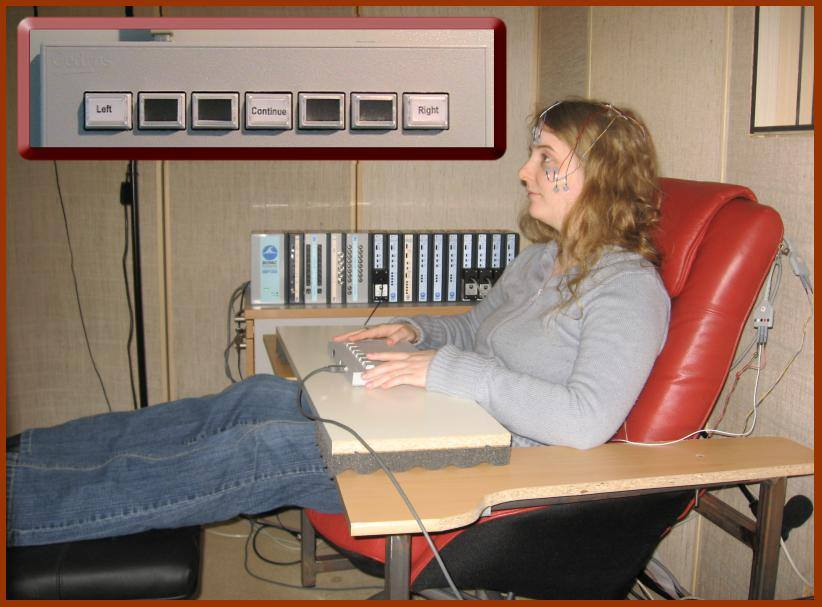
\includegraphics[width=0.65\textwidth]{./Psy/Kappas1.jpg}
    
    \caption{\itshape Facial activity is recorded using electromyography (EMG) while participant is watching emotional video clips. Inset shows the response box used to collect the responses of the participant. The experiment takes place in a sound-isolated box. Films are projected through a window from the neighboring control room.}%\label{fig:profxxx}
   \end{center}
\end{figure}

\begin{}
  \begin{center}
    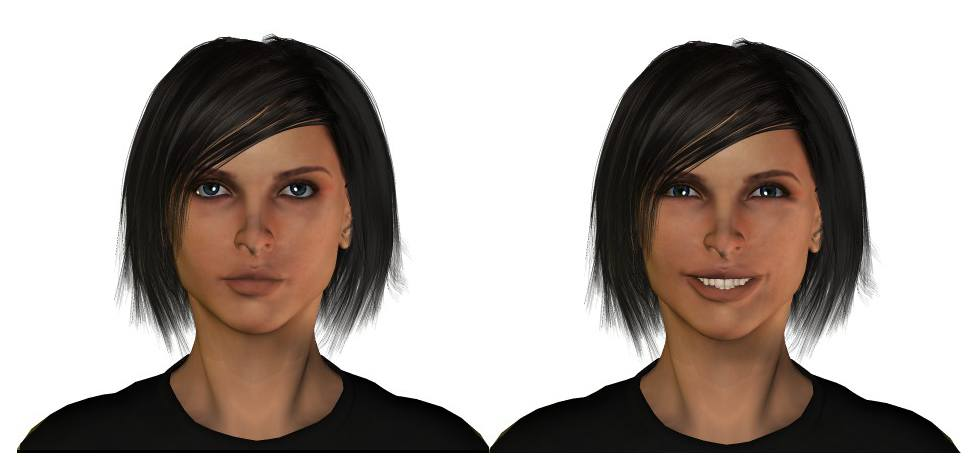
\includegraphics[width=0.8\textwidth]{./Psy/Kappas2.jpg}
    
    \caption{\itshape These faces were created using POSER 6 software (e frontier) and are used to study, for example, the role of temporal aspects of facial displays in person and expression perception.}%\label{fig:profxxx}
   \end{center}
\end{figure}

\vspace{0.6cm}


\vspace{0.6cm}
\textbf{Other Professional Activities}\\[-0.25cm]
\begin{enumerate}
\item[$\bullet$] Associate editor of Biological Psychology (Elsevier)
\item[$\bullet$] Member of editorial board of Journal of Nonverbal Behavior (Springer)
\item[$\bullet$] Editorial board of advisors of Cognition and Emotion (Taylor \& Francis)
\item[$\bullet$] Editorial consultant for British Journal of Social Psychology (British Psychological Society)
\item[$\bullet$] Board of Advisors The Centre for the Study of Emotion, University of Portsmouth
\item[$\bullet$] Reviews for further numerous journals as well as books.
\item[$\bullet$] Active member of several international scientific organizations; Charter member of the Association for Psychological Science, Fellow of the International Organization for Psychophysiology.
\end{enumerate}


\vspace{0.6cm}
\textbf{PhD-Students}\\[-0.25cm]

Dennis K\"{u}ster\newline
\textit{Processes of Implicit and Explicit Sociality in Regulation of Emotional Displays}\\[-0.15cm]

\newpage
\subsection{Prof. Dr. Ulrich K\"{u}hnen }


\textbf{Main Research Interests}\\[-0.25cm]
\begin{enumerate}
\item[$\bullet$]	Self-concept and Social Information Processing 
\item[$\bullet$]	Cross-cultural Variations in Thinking, Feeling and Action
\item[$\bullet$]	Intercultural Understanding and Competence
\item[$\bullet$]	The Role of Cognitive Feelings in Judgment Formation
\end{enumerate}


\vspace{0.6cm}
\textbf{Research Activities}\\[-0.25cm]

Individuals can construe their identity either as an autonomous and independent entity or as being related to other people, thus stressing the interdependence with them. The differences in the way the self is defined have profound influences for the person's thinking, feeling and action. Understanding the exact mechanisms by which different self-views affect information processing is my most important research question. This research is closely related to cross-cultural studies, since it is a well-established finding that members of different cultural groups construe their identity primarily in either independent or interdependent terms. What is more, the individual construal of the self has been found to mediate the impact of culture on cognition in various domains. In 2006, Ulrich K\"{u}hnen extended this research in the following ways:
\begin{enumerate}
	\item[$\bullet$]While his previous research had focused primarily on the purely cognitive consequences of different self-views, most recently he started taking motivational implications of self-construals into account. Are independent and interdependent self-views related to approach and avoidance motivational states. What are the consequences of these states for independent or interdependent individuals? 
	\item[$\bullet$]Do the different self-views coincide with different agency concept and how do these differences attributions of observed and one's own behavior? Is the notion of free will more closely connected to independent rather than interdependent self-views?
\end{enumerate}
During the last year Ulrich K\"{u}hnen became more and more interested in applied aspects of Intercultural Psychology. This interest was partly fueled by the fact that he and his colleagues believe the multicultural IUB context offers great opportunities to study intercultural communication. Together they developed an initiative to improve intercultural understanding and competence on the IUB campus and beyond. This initiative includes intercultural workshops and trainings for IUB members, a new BA program, consultancy offers to external companies and accompanying applied research.

\vspace{0.6cm}



\textbf{Organization of Scientific Conferences}\\[-0.25cm]
\begin{enumerate}
\item[$\bullet$]	September 2006\newline
45. Kongress der Deutschen Gesellschaft f�r Psychologie\newline
N�rnberg\newline
Member of the Scientific Board  
\item[$\bullet$] September 2006\newline
International University Bremen \newline
Symposium on "Intercultural Understanding and Competence"\newline
funded by IUB
\end{enumerate}



\vspace{0.6cm}
\textbf{Other Professional Activities}\\[-0.25cm]
\begin{enumerate}
\item[$\bullet$] Chairman of the Social Psychology division (Fachgruppensprecher) of the Deutsche Gesellschaft f�r Psychologie
\item[$\bullet$] Member-at-large of the Executive Committees of the International Association for Cross-Cultural Psychology
\newpage
\item[$\bullet$] Together with Prof. Dr. Klaus Boehnke organizer (Head of the Local Organization Committee) of the $19^{\rm th}$ Congress of the International Association for Cross-Cultural Psychology in 2008 at IUB
\item[$\bullet$] Member of the Editorial Board of the journal \textit{Self \& Identity}
\item[$\bullet$] Ad hoc reviewer for the DFG, as well as for several scientific journals, including Personality and Social Psychology Bulletin; Psychological Science; Self and Identity
\end{enumerate}
\newpage
\subsection{Prof. Dr. Bettina Olk}


\textbf{Main Research Interests}\\[-0.25cm]
\begin{enumerate}
\item[$\bullet$]	Reflexive and Volitional Attention and their Dynamic Interaction
\item[$\bullet$]	Mechanisms of Saccadic Eye Movements and Target Selection
\item[$\bullet$]	Brain Mechanism Underlying Attention and Eye Movements
\item[$\bullet$]	Neuropsychological Syndromes: Spatial Neglect, Attention Disorders
\item[$\bullet$]	Special Populations: Attention in Autism Spectrum Disorders
\end{enumerate}


\vspace{0.6cm}
\textbf{Research Activities}\\[-0.25cm]

Orienting towards sources of information is a key prerequisite for an efficient interaction with our stimulus-rich environment. Reflexive orienting serves to guide attention very rapidly to areas of interest. Volitional orienting involves allocating attention in a goal-directed manner, e.g., based on the intention to attend to a specific stimulus. Depending on the stimuli and the task at hand, reflexive and volitional attention may be directed towards the same or opposing locations, the latter requiring the inhibition of reflexive orienting and the resolution of competition between reflexive and volitional factors. Bettina Olk's representative current projects investigate these kinds of orienting and how they interact, for example to control our eye movements. Many locations in our visual world potentially attract our attention and our gaze. But because we can only look at one point in space at a time, conflicts between candidate locations need be resolved. Current projects vary the demands on eye movement control and also aim at investigating the involvement of parietal and frontal cortex in such tasks by testing participants with brain injuries. Future studies (in collaboration with Prof. Hilgetag, IUB) will also apply Transcranial Magnetic Stimulation (TMS) to those brain areas to characterize their role. The research is conducted at IUB, at the University of Glasgow (with Dr. Monika Harvey) and the University of British Columbia (with Prof. Alan Kingstone). Further collaborations exist with several hospitals and rehabilitation centers in Bremen. A transdisciplinary research project (with Profs. Kappas and M�ller, IUB) investigates how different groups of people perceive press photography, how they interpret the visuals and how they react to them. The project is unique as it combines for the first time the methods of eye tracking (perception analysis), iconology (meaning interpretation) and psychophysiological measurement (emotional reaction).
\\
\begin{}
  \begin{center}
    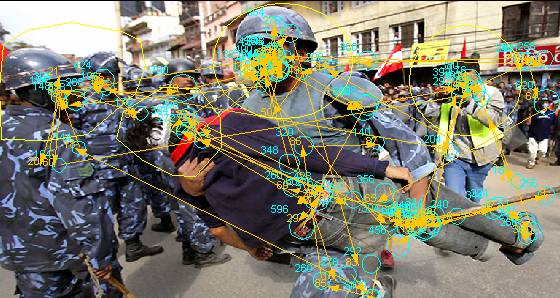
\includegraphics[width=0.8\textwidth]{./Psy/Olk.jpg}
    
    \caption{\itshape The picture shows a typical eye movement scanpath of a participant. Blue circles represent areas on which (and for how long) the participant fixated, yellow arrows illustrate eye movements.}%\label{fig:profxxx}
   \end{center}
\end{figure}


\newpage

\textbf{Funded Projects}\\[-0.25cm]
\begin{enumerate}
\item[$\bullet$]  "Integration of reflexive and volitional orienting: Comparing visual attention and eye movement control", in collaboration with Prof. Dr. Alan Kingstone, University of British Columbia, Canada, funded by the German Academic Exchange Service (DAAD)
\item[$\bullet$]  "Integration of reflexive and volitional orienting: Comparing motor systems", in collaboration with Dr. Monika Harvey, University of Glasgow, Scotland funded by The Royal Society
\end{enumerate}



\vspace{0.6cm}
\textbf{Other Professional Activities}\\[-0.25cm]
\begin{enumerate}
\item[$\bullet$] Reviewer for the following scientific journals: Experimental Brain Research, Journal of Experimental Psychology: Human Perception and Performance, Neuropsychologia, Perception, Perception \&
Psychophysics
\item[$\bullet$] Chair of the Academic Integrity Committee at IUB
\item[$\bullet$] Member of several international scientific organizations
\end{enumerate}


\vspace{0.6cm}
\textbf{Research Personnel}\\[-0.25cm]

Yu Jin\newline
Postdoctoral Fellow \\[-0.15cm]

\newpage
%Publications for History

%the function for the book publication could be as follows [it was not implemented here]
%1=author;2=year;3=title;4=publisher + comments
%\newcommand{\book}[4]{#1 (#2). \textit{#3}. #4}

\newpage

\subsection{Publications}




	\paragraph{Books} \textit{ }
	
\bigskip	


Dooley, B. (Ed.) (2006). \textit{Energy and culture: Perspectives on the power to work}. Burlington, VT: Ashgate. \\ 

Fischer-Tin\'{e}, H. (2006). \textit{Ausnahmezustand}. Novel by Nirmal Verma, translated from Hindi by H. Fischer-Tin\'{e}, \& H. Bauhaus-L\"{o}tzke. Heidelberg: Draupadi.\\ 

Frey, M. (2006). \textit{Dekolonisierung in S\"{u}dostasien. Die Vereinigten Staaten und die Aufl\"{o}sung der europ\"{a}ischen Kolonialreiche}. M\"{u}nchen: Oldenbourg.\\ 

Leutner, M., Spakowski, N., \& Yu, C.M. (Eds.) (2006). \textit{Gonghe shidai de Zhongguo fun\"{u} (Women in China. The Republican Period in Historical Perspective)}. Taipei: Rive Gauche Publishing, in press.\\ 

Paulmann, J. (2006). \textit{Die Haltung der Zur\"{u}ckhaltung: Ausw\"{a}rtige Selbstdarstellungen nach 1945 und die Suche nach einem erneuerten Selbst-verst\"{a}ndnis in der Bundesrepublik} (= Schriftenreihe der Wilhelm und Helene Kaisen-Stiftung), Bremen: Kaisen-Stiftung.\\ 

Spakowski, N., \& Milwertz, C. (Eds.) (2006). \textit{Women and gender in Chinese Studies. Special issue of Chinese History and Society/Berliner China-Hefte}, 29.\\ 



\paragraph{Articles \& Chapters}\textit{ }

\bigskip


Dooley, B. (2006). Art and information brokerage in the career of Don Giovanni de' Medici. In H. Cools, M. Keblusek, \& B. Noldus (Eds.), \textit{Your Humble Servant} (pp. 81-96). Hilversum: Verloren.\\ 

Fischer-Tin\'{e}, H. (2006). Global civil society and the forces of empire. The Salvation Army, British imperialism and the "pre-history" of NGOs. In S. Conrad, \& D. Sachsenmaier (Eds.), \textit{Conceptions of world order: Global historical approaches} (pp. 25-57). New York: Palgrave, in press.\\ 

Fischer-Tin\'{e}, H. (2006). Stadt der Pal\"{a}ste? - Europ\"{a}ische Lebenswelten im kolonialen Kalkutta. In R. Ahuja, \& C. Brosius (Eds.), \textit{Megast\"{a}dte in Indien: Mumbai, Delhi, Calcutta} (pp. 241-256). Heidelberg: Draupadi. \\ 

Fischer-Tin\'{e}, H. (2006). "Deep Occidentalism"? - Europa und der Westen in der Wahrnehmung hinduistischer Intellektueller und Reformer (ca. 1890-1930). \textit{Journal of Modern European History, 4}(2), 171-203.\\ 

Fischer-Tin\'{e}, H. (2006). From \textit{Brahmacharya} to conscious race culture: Indian nationalism, Hindu tradition and Victorian discourses of science. In C. Bates (Ed.), \textit{Beyond representation. The construction of identity in colonial India }(pp. 230-59). New Delhi: Oxford University Press.\\ 

Fischer-Tin\'{e}, H. (2006). Ananda Marga. In C. Auffahrt, H.-G. Kippenberg, \& A. Michaels (Eds.), \textit{W\"{o}rterbuch der Religionen }(p. 32). Stuttgart: Kr\"{o}ner.\\ 

Fischer-Tin\'{e}, H. (2006). Arya Samaj. In C. Auffahrt, H.-G. Kippenberg, \& A. Michaels (Eds.), \textit{W\"{o}rterbuch der Religionen }(p. 45). Stuttgart: Kr\"{o}ner.\\ 

Fischer-Tin\'{e}, H. (2006). Brahmo Samaj. In C. Auffahrt, H.-G. Kippenberg, \& A. Michaels (Eds.), \textit{W\"{o}rterbuch der Religionen }(p. 80). Stuttgart: Kr\"{o}ner.\\ 

Fischer-Tin\'{e}, H. (2006). Dayanand Sarasvati. In C. Auffahrt, H.-G. Kippenberg, \& A. Michaels (Eds.), \textit{W\"{o}rterbuch der Religionen }(p. 103). Stuttgart: Kr\"{o}ner.\\ 

Fischer-Tin\'{e}, H. (2006). Keshab Chandra Sen. In C. Auffahrt, H.-G. Kippenberg, \& A. Michaels (Eds.), \textit{W\"{o}rterbuch der Religionen} (p. 280). Stuttgart: Kr\"{o}ner.\\ 

Fischer-Tin\'{e}, H. (2006). Krishnamurti. In C. Auffahrt, H.-G. Kippenberg, \& A. Michaels (Eds.), \textit{W\"{o}rterbuch der Religionen} (p. 296). Stuttgart: Kr\"{o}ner.\\ 

Fischer-Tin\'{e}, H. (2006). Maharishi Mahesh Yogi. In C. Auffahrt, H.-G. Kippenberg, \& A. Michaels (Eds.), \textit{W\"{o}rterbuch der Religionen} (p. 318). Stuttgart: Kr\"{o}ner.\\ 

Fischer-Tin\'{e}, H. (2006). Neohinduismus. In C. Auffahrt, H.-G. Kippenberg, \& A. Michaels (Eds.), \textit{W\"{o}rterbuch der Religionen} (pp. 370-371). Stuttgart: Kr\"{o}ner.\\ 

Fischer-Tin\'{e}, H. (2006). Radhakrishnan. In C. Auffahrt, H.-G. Kippenberg, \& A. Michaels (Eds.), \textit{W\"{o}rterbuch der Religionen} (p. 419). Stuttgart: Kr\"{o}ner.\\ 

Fischer-Tin\'{e}, H. (2006). Rajneesh. In C. Auffahrt, H.-G. Kippenberg, \& A. Michaels (Eds.), \textit{W\"{o}rterbuch der Religionen} (p. 419). Stuttgart: Kr\"{o}ner.\\ 

Fischer-Tin\'{e}, H. (2006). Ramana Maharshi. In C. Auffahrt, H.-G. Kippenberg, \& A. Michaels (Eds.), \textit{W\"{o}rterbuch der Religionen} (p. 420). Stuttgart: Kr\"{o}ner.\\ 

Fischer-Tin\'{e}, H. (2006). Sri Aurobindo. In C. Auffahrt, H.-G. Kippenberg, \& A. Michaels (Eds.), \textit{W\"{o}rterbuch der Religionen} (p. 496). Stuttgart: Kr\"{o}ner.\\ 

Fischer-Tin\'{e}, H. (2006). Sundar Singh. In C. Auffahrt, H.-G. Kippenberg, \& A. Michaels (Eds.), \textit{W\"{o}rterbuch der Religionen} (p. 504). Stuttgart: Kr\"{o}ner.\\ 

Fischer-Tin\'{e}, H. (2006). Tagore (Debendranath). In C. Auffahrt, H.-G. Kippenberg, \& A. Michaels (Eds.), \textit{W\"{o}rterbuch der Religionen} (p. 509). Stuttgart: Kr\"{o}ner.\\ 

Fischer-Tin\'{e}, H. (2006). Tagore (Rabindranath). In C. Auffahrt, H.-G. Kippenberg, \& A. Michaels (Eds.), \textit{W\"{o}rterbuch der Religionen} (p. 509). Stuttgart: Kr\"{o}ner.\\ 

Fischer-Tin\'{e}, H. (2006). Vivekananda. In C. Auffahrt, H.-G. Kippenberg, \& A. Michaels (Eds.), \textit{W\"{o}rterbuch der Religionen} (p. 558). Stuttgart: Kr\"{o}ner.\\ 

Frey, M. (2006). Die Vereinigten Staaten und die Dritte Welt w\"{a}hrend des Kalten Krieges. In B. Greiner, \& D. Walther (Eds.), \textit{Hei�e Kriege im Kalten Krieg} (pp. 27-56). Hamburg: Hamburger Edition. \\ 

Frey, M. (2006). Zivilgesellschaft in historischer Perspektive: Die Niederlande und Deutschland im 19. Jahrhundert. \textit{Zentrum f\"{u}r Niederlande-Studien Jahrbuch f\"{u}r 2005, 16}, 11-32.\\ 

Frey, M. (2006). Mao Zedong. Nationalist und Despot. In S. F\"{o}rster, \& M. P\"{o}hlmann (Eds.), \textit{Kriegsherren der Weltgeschichte. 22 Historische Portraits} (pp. 357-372). M\"{u}nchen: C.H. Beck.\\ 

Spakowski, N., \& Milwertz, C. (2006). Introduction: Women and gender in Chinese Studies and the Women and Gender in Chinese Studies Network (WAGNet). In N. Spakowski, \& C. Milwertz (Eds.), \textit{Women and Gender in Chinese Studies}. Special issue of \textit{Chinese History and Society/Berliner China-Hefte, 29}, 3-4.\\ 

Spiekermann, U. (2006). From neighbour to consumer. The transformation of retailer-consumer relationships in twentieth-century Germany. In F. Trentmann (Ed.), \textit{The making of the consumer. Knowledge, power and identity in the modern world} (pp. 147-174). Oxford: Berg.\\ 

Spiekermann, U. (2006). Warum scheitert Ern\"{a}hrungskommunikation? In Aid e.V. (Ed.), \textit{Ern\"{a}hrungskommunikation. Neue Wege - neue Chancen?}. (pp. 11-20). Bonn: Aid.\\ 

Spiekermann, U. (2006). Warum scheitert die Ern\"{a}hrungskommunikation? Eine Antwort aus kulturwissenschaftlicher Perspektive. In E. Barl\"{o}sius, \& R. Rehaag (Ed.), \textit{Anforderungen an eine \"{o}ffentliche Ern\"{a}hrungskommunikation} (pp. 39-51). Berlin: Wissenschaftszentrum.\\ 

Spiekermann, U. (2006). Warenwelten. Die Normierung der Nahrungsmittel in Deutschland 1880-1930. In R.-E. Mohrmann (Ed.), \textit{Essen und Trinken in der Moderne} (pp. 99-124). M\"{u}nster: Waxmann.\\ 

Spiekermann, U. (2006). Brown bread for victory: German and British wholemeal politics in the interwar period. In F. Trentmann, \& F. Just (Ed.), \textit{Food and conflict in Europe in the age of the two World Wars} (pp. 143-171). Basingstoke: Palgrave Macmillan.\\ 

\newpage
%Lecture Talks for Psychology

\newpage  
\subsection{Invited Scientific Lectures and Talks}

{\hyphenpenalty=5000
\begin{flushleft}
January 2006\\[0.5cm]
\end{flushleft}
\begin{tabular}{lp{13.4cm}}
 Speaker:	&   Jens F\"{o}rster \\
 Place: 	 & Palm Springs, CA, USA\\
 Event:   &	Meeting of the Society for Personality and Social Psychology (SPSP) \\
 Title: &	Catharsis Revisited: Inhibition of Aggression-Related Constructs after Goal-Fulfillment (with Markus Denzler and Nira Liberman) \\ \\
\end{tabular}
\begin{tabular}{lp{13.4cm}}
 Speaker:	&   Jens F\"{o}rster \\
 Place: 	 & Palm Springs, CA, USA\\
 Event:   &	Meeting of the Society for Personality and Social Psychology (SPSP) \\
 Title: &	Abstract and Concrete Thinking: The Effects of Motivational Cues on Thinking Styles (with Stefanie Kuschel) \\ \\
\end{tabular}
\begin{tabular}{lp{13.4cm}}
 Speaker:	&   Jens F\"{o}rster \\
 Place: 	 & Palm Springs, CA, USA\\
 Event:   &	7th Annual Meeting of the Society for Personality and Social Psychology (SPSP)\\
 Title: &	Regulatory Focus and the Evaluation of Visual Arts - Implications for Motivational Effects on Attitudes (with Katrin Schimmel)\\ \\
\end{tabular}
\begin{tabular}{lp{13.4cm}}
 Speaker:	&   Jens F\"{o}rster \\
 Place: 	 & Palm Springs, CA, USA\\
 Event:   &	7th Annual Meeting of the Society for Personality and Social Psychology (SPSP)\\
 Title: &	Novelty Theory\\ \\
\end{tabular}
\begin{tabular}{lp{13.4cm}}
 Speaker:	&   Jens F\"{o}rster \\
 Place: 	 & Columbia University, New York, NY, USA\\
 Event:   &	Guest lecture\\
 Title: &	Novelty Theory\\ \\
\end{tabular}
\begin{tabular}{lp{13.4cm}}
 Speaker:	&   Jens F\"{o}rster \\
 Place: 	 & Bremen\\
 Event:   &	Conference "Jazzahead"\\
 Title: &	Zwischen Chaos und Sicherheit: Jazz als Modell einer balancierten Organisation mit innovativem Charakter\\ \\
\end{tabular}
\begin{tabular}{lp{13.4cm}}
 Speaker:	&   Jens F\"{o}rster \\
 Place: 	 &Zentrum f\"{u}r feministische Studien, Universit\"{a}t Bremen\\
 Event:   &	Guest lecture\\
 Title: &	Zur Sozialpsychologie der Vorurteile\\ \\
\end{tabular}
\begin{tabular}{lp{13.4cm}}
 Speaker:	&  	Ulrich K\"{u}hnen \\
 Place: 	 &Palm Springs, CA, USA\\
 Event:   &	7th Annual Meeting of the Society for Personality and Social Psychology (SPSP)\\
 Title: &	Consequences of Self-Regulatory Foci: Prevention Leads to Analytic Processing for Independents, but to Holistic Processing for Interdependents\\ \\
\end{tabular}
	

\newpage
\begin{flushleft}
February 2006\\[0.5cm]
\end{flushleft}
\begin{tabular}{lp{13.4cm}}
 Speaker:	&  Adele Diederich \\
 Place: 	 &Albert-Ludwigs-Universit\"{a}t Freiburg\\
 Event:   &	Freiburg Workshop of Diffusion Models\\
 Title: &		Diffusion Models for Multiattribute Choice Alternatives\\ \\
\end{tabular}
\begin{tabular}{lp{13.4cm}}
 Speaker:	&  Jens F\"{o}rster \\
 Place: 	 &M\"{u}nchen\\
 Event:   &	Forum 2006 der Trurnit Gruppe\\
 Title: &		Motivierte Mitarbeiter. Sozialpsychologische Erkenntnisse und Anwendungen\\ \\
\end{tabular}
	


\begin{flushleft}
March 2006\\[0.5cm]
\end{flushleft}
\begin{tabular}{lp{13.4cm}}
 Speaker:	&  Daniela Bockhorst \\
 Place: 	 &Mainz\\
 Event:   &	Tagung experimentell arbeitender Psychologen, TeaP\\
 Title: &		Personelle und situative Moderatoren riskanter Entscheidungen\\ \\
\end{tabular}
\begin{tabular}{lp{13.4cm}}
 Speaker:	&  Adele Diederich \\
 Place: 	 &T\"{u}bingen\\
 Event:   &	9. T\"{u}binger Wahrnehmungskonferenz\\
 Title: &		Why Two "Distracters" Are Better Than One: Modelling the Effect of Non-Target Auditory and Tactile Stimuli on Visual Saccadic Reaction Time\\ \\
\end{tabular}
\begin{tabular}{lp{13.4cm}}
 Speaker:	&  Adele Diederich \\
 Place: 	 &T\"{u}bingen\\
 Event:   &	9. T\"{u}binger Wahrnehmungskonferenz\\
 Title: &		Separating Multisensory Integration from Unspecific Warning Effects in Saccadic Reaction Time\\ \\
\end{tabular}
\begin{tabular}{lp{13.4cm}}
 Speaker:	&  Jens F\"{o}rster \\
 Place: 	 &Mainz\\
 Event:   &	Tagung experimentell arbeitender Psychologen, TeaP\\
 Title: &		Globale und lokale Wahrnehmung beeinflusst Assimilation und Kontrast bei sozialen Urteilen (with Stefanie Kuschel)\\ \\
\end{tabular}
\begin{tabular}{lp{13.4cm}}
 Speaker:	&  Jens F\"{o}rster \\
 Place: 	 &Mainz\\
 Event:   &	Tagung experimentell arbeitender Psychologen, TeaP\\
 Title: &		Fit macht Jungs attraktiv: Einfluss von regulatorischem Fit auf Personenbeurteilung (with Laura Dannenberg)\\ \\
\end{tabular}
\begin{tabular}{lp{13.4cm}}
 Speaker:	&  Jens F\"{o}rster \\
 Place: 	 &Mainz\\
 Event:   &	Tagung experimentell arbeitender Psychologen, TeaP\\
 Title: &		Odi et amo - Ich hasse und ich liebe. Der Einfluss von aggressiver und friedfertiger Zielerf\"{u}llung auf die Verf\"{u}gbarkeit von Aggression und auf aggressives Verhalten (with Markus Denzler and Nira Liberman)\\ \\
\end{tabular}
\begin{tabular}{lp{13.4cm}}
 Speaker:	&  Jens F\"{o}rster \\
 Place: 	 &Mainz\\
 Event:   &	Tagung experimentell arbeitender Psychologen, TeaP\\
 Title: &		Ann\"{a}herung und Vermeidung: Wie motivationale Faktoren Denkstile und die Enkodierung von Bedeutung und Details beeinflussen (with Stefanie Kuschel)\\ \\
\end{tabular}
\begin{tabular}{lp{13.4cm}}
 Speaker:	&  Rike Steenken \\
 Place: 	 &Oldenburg\\
 Event:   &	International Graduate School for Neurosensory Science and Systems\\
 Title: &		Multisensory Interaction: Unconscious Spatial Priming in an Audio-Visual Paradigm?\\ \\
\end{tabular}



\begin{flushleft}
April 2006\\[0.5cm]
\end{flushleft}
\begin{tabular}{lp{13.4cm}}
 Speaker:	&  Jens F\"{o}rster \\
 Place: 	 &Glocke, Bremen\\
 Event:   &	Sichtweisen in der Glocke\\
 Title: &		Tempo \& Termine - Wie die Zeit unser Leben bestimmt (with Bernhard Kramer)\\ \\
\end{tabular}
\begin{tabular}{lp{13.4cm}}
 Speaker:	&  Jens F\"{o}rster \\
 Place: 	 &Universit\"{a}t Dresden\\
 Event:   &	Universit\"{a}ts-Kolloquium\\
 Title: &		Die Psychologie der Gedankenunterdr\"{u}ckung\\ \\
\end{tabular}



\begin{flushleft}
May 2006\\[0.5cm]
\end{flushleft}
\begin{tabular}{lp{13.4cm}}
 Speaker:	&  Adele Diederich \\
 Place: 	 &Universit\"{a}t Osnabr\"{u}ck\\
 Event:   &	Workshop on Neuroscience and Neuroeconomics, FB Wirtschaftswissenschaften\\
 Title: &		Dynamic-Stochastic Models of Decision Making\\ \\
\end{tabular}
\begin{tabular}{lp{13.4cm}}
 Speaker:	&  Jens F\"{o}rster \\
 Place: 	 &Jena\\
 Event:   &	Socdoc meeting\\
 Title: &		Keynote Talk: Seven Principles of Self Regulation\\ \\
\end{tabular}
\begin{tabular}{lp{13.4cm}}
 Speaker:	&	Jens F\"{o}rster \\
 Place: 	 &Universiteit van Amsterdam, Netherlands\\
 Event:   &	Colloquium\\
 Title: &		New Perspectives on Social Psychology\\ \\
\end{tabular}
\begin{tabular}{lp{13.4cm}}
 Speaker:	&	Arvid Kappas \\
 Place: 	 &  Universit\�{e} Louvain-La-Neuve, Belgium \\
 Event:   &	2nd Meeting of the Consortium of European Research on Emotion (CERE)\\
 Title: &		Appraisal and Emotion Regulation (Keynote Address)\\ \\
\end{tabular}
\begin{tabular}{lp{13.4cm}}
 Speaker:	&	Arvid Kappas \\
 Place: 	 & Universit\�{e} Louvain-La-Neuve, Belgium\\
 Event:   &	2nd Meeting of the Consortium of European Research on Emotion (CERE)\\
 Title: &		Implicit Associations between the Concepts of Friends/Strangers with Showing/Hiding Emotions: An Indirect Investigation on the Relationship between Emotions and Expressions (with Dennis K\"{u}ster)\\ \\
\end{tabular}




\begin{flushleft}
June 2006\\[0.5cm]
\end{flushleft}
\begin{tabular}{lp{13.4cm}}
 Speaker:	&  Adele Diederich \\
 Place: 	 &Dublin, Ireland\\
 Event:   &	7th Annual Meeting of the International Multisensory Research Forum\\
 Title: &		Separating Multisensory Integration from Unspecific Warning Effects in Saccadic Reaction Time\\ \\
\end{tabular}
\begin{tabular}{lp{13.4cm}}
 Speaker:	&  Adele Diederich \\
 Place: 	 &Dublin, Ireland\\
 Event:   &	7th Annual Meeting of the International Multisensory Research Forum\\
 Title: &		Audio-Visual Integration of Letters and Speech: From Unimodal to Bimodal Subjective Representation\\ \\
\end{tabular}
\begin{tabular}{lp{13.4cm}}
 Speaker:	&  Adele Diederich \\
 Place: 	 &Dublin, Ireland\\
 Event:   &	7th Annual Meeting of the International Multisensory Research Forum\\
 Title: &		Visual-Tactile Integration: Does Stimulus Duration Influence the Relative Amount of Response Enhancement? (with Stefan Rach)\\ \\
\end{tabular}



\begin{flushleft}
July 2006\\[0.5cm] 
\end{flushleft}
\begin{tabular}{lp{13.4cm}}
 Speaker:	& Jens F\"{o}rster \\
 Place: 	 &M\"{u}nchen\\
 Event:   &	Tagung der Jungen Akademie\\
 Title: &		Keynote Talk: Wo bleibt die Zeit?\\ \\
\end{tabular}
\begin{tabular}{lp{13.4cm}}
 Speaker:	&  Jens F\"{o}rster \\
 Place: 	 &Kurt Lewin Institute, Groningen, Netherlands\\
 Event:   &	Kurt Lewin Workshop\\
 Title: &		KeynoteTalk: Seven Principles of Self Regulation\\ \\
\end{tabular}
\begin{tabular}{lp{13.4cm}}
 Speaker:	&  Jens F\"{o}rster \\
 Place: 	 &MPI Leipzig\\
 Event:   &	Colloquium\\
 Title: &		Solving Problems in a Social Context: The Motivational Underpinnings of Creative and Analytic Thinking\\ \\
\end{tabular}
\begin{tabular}{lp{13.4cm}}
 Speaker:	&  Arvid Kappas \\
 Place: 	 &University of Reading, England\\
 Event:   &	Psypag Annual Conference\\
 Title: &		Correlates of Hope: A Psychophysiological Perspective (with Malathy Rengamani and Sue Weaver)\\ \\
\end{tabular}
\begin{tabular}{lp{13.4cm}}
 Speaker:	&  Ulrich K\"{u}hnen \\
 Place: 	 &Universit\"{a}t Heidelberg\\
 Event:   &	Concluding Event of the "Experimentalpsychologisches Praktikum"\\
 Title: &	Kultur, Kontext und Kultur\\ \\
\end{tabular}
\begin{tabular}{lp{13.4cm}}
 Speaker:	&  Bettina Olk \\
 Place: 	 &Zurich, Switzerland\\
 Event:   &	Joint Meeting of the International Neuropsycholgical Society, Swiss Society of Neuropsychology, German Society of Neuropsychology\\
 Title: &	Volitional Orienting in Patients with Right-Hemisphere Lesions\\ \\
\end{tabular}
\begin{tabular}{lp{13.4cm}}
 Speaker:	&  Bettina Olk \\
 Place: 	 &M\"{u}nchen\\
 Event:   &	Colloquium of the Department of General Psychology, Ludwig-Maximilians-Universit\"{a}t M\"{u}nchen\\
 Title: &	Integration of Reflexive and Volitional Orienting\\ \\
\end{tabular}



\begin{flushleft}
August 2006\\[0.5cm] 
\end{flushleft}
\begin{tabular}{lp{13.4cm}}
 Speaker:	&  Adele Diederich \\
 Place: 	 &Vancouver, Canada\\
 Event:   &	39th Annual Society of Mathematical Psychology Meeting\\
 Title: &		Audiovisual Integration of Letters and Speech: A Fechnerian Scaling Analysis\\ \\
\end{tabular}
\begin{tabular}{lp{13.4cm}}
 Speaker:	&  Adele Diederich \\
 Place: 	 &Vancouver, Canada\\
 Event:   &	39th Annual Society of Mathematical Psychology Meeting\\
 Title: &		Modeling the Effects of Payoffs on Response Bias in a Perceptual Discrimination Task\\ \\
\end{tabular}
\begin{tabular}{lp{13.4cm}}
 Speaker:	&  Adele Diederich \\
 Place: 	 &University of Surrey, Guildford, England\\
 Event:   &	Workshop on Biologically Inspired Information Fusion\\
 Title: &		Distance From Discriminability: A Fechnerian Scaling Approach to Multisensory Integration\\ \\
\end{tabular}
\begin{tabular}{lp{13.4cm}}
 Speaker:	&  Arvid Kappas \\
 Place: 	 &Dartmouth College, New Hampshire, USA\\
 Event:   &	Minary Conference in Honor of Robert E. Kleck\\
 Title: &		People in Interaction: In their Muscles and their Brains!\\ \\
\end{tabular}





\begin{flushleft}
September 2006\\[0.5cm]
\end{flushleft}
\begin{tabular}{lp{13.4cm}}
 Speaker:	&  Adele Diederich \\
 Place: 	 &Brest, France\\
 Event:   &	37th European Mathematical Psychology Group meeting\\
 Title: &		A Fechnerian Analysis of Visual-Auditory Integration\\ \\
\end{tabular}
\begin{tabular}{lp{13.4cm}}
 Speaker:	&  Jens F\"{o}rster \\
 Place: 	 &N\"{u}rnberg\\
 Event:   &	45th Congress of the Deutsche Gesellschaft f\"{u}r Psychologie (DGPs)\\
 Title: &		Odi et amo - Ich hasse und ich liebe. Der Einfluss von aggressiver und friedfertiger Zielerf\"{u}llung auf die Verf\"{u}gbarkeit von Aggression und auf aggressives Verhalten (with Markus Denzler and Nira Liberman)\\ \\
\end{tabular}
\begin{tabular}{lp{13.4cm}}
 Speaker:	&  Jens F\"{o}rster \\
 Place: 	 &N\"{u}rnberg\\
 Event:   &	45th Congress of the Deutsche Gesellschaft f\"{u}r Psychologie (DGPs)\\
 Title: &		Selbstregulation und Denkstile: Einfluss motivationaler Orientierungen auf die Enkodierung von Bedeutung und Details (with Stefanie Kuschel)\\ \\
\end{tabular}
\begin{tabular}{lp{13.4cm}}
 Speaker:	&  Jens F\"{o}rster \\
 Place: 	 &N\"{u}rnberg\\
 Event:   &	45th Congress of the Deutsche Gesellschaft f\"{u}r Psychologie (DGPs)\\
 Title: &		Der Einfluss regulatorischer Foki auf Einstellungen zu Kunst (with Katrin Schimmel)\\ \\
\end{tabular}
\begin{tabular}{lp{13.4cm}}
 Speaker:	&  Jens F\"{o}rster \\
 Place: 	 &N\"{u}rnberg\\
 Event:   &	45th Congress of the Deutsche Gesellschaft f\"{u}r Psychologie (DGPs)\\
 Title: &		Ann\"{a}herungs- und Vermeidungsmotivation beeinflusst Assimilation und Kontrast bei sozialen Urteilen (with R. Friedman)\\ \\
\end{tabular}
\begin{tabular}{lp{13.4cm}}
 Speaker:	&  Jens F\"{o}rster \\
 Place: 	 &Heidelberg\\
 Event:   &	Milieus of Creativity\\
 Title: &		Creativity in Context: the Social Psychology of Creativity\\ \\
\end{tabular}
\begin{tabular}{lp{13.4cm}}
 Speaker:	&  Jens F\"{o}rster \\
 Place: 	 &Pultusk, Poland\\
 Event:   &	8th European Social Cognition Network: Transfer of Knowledge Conference\\
 Title: &		Cathartic Effects Revisited. The Impact of Goals on Aggressive Thoughts and Aggressive Behavior (with Markus Denzler and Nira Liberman)\\ \\
\end{tabular}
\begin{tabular}{lp{13.4cm}}
 Speaker:	&  Arvid Kappas \\
 Place: 	 &Coventry University, England\\
 Event:   &	34th Annual Scientific Meeting of the British Association for Cognitive Neuroscience (formerly British Psychophysiology Society)\\
 Title: &		Individual Differences in Dispositional Hope in Relation to Cardiovascular Reactivity, Pain Perception and Stress Appraisals (with Malathy Rengamani and Sue Weaver)\\ \\
\end{tabular}
\begin{tabular}{lp{13.4cm}}
 Speaker:	&  Ulrich K\"{u}hnen \\
 Place: 	 &N\"{u}rnberg\\
 Event:   &	45th Congress of the Deutsche Gesellschaft f\"{u}r Psychologie (DGPs)\\
 Title: &		Selbstkonzept und freier Wille: Sind "wir" weniger frei als "ich?" (with Laura Dannenberg)\\ \\
\end{tabular}



\newpage
\begin{flushleft}
October 2006\\[0.5cm] 
\end{flushleft}
\begin{tabular}{lp{13.4cm}}
 Speaker:	&  Jens F\"{o}rster \\
 Place: 	 &Philadelphia, USA\\
 Event:   &	2006 Conference of the Society of Experimental Social Psychology (SESP)\\
 Title: &		Seven Principles of Self Regulation\\ \\
\end{tabular}
\begin{tabular}{lp{13.4cm}}
 Speaker:	&  Jens F\"{o}rster \\
 Place: 	 &Chicago, USA\\
 Event:   &	Colloquium Chicago Business School\\
 Title: &	Novelty Theory: Implications for Abstract and Concrete Processing Styles\\ \\
\end{tabular}
\begin{tabular}{lp{13.4cm}}
 Speaker:	&  Arvid Kappas \\
 Place: 	 &Vancouver, BC, Canada\\
 Event:   &	46th Annual Meeting of the Society for Psychophysiological Research\\
 Title: &		Priming "We" or "They" Affects Level of Orbicularis Oculi Activity in Response to Funny Films: An Investigation on the Relationship between Emotions and Facial Activity (with Dennis K\"{u}ster)\\ \\
\end{tabular}
\begin{tabular}{lp{13.4cm}}
 Speaker:	& Bettina Olk \\
 Place: 	 &Vancouver General Hospital Eye Care Center, Canada\\
 Event:   &	Invited talk\\
 Title: &	Mechanisms of Reflexive and Volitional Orienting\\ \\
\end{tabular}


\begin{flushleft}
November 2006\\[0.5cm]
\end{flushleft}
\begin{tabular}{lp{13.4cm}}
 Speaker:	&  Adele Diederich \\
 Place: 	 &Houston, TX, USA\\
 Event:   &	47th Annual Meeting of the Psychonomic Society\\
 Title: &		Audiovisual Integration of Letters and Speech: A Fechnerian Scaling Analysis\\ 
\end{tabular}
\begin{tabular}{lp{13.4cm}}
 Speaker:	&  Adele Diederich \\
 Place: 	 &Magdeburg\\
 Event:   &	SFB-Jahrestagung of Sonderforschungsbereich/TransRegio 31 "Das aktive Geh\"{o}r"\\
 Title: &		An Experiment on Audio-Visual Integration of Letters (with Stefan Rach)\\ \\
\end{tabular}
\begin{tabular}{lp{13.4cm}}
 Speaker:	&  Amina \"{O}zelsel \\
 Place: 	 &Glocke, Bremen\\
 Event:   &	Sichtweisen\\
 Title: &		S\"{u}�es Ja und bitteres Nein (with Franziska Deutsch)\\ \\
\end{tabular}
\begin{tabular}{lp{13.4cm}}
 Speaker:	&  Bettina Olk \\
 Place: 	 &International University Bremen\\
 Event:   &	Workshop Autismustherapie\\
 Title: &		Aufmerksamkeit und Lernen: Grundlagen\\ \\
\end{tabular}
\begin{tabular}{lp{13.4cm}}
 Speaker:	&  Bettina Olk \\
 Place: 	 &Houston, TX, USA\\
 Event:   &	Psychonomics\\
 Title: &		Rethinking Voluntary and Involuntary Spatial Attention (with Alan Kingstone and Jelena Ristic)\\ \\
\end{tabular}
	



\begin{flushleft}
December 2006\\[0.5cm] 
\end{flushleft}
\begin{tabular}{lp{13.4cm}}
 Speaker:	&  Bettina Olk \\
 Place: 	 &Klinikum Bremen-Ost\\
 Event:   &	6th Conference on Cognitive Neuropsychiatry\\
 Title: &		Eye Movement Patterns as a Sensitive Measure of Deficits in Autism\\ \\
\end{tabular}
\begin{tabular}{lp{13.4cm}}
 Speaker:	&  Rike Steenken \\
 Place: 	 &Oldenburg\\
 Event:   &	International Graduate School for Neurosensory Science and Systems\\
 Title: &	Does Spatial Audio-Visual Interaction Depend on Awareness of Acoustical Stimulus' Locations?\\ \\
\end{tabular}

}

\newpage
\section{Social Sciences}
\shorttitle{Social Sciences}
\subsection{Prof. Dr. Andreas Bausch}


\textbf{Main Research Interests}\\[-0.25cm]
\begin{enumerate}
\item[$\bullet$]	Strategic Management
\item[$\bullet$]	International Management
\item[$\bullet$]  Controlling
\item[$\bullet$]	Entrepreneurship
\end{enumerate}


\vspace{0.6cm}
\textbf{Research Activities}\\[-0.25cm]

Prof. Bausch's major research focus has been on evidence-based best practices in strategic management and is anchored in the Center for Management Studies (CMS) at IUB. With the explosion of information from empirical research over the past decades, evidence-based strategic management strives to synthesize and interpret the research findings available in the field. Meta-analysis is to date widely used almost exclusively in medicine and psychology, having set a benchmark there. In the CMS meta-analysis is used to generate theory, to identify emerging issues in the field, to examine controversial or complicated topics, and to explicate "how to" strategies for practitioners. So far, internationalization, innovation, diversification, alliance activities, and mergers and acquisitions have been found to have a significant impact on firm performance.
\begin{figure}[ht]
  \begin{center}
    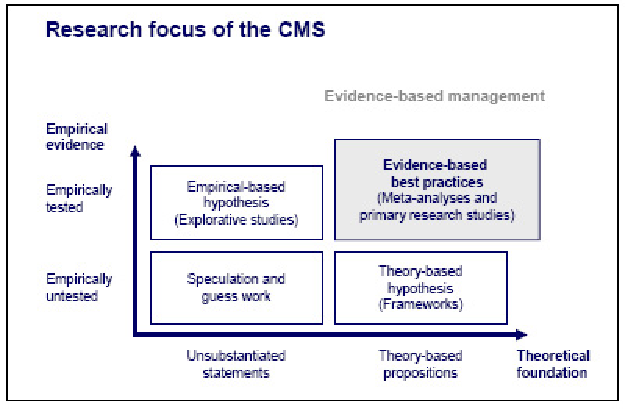
\includegraphics[width=0.7\linewidth]{./SocSci/Bausch-fig001.pdf}
%   \mycaption{ xxx )}\label{fig:profxxx}
   \end{center}
\end{figure}\\[-0.4cm]
After the success of the first two "Value Creator" studies (published in 2002 and 2004), a third study has been initiated together with Accenture. This study investigates the critical success factors of energy suppliers in Germany, Austria and Switzerland. In addition to accounting data from 1999 to 2005, this follow-up study will also be based on a management survey distributed to executives of utility companies. Together with The Advisory House AG a joint research funded by RWE AG analyzing demographic change in Europe and its impact on the labor market has been set-up. The overall aim of the study is not only to forecast the labor market in 2020 but also to develop comprehensive scenarios and to derive scenario specific recommendations for multinational corporations. Additionally, Prof. Andreas Bausch has submitted a research grant proposal on the antecedents and outcomes of radical vs. incremental innovation to the VolkswagenStiftung together with Profs. Michael Frese (Justus-Liebig-Universit�t Gie�en), James L. Farr (Penn State University), Shaker Zahra (University of Minnesota). The research team is planning to conduct a cross-cultural study on the influences of institutional, organizational, and psychological factors influencing radical and incremental innovation activity of firms in Germany and the US. 

\vspace{0.6cm}


\textbf{Funded Projects}\\[-0.25cm]
\begin{enumerate}
\item[$\bullet$]   Center for Management Studies - funded by The Advisory House AG
\item[$\bullet$]	 Empirical study "Value Creator III" - funded by Accenture GmbH
\item[$\bullet$]	 Empirical study "Demographic Change" - funded by RWE AG
\end{enumerate}


\vspace{0.6cm}
\textbf{Organization of Scientific Conferences}\\[-0.25cm]
\begin{enumerate}
\item[$\bullet$]	October 2006\newline
	Universit�t Bremen\newline
  "Unternehmertage 2006 - Der Mittelstand auf dem Weg ins Ausland"\newline
	funded by: PriceWaterhouseCoopers, Bremische Volksbank eG, 	Deutsche Bank, Bremer Landesbank, Commerzbank, Sparkasse 	Bremen 
\end{enumerate}


\vspace{0.6cm}
\textbf{Other Professional Activities}\\[-0.25cm]
\begin{enumerate}
\item[$\bullet$] Chair of Business Administration and International Management, School of Management and Economics, Friedrich Schiller Universit\"at Jena
\item[$\bullet$] Visiting Professor, Freie Universit\"at Bozen, Italy
\item[$\bullet$]	Academic Director of the Executive MBA Program in European Utility Management, International University Bremen
\item[$\bullet$]	Teaching of non-degree executive programs: amongst others for Deutsche Telekom, E.ON Academy, Salzgitter, and Delton
\end{enumerate}


\vspace{0.6cm}
\textbf{PhD-Students}\\[-0.25cm]

Kathrin B�secke\newline
\textit{Success Factors of Business Combinations}\\[-0.15cm]

Thomas Fritz\newline
\textit{Creating Superior Economic Performance through Sustainable Competitive Advantage}\\[-0.15cm]

Christian Grube\newline
\textit{The Valuation of Knowledge and Patents}\\[-0.15cm]

Mario Krist\newline
\textit{The Role of Intangible Resources in the Internationalization Process and their Contribution to Firm Performance}\\[-0.15cm]

Frithjof Pils\newline
\textit{Product Diversification and Corporate Financial Performance}\\[-0.15cm]

Nina Rosenbusch\newline
\textit{Antecedents and Outcomes of Radical vs. Incremental Innovation}\\[-0.15cm]

Duc Linh Van Tri\newline
\textit{Internationalization into the Chinese Market}



\vspace{0.6cm}
\textbf{Research Personnel}\\[-0.25cm]

Thomas Fritz\\[-0.15cm]

Duc Linh Van Tri
\newpage
\subsection{Prof. Dr. Matthijs Bogaards}


\textbf{Main Research Interests}\\[-0.25cm]
\begin{enumerate}
\item[$\bullet$]	Comparative Politics
\item[$\bullet$]	Democratization
\item[$\bullet$]	Political Parties
\item[$\bullet$]	Electoral Systems 
\item[$\bullet$]	Divided Societies
\end{enumerate}

\vspace{0.6cm}
\textbf{Research Activities}\\[-0.25cm]

In 2006, Matthijs Bogaards presented papers at various international conferences: at the tri-annual world conference of the International Political Science Association in Japan, at the annual meeting of the Swiss Political Science Association in Switzerland, and at a workshop in Institute Clingendael in the Netherlands organized by the hosts together with the United Nations University Tokyo and International IDEA of Stockholm. The topics of these papers reflect the wide ranging research interests of Matthijs Bogaards, which at the moment focus on the question of how to measure democracy and how to design democratic political institutions in divided societies. In 2006, Matthijs Bogaards finished three publications that will appear in international peer-reviewed political science journals in 2007. Following up on their successful workshop at the ECPR Joint Sessions in Granada in 2005 and two panels at the ECPR General Conference in Budapest later that year, Matthijs Bogaards and Fran�oise Boucek prepared an edited volume on \textit{Dominant Parties and Democracy}. A book proposal was submitted to Routledge. Finally, Matthijs Bogaards started writing a research monograph for Palgrave Macmillan with the title \textit{Democracy and Social Peace in Divided Societies: A Comparative Exploration of Power-Sharing Parties}. 


\vspace{0.6cm}
\textbf{Funded Projects}\\[-0.25cm]
\begin{enumerate}
\item[$\bullet$]	\textit{Managing Ethnic Conflict through Institutional Engineering: Ethnic Party Bans in Africa}\newline
(together with Dr. Matthias Basedau, Institut f�r Afrika-Kunde, 	Hamburg, Prof. Dr. Peter Niesen, Technical University Darmstadt, and 	Prof. Dr. Christoph Hartmann, University Bochum) \newline
funded by Thyssen Foundation
\end{enumerate}


\vspace{0.6cm}
\textbf{Other Professional Activities}\\[-0.25cm]
\begin{enumerate}
\item[$\bullet$]	Guest-editor of a special issue on 'Democracy and Power-Sharing in Multinational States' of the UNESCO \textit{International Journal of Multicultural Societies}, 8(2), 2006.
\item[$\bullet$]	Reviewer for \textit{European Journal of Political Research, Government \& 	Opposition, Journal of Politics, Journal of Theoretical Politics, Nations 	and Nationalism}
\item[$\bullet$]	Member of the Faculty Council at IUB
\end{enumerate}


\vspace{0.6cm}
\textbf{PhD-Students}\\[-0.25cm]

Sebastian Elischer \newline
\textit{Political Parties, Party Systems and Electoral Cleavages in Africa}
\newpage
\subsection[Prof. Dr. Hilke Brockmann]{Prof. Dr. Hilke Brockmann{\normalfont\normalsize\newline (Joined IUB in August 2006)}}


\vspace{0.3cm}
\textbf{Main Research Interests}\\[-0.25cm]
\begin{enumerate}
\item[$\bullet$]	Social Inequalities, Social Structure
\item[$\bullet$]	Life Course Research, Longitudinal Analysis
\item[$\bullet$]	Population Aging - Its Consequences for Modern States and Societies
\end{enumerate}


\vspace{0.6cm}
\textbf{Research Activities}\\[-0.25cm]

Hilke Brockmann's research in 2006 focused on three research questions: (a) Does population aging increase the demand for health care? (b) How much does a growing older population change the modern state? (c) And how much do policy changes feed back on social inequality? In order to answer the first question Hilke Brockmann conducted a study with colleagues from Universit�t Bremen analyzing health insurance data in order to investigate how health care reforms and health behaviour interact. Two papers have come out of this project so far, one in a peer-reviewed journal. Research concerning the second question is still at an early stage. Hilke Brockmann is currently writing a paper on "Governing generations" in which she compares family, migration and old-age policies in Germany and the US. She also started a small project on the "Demography of Political representatives" and prepared a grant application. Hilke Brockmann is about to finalize two papers one titled "Reforms that go under your skin. Health care and pension policy reform in Germany and the US" the other "Who care when singles die? Families and care at the end of life". Furthermore, a grant application on Health and Families is in preparation.
\begin{figure}[ht]
  \begin{center}
    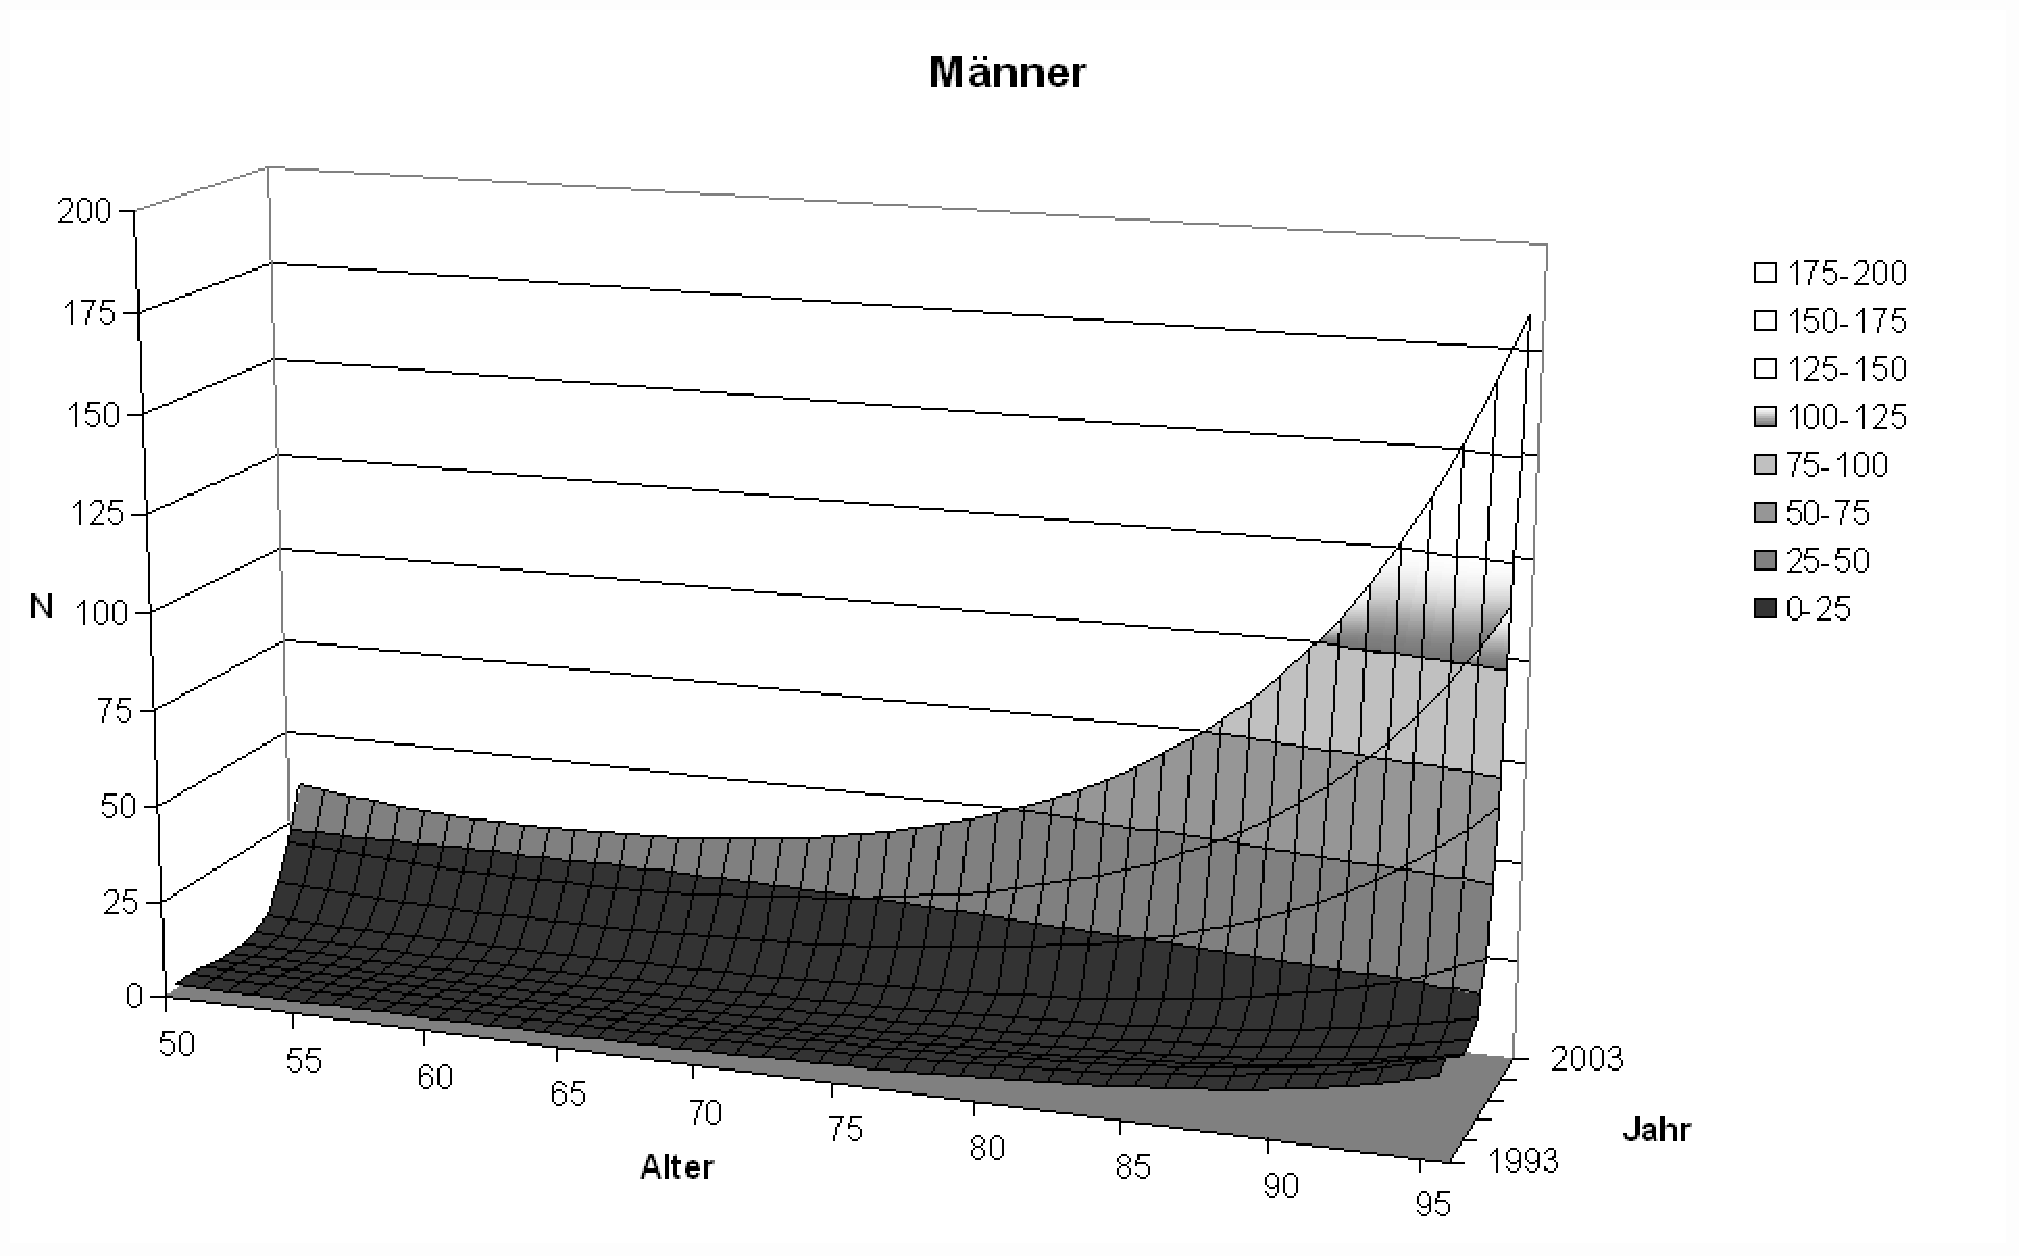
\includegraphics[width=0.95\linewidth]{./SocSci/Brockmann-fig001.pdf}
%   \mycaption{ xxx )}\label{fig:profxxx}
   \end{center}
\end{figure} 
\newpage
\begin{figure}[ht]
  \begin{center}
    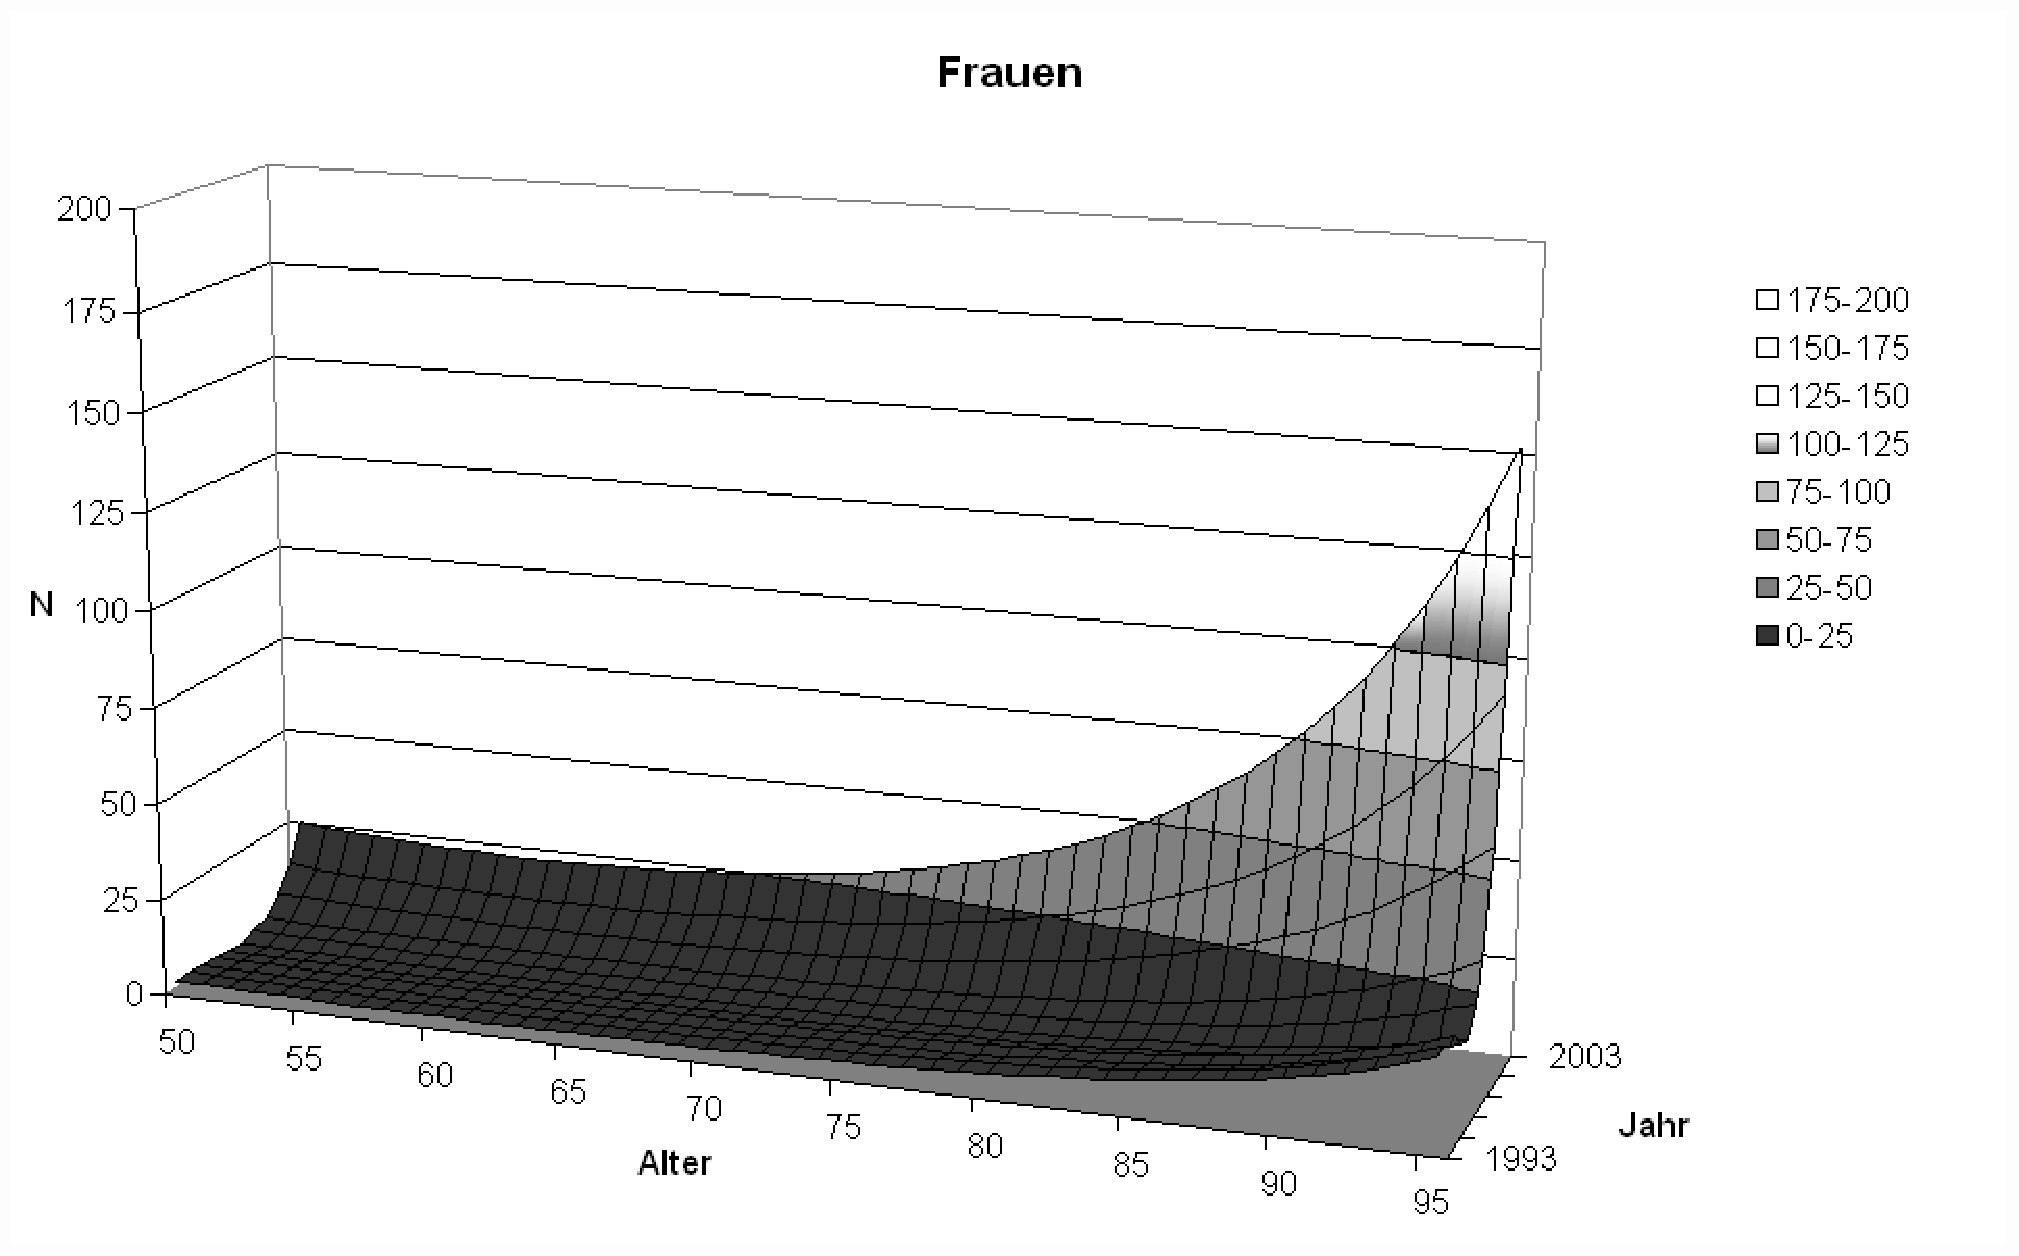
\includegraphics[width=0.95\linewidth]{./SocSci/Brockmann-fig002.pdf}
%   \mycaption{ xxx )}\label{fig:profxxx}
   \end{center}
\end{figure} 

\vspace{0.6cm}
\textbf{Funded Projects}\\[-0.25cm]
\begin{enumerate}
\item[$\bullet$]	Graduate School of Social Sciences (at Universit�t Bremen)
(together with Karin Gottschall, Steffen Mau, and Rainer Baumann),
funded by the VolkswagenStiftung
\end{enumerate}


\vspace{0.6cm}
\textbf{Other Professional Activities}\\[-0.25cm]
\begin{enumerate}
\item[$\bullet$]	Reviews for European Sociological Review
\item[$\bullet$]	Editorial Board of Health Sociology
\end{enumerate}


\vspace{0.6cm}
\textbf{PhD-Students}\\[-0.25cm]

Regine K�ller\newline
\textit{Verrentung = mehr Zeit = mehr Lebensqualit�t? Erwerbst�tigkeit und Zeiterfahrungen im Lebenslauf und die Auswirkungen auf die Gestaltung des Ruhestandes (retirement = more time = more quality of life? The impact of employment and time experience in the life course on the shaping of retirement)}\newline
Defense: March 2006\\[-0.15cm]

Bettina Kohlrausch\newline
\textit{A Ticket to Work? Active Labour Market Policy for the Young Unemployed in Britain and Germany}\\[-0.15cm]

Hao Yuan\newline
\textit{Social Development and Quality of Life: A Comparative Research Between Germany and China}\\[-0.15cm]

Oliver Horrmann\newline
\textit{ "Crowding in" versus "Crowding Out" - about the Impact of Different Welfare States on the Limits and Opportunities of the Provision of Family Care for the Elderly Generation}\\[-0.15cm]


\newpage
\subsection[Prof. Dr. Gert Brunekreeft] {Prof. Dr. Gert Brunekreeft{\normalfont\normalsize\newline(Joined IUB in September 2006)}}

\vspace{0.3cm}
\textbf{Main Research Interests}\\[-0.25cm]
\begin{enumerate}
\item[$\bullet$]	Competition Policy
\item[$\bullet$]	Economics of Regulation
\item[$\bullet$]	Industrial Organization
\item[$\bullet$]	Network Industries
\item[$\bullet$]	Electricity Markets
\end{enumerate}


\vspace{0.6cm}
\textbf{Research Activities}\\[-0.25cm]

In 2006 Gert Brunekreeft has been setting up a 2-year joint research project (jointly with a number of European universities where IUB takes the lead) on the pro's and con's of ownership unbundling of energy companies. This issue has high practical relevance and has only been studied poorly in the literature. Secondly he has engaged in research on the economic relation between different types of economic regulation of monopolies (like energy or railway networks) and investment in the infrastructure. This is a front issue in the academic debate, with significant economic relevance. Furthermore he has conducted research on the economics of regulation, eyeing in particular the design of incentive regulation for the German energy sector, as this should be implemented by January 1, 2008. As director of the Bremer Energie Institut, which is associated to IUB, Gert Brunekreeft--jointly with the colleagues at the institute--does research in energy-related environmental economics and policy. Hereby, the cost effective supply of combined heat and power and the energy efficiency both take pivotal roles. There are always a number of projects in process in the institute, funded by public bodies and industry alike.


\vspace{0.6cm}
\textbf{Funded Projects}\\[-0.25cm]

As Director of the Bremer Energie Institut (since September 1, 2006) Gert Brunekreeft was nominal principal investigator of the following funded research projects:
\begin{enumerate}
\item[$\bullet$]	"Investitionsanreize und die Randnummern 18 und 218 im Bericht der BNetzA nach �112a EnWG zur Einf�hrung der Anreizregulierung nach �21a EnWG."
\item[$\bullet$]	"Unbundling of Energy Companies: Is it worth it?"
\item[$\bullet$]	"Optimal networks"
\item[$\bullet$]	"Ermittlung von Effekten des KfW-CO2-Geb�udesanierungsprogramms"\newline
funded by KfW Bankengruppe, Frankfurt
\end{enumerate}


\vspace{0.6cm}
\textbf{Organization of Scientific Conferences}\\[-0.25cm]
\begin{enumerate}
\item[$\bullet$]	October 2006\newline
	Berlin\newline
	"5$^{\textrm{th}}$ Conference on Applied Infrastructure Research (INFRADAY)"\newline
	funded by: a number of sponsors, among them the European 	Commission.\newline
	international participants: 200  
\end{enumerate}


\vspace{0.6cm}
\textbf{Other Professional Activities}\\[-0.25cm]
\begin{enumerate}
\item[$\bullet$]	Senior Economist at EnBW AG Karlsruhe
\item[$\bullet$]	Director of the Bremer Energie Institut
\item[$\bullet$]	Co-editor of the journal \textit{Competition and Regulation in Network Industries} (CRNI)
\item[$\bullet$]	Research Fellow at a number of research institutions
\end{enumerate}


\vspace{0.6cm}
\textbf{Research Personnel}\\[-0.25cm]

As Director of the Bremer Energie Institut (since September 1, 2006) Gert Brunekreeft was nominal supervisor of the research associates at the Bremer Energie Institut (all of which are funded through diverse third-party grants).



\newpage
\subsection[Prof. Dr. Jan Delhey]{Prof. Dr. Jan Delhey{\normalfont\normalsize\newline (Joined IUB in September 2006)}}

\vspace{0.3cm}
\textbf{Main Research Interests}\\[-0.25cm]
\begin{enumerate}
\item[$\bullet$]	Social Inequality and Stratification
\item[$\bullet$]	Quality of Life and Subjective Well-being
\item[$\bullet$]	Social Capital and Trust
\item[$\bullet$]	Political Sociology of European Integration
\end{enumerate}


\vspace{0.6cm}
\textbf{Research Activities}\\[-0.25cm]

A first cluster of research activities of Jan Delhey was concerned with trust between European nations. On the one hand, the impact enlargements have had on the social cohesion of the European Union (EU), measured as generalized interpersonal trust between EU nationalities, has been explored. The key result is that enlargements do not necessarily weaken cohesion, but southern enlargement and the recent eastern enlargement did. The integrative effect of enlargement depends on the extent to which acceding nations differ from existing club members in three main dimensions: the level of modernization (mechanisms: prestige), cultural characteristics (mechanisms: similarity) and their power in the international system (mechanisms: perceived threat). On the other hand, the role of cross-border transaction for shaping trust in other nations has been explored. The main finding is that transactions are not key for trust in other nations. A second cluster of Jan Delhey's activities was concerned with life satisfaction. The main interest here was the effect of cross-border comparisons on individual happiness, which is a journey into unknown territory - the EU as a possible yardstick for national living conditions. Main findings are that large segments of EU-citizens are able to rate their country vis-�-vis EU average, and country-EU-comparisons are salient to life satisfaction - perceptions of deprivation or gratifications can make people more unhappy or more happy.


\vspace{0.6cm}
\textbf{Organization of Scientific Conferences}\\[-0.25cm]
\begin{enumerate}
\item[$\bullet$]	October 2006\newline
	Kassel\newline
	Congress of the Deutsche Gesellschaft f�r Soziologie (DGS)\newline
	Organizer of an ad hoc group "Sociology of European Integration"
\end{enumerate}


\vspace{0.6cm}
\textbf{Other Professional Activities}\\[-0.25cm]
\begin{enumerate}
\item[$\bullet$]	Board member of \textit{Journal of Happiness Studies}
\end{enumerate}\newpage
\subsection{Prof. Dr. Philipp Genschel}


\textbf{Main Research Interests}\\[-0.25cm]
\begin{enumerate}
\item[$\bullet$]	International Political Economy
\item[$\bullet$]	Transformations of the State in Advanced Capitalist Societies
\item[$\bullet$]	Tax Policy
\item[$\bullet$]	Theories of Institutions and Institutional Change
\end{enumerate}


\vspace{0.6cm}
\textbf{Research Activities}\\[-0.25cm]

Philipp Genschel has been involved in two main research activities in 2006. First, working on a joint project on international tax policy together with PhD students Thomas Rixen, Ingo Rohlfing and Susanne Uhl, he analysed the interaction between international governance institutions and state sovereignty in the field of taxation. Focusing on the global double tax treaty regime and the EU tax policy regime, he argues that the extensive guarantees these regimes provide for legal sovereignty in taxation paradoxically contribute to undermining national policy autonomy in this field. Research results will appear in a series of forthcoming papers in 2007. Second, in his capacity as deputy director of the Bremen Collective Research Center on the "Transformation of the State" (Sfb 597), he co-authored the Center's research program for 2007-2010. This research program was a key element of the Center's successful re-application for funding by the Deutsche Forschungsgemeinschaft in the fall of 2006.


\vspace{0.6cm}
\textbf{Funded Projects}\\[-0.25cm]
\begin{enumerate}
\item[$\bullet$]	"Der Steuerstaat und die internationale Steuerpolitik"\newline
	funded by the Deutsche Forschungsgemeinschaft as part of the 	Collaborative Research Center 597 "Transformations of the State"
\end{enumerate}

\vspace{0.6cm}
\textbf{Other Professional Activities}\\[-0.25cm]
\begin{enumerate}
\item[$\bullet$]	Deputy Director of the DFG Sonderforschungsbereich 597 "Staatlichkeit im Wandel" (Collaborative Research Center 597 "Transformations of the State")
\item[$\bullet$]	Co-Director MA International Relations (joint program of IUB and Uni Bremen)
\item[$\bullet$]	Director of IUB's Center for International Studies (CIS)
\item[$\bullet$]	Reviewer for several journals (including \textit{European Union Politics, European Journal for Political Research, European Journal of International Relations, Journal of Common Market Studies, Journal of European Public Policy}).
\item[$\bullet$]	Reviewer for the Deutsche Forschungsgemeinschaft
\end{enumerate}


\vspace{0.6cm}
\textbf{PhD-Students}\\[-0.25cm]

Junghoon Choi\newline
\textit{International Cooperation against Money Laundering and Tax Evasion: Similar Problems, Different Outcomes?}\\[-0.15cm]

Thomas Rixen\newline
\textit{The Political Economy of International Tax Cooperation: Institutional Choice and Development in International Taxation}\\[-0.15cm]

Ingo Rohlfing\newline
\textit{Trading Interests: Bilateralism and Multilateralism in International Trade Cooperation, 1860-2005}\\[-0.15cm]

Susanne Uhl\newline
\textit{Die Transformation von Steuerstaatlichkeit in Europa}


\vspace{0.6cm}
\textbf{Research Personnel}\\[-0.25cm]

Thomas Rixen, Ingo Rohlfing and Susanne Uhl work as research associates in the project "Der Steuerstaat und die internationale Steuerpolitik"
\newpage
\subsection[Prof. Dr. Markus Jachtenfuchs] {Prof. Dr. Markus Jachtenfuchs{\normalfont\normalsize\newline(Left IUB in July 2006)}}


\vspace{0.3cm}
\textbf{Main Research Interests}\\[-0.25cm]
\begin{enumerate}
\item[$\bullet$]	European Integration
\item[$\bullet$]	Transformation of the State
\item[$\bullet$]	International Governance
\end{enumerate}


\vspace{0.6cm}
\textbf{Research Activities}\\[-0.25cm]

In 2006, Markus Jachtenfuchs has been involved in three main research activities. First, within the Collaborative Research Center (CRC) on Transformations of the State (Sonderforschungsbereich Staatlichkeit im Wandel, 2003-2006), he has participated in implementing the overall research agenda of the CRC and preparing the next application round in September 2006. This included the coordination of research projects in four thematic fields (resources, legitimacy, rule of law, and intervention) and the preparation of joint publications from these projects which will appear in 2006. Second, he has directed a research project on "The Internationalization of the Monopoly of Force" within the CRC dealing with the internationalization of police activity. Third, he has continued writing on the findings and potential of a governance approach to European integration.


\vspace{0.6cm}
\textbf{Funded Projects}\\[-0.25cm]
\begin{enumerate}
\item[$\bullet$]	"The Internationalization of the Monopoly of Force,"\newline
	funded by the Deutsche Forschungsgemeinschaft as part of the CRC 	"Transformations of the State"
\end{enumerate}


\vspace{0.6cm}
\textbf{Other Professional Activities}\\[-0.25cm]
\begin{enumerate}
\item[$\bullet$]	Managing editor of reviewed book series "Weltpolitik im 21. Jahrhundert" (World Politics in the 21st century), edited by the International Relations Section of the German Political Science Association
\item[$\bullet$]	Member of scientific or editorial boards: Journal of International Relations and Development, Zeitschrift f�r internationale Beziehungen, Politique Europ�enne, Institut f�r europ�ische Politik, COST A 24 Action: The Social Construction of Threats
\item[$\bullet$]	Reviewer for professional journals:\textit{ Journal of European Public Policy, Journal of Common Market Studies, European Journal of International Relations, International Organization, Zeitschrift f�r Internationale Beziehungen, Journal of International Relations and Development, Politische Vierteljahresschrift}
\item[$\bullet$]	Reviewer for research grants: Deutsche Forschungsgemeinschaft, Fritz-Thyssen-Stiftung, Volkswagenstiftung, Austrian Ministry of Science
\item[$\bullet$]	Reviewer and selection committee member for professorships at various German universities
\item[$\bullet$]	Member of accreditation committee for accrediation agency ACQUIN
\item[$\bullet$]	Co-chair of MA in International Relations (joint program IUB-Uni Bremen)
\end{enumerate}


\vspace{0.6cm}
\textbf{PhD-Students}\\[-0.25cm]

Simon Dalferth\newline
\textit{ Police Cooperation in the EU. Efficiency versus Civil Liberties}\\[-0.15cm]

Eva Herschinger\newline
\textit{ Understanding Security Policy and its Role for Identity Construction - an Analysis of the French Security Discourse}\\[-0.15cm]

Christiane Kasack\newline
\textit{ EU Justice and Home Affairs and the Transformation of the State}\\[-0.15cm]

Akos Kopper\newline
\textit{ The Meaning of Sovereignty in Immigration-related Issues among the EU and its Neighbours}\\[-0.15cm]

Moritz Wei�\newline
\textit{ Preferences and Institutional Settings. The European Union's Security Policy since the mid-1990s}


\vspace{0.6cm}
\textbf{Scientific Personnel}\\[-0.25cm]

Dr. J�rg Friedrichs\newline
Post doctoral researcher in the CRC project on "The Internationalization of the Monopoly of Force"

\newpage
\subsection[Prof. Dr. Christian Joppke] {Prof. Dr. Christian Joppke{\normalfont\normalsize\newline(Left IUB in July 2006)}}

\vspace{0.3cm}
\textbf{Main Research Interests}\\[-0.25cm]
\begin{enumerate}
\item[$\bullet$]	Immigration and Citizenship
\item[$\bullet$]	Ethnic Diversity Laws and Policies in Europe
\item[$\bullet$]	Institutional Accommodation of Islam in Europe and North America
\end{enumerate}


\vspace{0.6cm}
\textbf{Research Activities}\\[-0.25cm]

Between 1 January and 31 July 2006, Christian Joppke finished a research proposal, "Transformation of Citizenship in the Postnational State", for Collaborative Research Center "Transformations of the State" (directed by S. Leibfried and P. Genschel). It was favorably reviewed and suggested for inclusion in the CRC's request for follow-up funding from January 2008. In addition, Joppke finalized two articles, which he submitted for publication (outcome as yet pending). Christian Joppke also participated in the preparation of the proposal for a Bremen International Graduate School for Social Sciences in the framework of the Excellence Initiative; in it he functioned as a theme coordinator.
\begin{figure}[ht]
  \begin{center}
    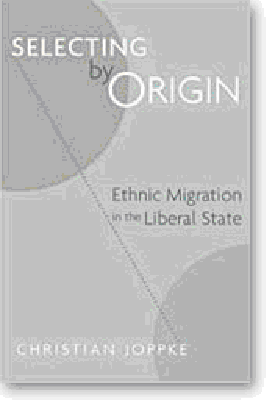
\includegraphics[width=5cm]{./SocSci/Joppke-fig001.pdf}
%   \mycaption{ xxx )}\label{fig:profxxx}
   \end{center}
\end{figure}


\vspace{0.6cm}
\textbf{PhD-Students}\\[-0.25cm]

Sara Geerdes\newline
\textit{Migration and Labor Market Transitions in selected European countries}
\newpage
\subsection{Prof. Dr. Peter Ludes}

\vspace{0.3cm}
\textbf{Main Research Interests}\\[-0.25cm]
\begin{enumerate}
\item[$\bullet$]	Mass Communication and Media Sociology, esp. Visual Communication
\item[$\bullet$]	Intercultural Comparisons
\item[$\bullet$]	Neglected News
\item[$\bullet$]	Sociology of Knowledge, Emotions, Time, Alternatives
\item[$\bullet$]	Theories of Civilizing Processes, Network Societies and Multiple Globalizations
\end{enumerate}


\vspace{0.6cm}
\textbf{Research Activities}\\[-0.25cm]

In 2006 Peter Ludes engaged (a) in the transdisciplinary study of media key visuals: The "flows of messages and images", which Manuel Castells saw as the "basic thread of our social structure", implying that "image-making is power-making", are seldom focused upon. Castells' theory of the "network society" therefore requires visual networks as illustrated by TV annual reviews of 2003-05;\\
\begin{figure}[ht]
  \begin{center}
    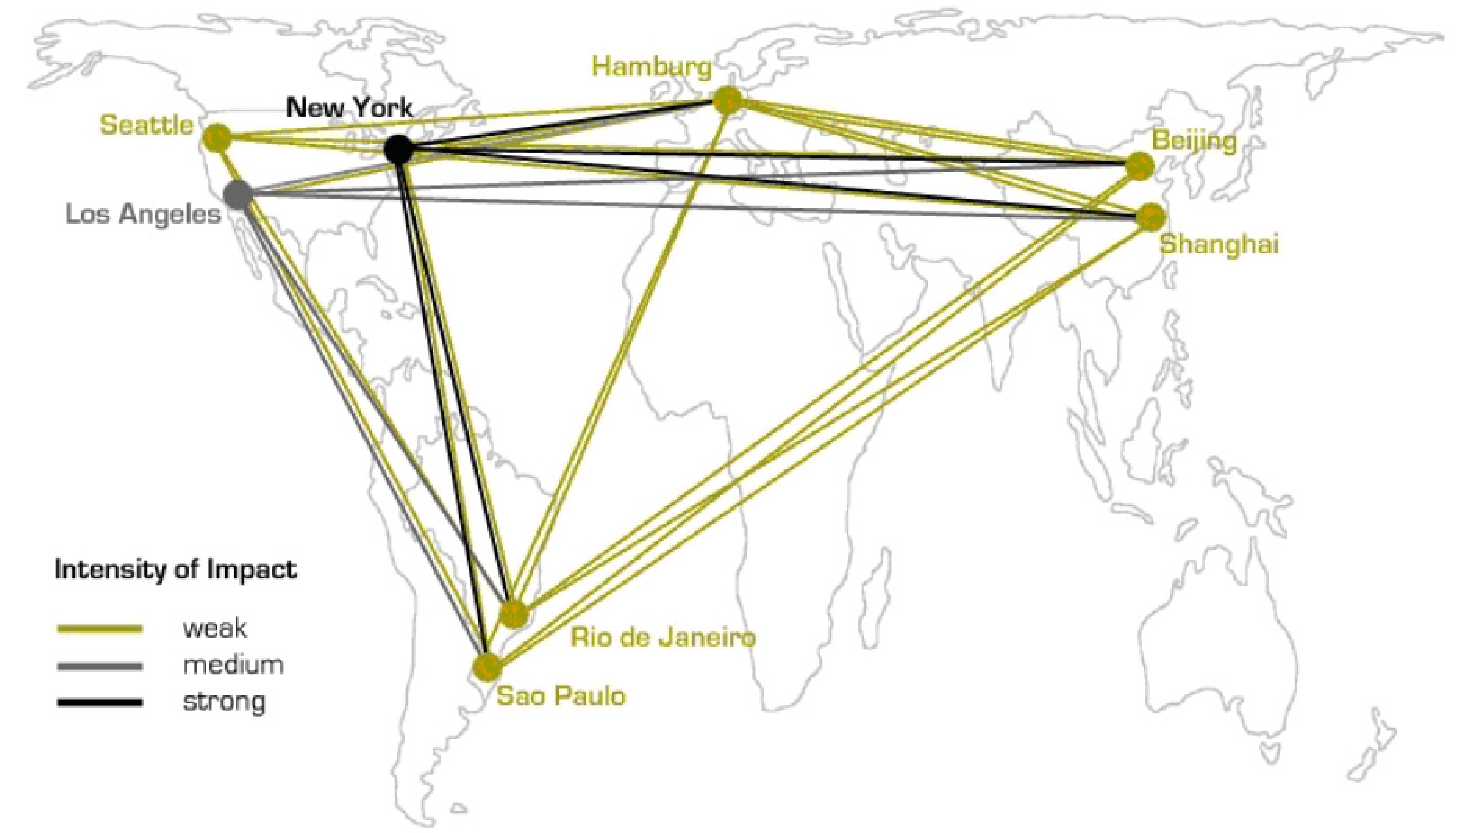
\includegraphics[width=\linewidth]{./SocSci/Ludes-fig001.pdf}
%   \mycaption{ xxx )}\label{fig:profxxx}
   \end{center}
\end{figure} 


(b) as deputy chair of the Research Network "Mass Media and Communication" of the European Sociological Association, current research on the interdependencies of techno-economic, political, and cultural developments with media formatting and contents was discussed in our e-mail network and at our conference in November 2006;
\newpage
\begin{figure}[ht]
  \begin{center}
    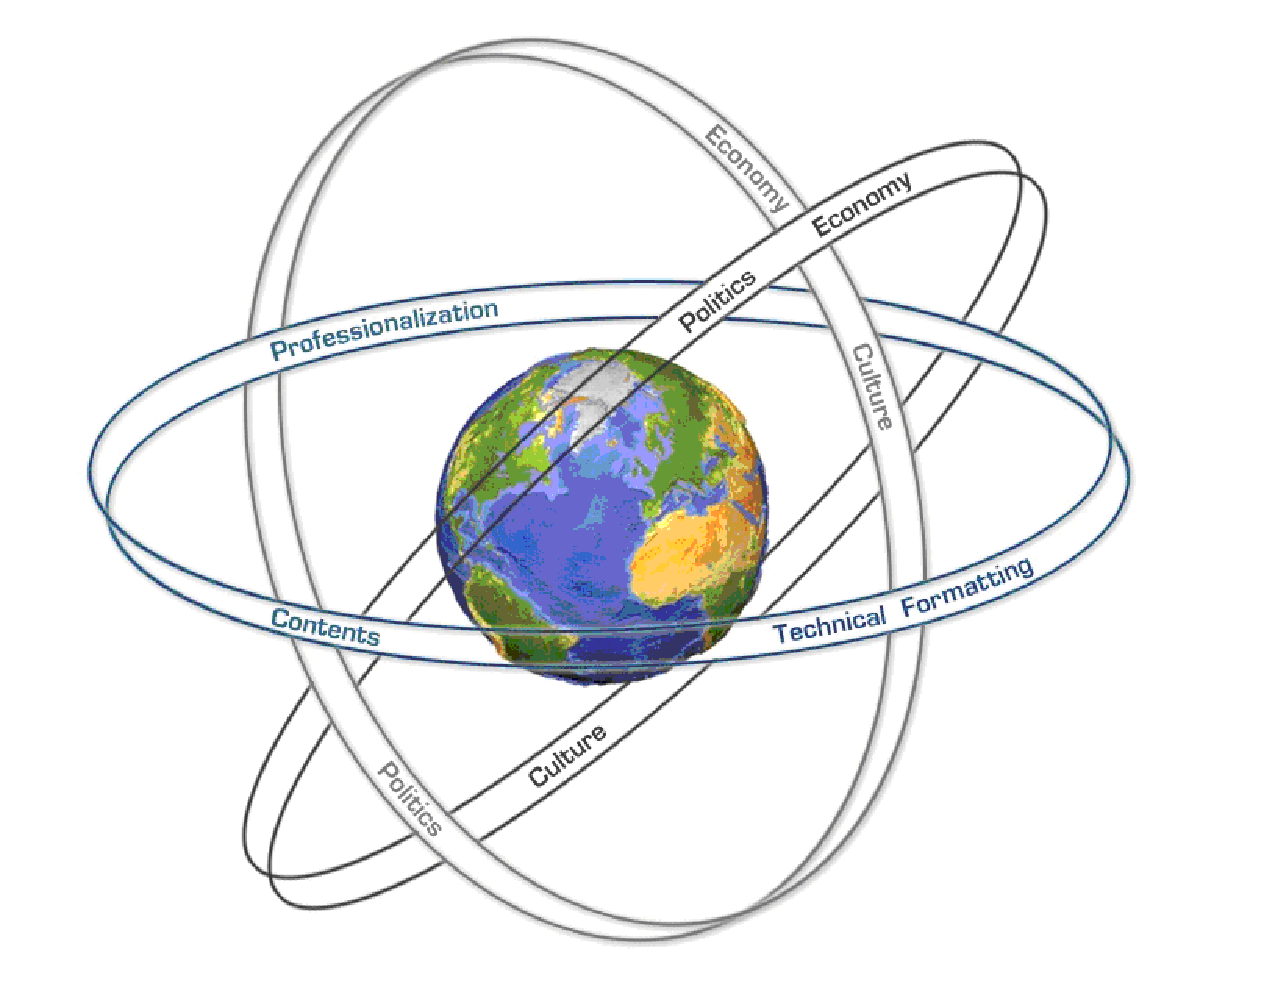
\includegraphics[width=0.8\linewidth]{./SocSci/Ludes-fig002.pdf}
%   \mycaption{ xxx )}\label{fig:profxxx}
   \end{center}
\end{figure}

(c) in the initiative "News Enlightenment" on neglected news in Germany, which he had founded in 1997, published the most neglected news of 2005 in February 2006 and has recruited new members for its jury.


\vspace{0.6cm}
\textbf{Organization of Scientific Conferences}\\[-0.25cm]
\begin{enumerate}
\item[$\bullet$]	January 2006\newline
International University Bremen\newline
Modelling and Decoding of Key Visuals in Intercultural Comparisons\newline
funded by IUB\\[-0.15cm]

\item[$\bullet$]	November 2006\newline
Antalya, Turkey\newline
Current Research\newline
funded by the European Sociological Association's Mass Media and Communications Research Network and Ankara University\newline
international participants: 15
\end{enumerate}


\vspace{0.6cm}
\textbf{Other Professional Activities}\\[-0.25cm]
\begin{enumerate}
\item[$\bullet$]	Deputy chair of the Research Network "Mass Media and Communications" of the European Sociological Association
\item[$\bullet$]	Speaker of an international group of researchers on Key Visuals
\item[$\bullet$]	Member of the task force of the International Communication Association on quality assessment
\item[$\bullet$]	External expert for the proposal for a Centre of Excellence in the Study of Democracy and the Digitisation of Audiovisual Culture (DIGICULT) of the University of Bergen
\item[$\bullet$]	Cooperation Partner for a Research Project on "Key Measures" of Prof. Dr. Leonardo Boccia, Federal University of Bahia, Salvador da Bahia, Brazil
\item[$\bullet$]	Member of the Jury of the Initiative Nachrichtenaufkl�rung \newline (www.nachrichtenaufklaerung.de) 
\item[$\bullet$]	Member of the Competence Center MultiMedia of the universities in Bremen state
\item[$\bullet$]	Referee for UK Economic and Social Research Council
\item[$\bullet$]	Member of the Research Development Committee of IUB
\end{enumerate}


\vspace{0.6cm}
\textbf{Research Personnel}\\[-0.25cm]

Christoph Kl�tsch\newline
Multimedia Research Fellow

\vspace{0.6cm}
\textbf{Guests}\\[-0.25cm]

Dr. Leonardo Boccia, Professor of Scenic Arts and Cultural Studies, Federal University of Salvador da Bahia (UFBA), funded by UFBA


\newpage
\subsection{Prof. Dr. Marion G. M�ller}

\vspace{0.3cm}
\textbf{Main Research Interests}\\[-0.25cm]
\begin{enumerate}
\item[$\bullet$]	Visual Communication
\item[$\bullet$]	The Use of Visuals in Times of War and Terrorism
\item[$\bullet$]	Visuals and Emotions
\item[$\bullet$]	Political Iconology
\item[$\bullet$]	Visual Competence
\item[$\bullet$]	Comparative Political Communication
\item[$\bullet$]	Symbolic and Ritual Communication
\item[$\bullet$]	Electoral Campaigns (US, Germany, EU)
\item[$\bullet$]	Comparative Parliamentary Studies
\end{enumerate}


\vspace{0.6cm}
\textbf{Research Activities}\\[-0.24cm]

Marion G. M�ller's major research activities in 2006 centered on further developing her visual archive: Politisch-ikonographisches Archiv der Vision (PIAV) with press-clippings and an image catalogue in both an electronic and in a printed postcard format. The archive is at the center of her current research interest in "Pathosformeln in den Massenmedien". Methodologically she applies the interpretative approach of political iconology in the tradition of the Kulturwissenschaftliche Bibliothek Warburg to the social sciences in an effort to make visual material accessible to the problem-oriented scrutiny of mass communication and political science. Her research questions center on the cohesion of democratic societies and the role of visuals in the process of creating and maintaining democratic belief systems. In this context she has devoted attention to the in-depth analysis of the cartoon conflict over Muhammad caricatures published by a Danish newspaper in late 2005 and eliciting violent responses in the Muslim world at the beginning of 2006. A second research focus, connected with the previously mentioned, is the use of images in times of war and terrorism, analyzing terrorist images published in the mass media and providing analyses of the ethical dilemma with which many journalists and editors are confronted in their decisions to publish images produced by terrorists. A third research focus in 2006 has been the scrutiny of perception and reception processes of press photography. The collaborative experimental study with her colleagues Professor Bettina Olk and Professor Arvid Kappas provides for a first and singular methodological combination of eye tracking, visual content analysis (iconology) and psychophysiological measurement of emotional reactions to press photography. The visual stimuli used in the first pilot experiment were violent protests in Nepal in spring 2006. Thus, this collaborative research project is additionally connected with Marion G. M�ller's interest in violent reactions to visuals. The theoretical framework for the collaborative study was formulated in an article published (with Arvid Kappas) in the peer-reviewed communication journal \textit{Publizistik} in spring 2006.

\vspace{0.6cm}
\textbf{Organization of Scientific Conferences}\\[-0.25cm]
\begin{enumerate}
\item[$\bullet$]	February 2006\newline
Hochschule f�r Philosophie, M�nchen\newline
"Bildethik" - Joint Annual Conference of the Visual Communication Division and the Division for Media and Communication Ethics of the DGPuK\newline
funded by Deutsche Gesellschaft f�r Publizistik und Kommunikationswissenschaft (DGPuK) and Hochschule f�r Philosophie M�nchen\newline
US-American keynote speaker
\end{enumerate}


\newpage
\textbf{Other Professional Activities}\\[-0.25cm]
\begin{enumerate}
\item[$\bullet$]	Chair of the Visual Communication Division of the German Communication Association (DGPuK)
\item[$\bullet$]	Vice Chair of the Visual Studies Division of the International Communication Association (ICA)
\item[$\bullet$]	Program Chair for organizing the Visual Studies Division's program for the Annual ICA Conference in San Francisco 2007
\item[$\bullet$]	Reviewer for the German Communication Association (DGPuK)
\item[$\bullet$]	Reviewer for the International Communication Association (ICA)
\item[$\bullet$]	Member of the adivsory board of the journal \textit{Politik \& Kommunikation}
\item[$\bullet$]	Member of the scientific advisory board of the Institut f�r Medienpolitik, Berlin
\item[$\bullet$]	Member of the DGPuK-"Selbstverst�ndnisausschuss"
\item[$\bullet$]	External member of the search committee for two W3 professorships "Kunstgeschichte" and "Kunst-Bildung-Vermittlung" at Universit�t Oldenburg
\item[$\bullet$]	Alumna 11$^{\textrm{th}}$ Transatlantic Forum (TAF), May 2006, BMW Stiftung Herbert Quandt
\end{enumerate}


\vspace{0.6cm}
\textbf{PhD-Students}\\[-0.25cm]

Ayse Esra �zcan\newline
\textit{Female Representation in Turkish Print Media}\\[-0.15cm]

Pinar Yildiz\newline
\textit{Honor Crimes and their Reception in the News}
\newpage
\subsection{Prof. Dr. Wolfgang Pfaffenberger}

\vspace{0.2cm}
\textbf{Main Research Interests}\\[-0.25cm]
\begin{enumerate}
\item[$\bullet$]	Energy Economics
\item[$\bullet$]	Electricity Economics
\item[$\bullet$]	Macroeconomic Aspects of Energy and Climate Policy
\item[$\bullet$]	Promotion of Energy Efficiency
\end{enumerate}


\vspace{0.5cm}
\textbf{Research Activities}\\[-0.25cm]

Network industries often display characteristics of a natural monopoly. Traditionally they were therefore organized as regional or local monopolies. In recent years in many parts of the world re-regulation took place by separating the bottleneck parts of the system (usually networks or parts of them) from the rest of the industry by various forms of regulation. For economists like Wolfgang Pfaffenberger it is of special interest to study the interaction between government regulation and the development of the markets and to review the regulatory concepts in light of the experience in the markets on the basis of empirical and modeling studies. At the same time the energy industry is a key sector for greenhouse gas reduction strategies. In this area a fundamental change of policy formation took place (international market for GHG certificates) on the basis of the global nature of GHG emissions whereas in the past direct intervention or taxation on the basis of national goals were dominant. It is of interest to observe this process of transformation. Economic models can serve as a basis for analyzing the rationale of policy making. Wolfgang Pfaffenberger undertakes research on this topic at Bremer Energie Institut within a multidisciplinary environment. Methods and approaches used depend on the subject of the project. In the first quarter of 2006 Wolfgang Pfaffenberger's research had was a focus on macroeconomic effects of renewable energy in connection with the "green roads to growth" conference. All projects are described in the annual report of the institute itself. The institute is an independent institute affiliated with Universit�t Bremen and IUB.


\vspace{0.6cm}
\textbf{Funded Projects}\\[-0.25cm]

As Director of the Bremer Energie Institut (until March 31, 2006) Wolfgang Pfaffenberger was nominal principal investigator of the following funded research projects:
\begin{enumerate}
\item[$\bullet$]	"Entwicklung des Endenergieverbrauchs f�r Heizung und Warmwasser bei Einfamilienh�usern,"\newline
funded by Bundesamt f�r Bauwesen und Raumordnung, Bonn
\item[$\bullet$]	"Ermittlung von Effekten des KfW-CO2-Geb�udesanierungsprogramms"
funded by KfW Bankengruppe, Frankfurt
\item[$\bullet$]	Implementation of Further-Education Measures on the topic of energy efficiency in buildings and "Energiepass"\newline
funded by EWE AG
\item[$\bullet$]	Coordination of the Bremer Contracting-Offensive\newline
funded by Bremer Energie-Konsens GmbH
\item[$\bullet$]	"Holzfeuerungsanlagen f�r Wohngeb�ude > 1000 m$^2$ Nutzfl�che"\newline
funded by Bundesamt f�r Bauwesen und Raumordnung (Bonn) and Bremer Energie-Konsens GmbH
\item[$\bullet$]	"Erfolgskontrolle des Einsatzes zentraler elektronischer Einzelraumremperaturregler in Wohnungen bez�glich der Akzeptanz und der Reduzierung des Energieverbrauchs"\newline
funded by Bremer Energie-Konsens GmbH
\item[$\bullet$]	"Analyses and Guidelines for Implementation of CHP Directive 2004/8/EC"\newline
funded by the European Commission, Directorate-General for Energy and Transport (GD TREN)
\item[$\bullet$]	Scientific evaluation of a model project on "Emissionshandel f�r Kleinverbraucher und Haushalte",\newline
funded by Landesinnungsverband des Schornseinfegerhandwerks Hessen
\end{enumerate}


\vspace{0.6cm}
\textbf{Organization of Scientific Conferences}\\[-0.25cm]
\begin{enumerate}
\item[$\bullet$]	June 2006\newline
Potsdam\newline
Annual international conference of the International Association for Energy Economics (IAEE)\newline
Member of the Program Committee
\end{enumerate}


\vspace{0.6cm}
\textbf{Other Professional Activities}\\[-0.25cm]
\begin{enumerate}
\item[$\bullet$]	Member of committee "Environmental and Resource Economics", Gesellschaft f�r Wirtschaftswissenschaften.
\item[$\bullet$]	Member of the board of "Gesellschaft f�r Energiewissenschaft und Energiepolitik (GEE)" (German branch of International Association for Energy Economics IAEE).
\item[$\bullet$] Kurzgutachten zu den Bestimmungsfaktoren der Gaspreise in Deutschland unter besonderer Ber\"ucksichtigung der Stadtwerke Auftraggeber: Ein Verbund norddeutscher Stadtwerk
\item[$\bullet$] Konzeption der energetischen Modernisierung eines Wohngebietes in Bremerhaven\newline Auftraggeber: Wohnungsgesellschaft ST\"AWOG Bremerhaven
\item[$\bullet$] Holzpelletheizsysteme f\"ur Ein-, Zwei- und kleine Mehrfamilienh\"auser - Technische Rahmenbedingungen und Wirtschaftlikeitsaspekte \newline Auftraggeber: Bremer Energie-Konsens GmbH
\item[$\bullet$] Detaillierung eines Konzepts zur Qualit\"atssicherung von Energieausweise \newline
Auftraggeber: F\"OGES F\"ordergemeinschaft f\"ur Geb\"aude- und Energiesysteme GmbH
\item[$\bullet$] Analyse des nationalen Potenzials f\"ur den Einsatz hocheffizienter KWK, einschlie�lich hocheffizienter Kleinst-KWK, unter Ber\"ucksichtigung der sich aus der EU-KWK-RL ergebenden Aspekte \newline
Auftraggeber: Bundesministerium f\"ur Wirtschaft und Arbeit
\item[$\bullet$] Qualit\"atssicherung Energieausweis: Gutachten zu Zielen, Nutzen, Instrumentarium und Methodik eines Systemes zur Qualit\"atssicherung von Energieausweisen \newline
Auftraggeber: Vereinigung der deutschen Zentralheizungswirtschaft e.V., Bonn
\item[$\bullet$] Einfluss des Heizsystems auf Schimmelpilze in  Wohnungen oder: Vermeiden Gasetagenheinzungen Schimmelpilze?
Auftraggerber: Bundesvereiningung der Firmen im Gas- und Wasserfach e.V. - figawa
\item[$\bullet$] Machbarkeitsstudie f\"ur eine Grasraffinerie\newline
Auftraggeber: Hanseatische Naturentwicklung GmbH (haneg)
\item[$\bullet$] Entwicklung des Endenergieverbrauchs f\"ur Heinzung und Warmwasser bei Einfamilienh\"ausern \newline
Auftraggeber: Bundesamt f\"ur Bauwesen und Raumordnung, Bonn
\end{enumerate}


\vspace{0.6cm}
\textbf{PhD-Students}\\[-0.25cm]

Stefanie Kesting\newline
\textit{Transmission Network Access Regulation in the European Gas Market}\newline
Defense: May 2006\\[-0.15cm]

Andres Ojeda\newline
\textit{Simulation Model for Electricity Pricing in a Market Environment}\newline
DAAD sandwich grant

\newpage
\vspace{0.6cm}
\textbf{Research Personnel}\\[-0.25cm]

As Director of the Bremer Energie Institut (until March 31, 2006) Wolfgang Pfaffenberger was nominal supervisor of the following research associates (all of which are funded through diverse third-party grants):\\[-0.2cm]

Dr.-Ing. Klaus-Dieter Clausnitzer\newline
Dr. rer. pol. J�rgen Gabriel\newline
Dr.-Ing. Bernd Eikmeier\newline
Dr. rer. nat. Karin Jahn\newline
Dipl.-Ing. Wolfgang Schulz\newline
Dipl.-Ing. Bernd Eikmeier
\newpage
\subsection{Prof. Dr. Dr. Dr. h.c. mult. Georg Ress}

\vspace{0.3cm}
\textbf{Main Research Interests}\\[-0.25cm]
\begin{enumerate}
\item[$\bullet$]	International Law
\item[$\bullet$]	Human Rights
\item[$\bullet$]	European Community Law (Conflicting Fundamental Rights, International Treaties)
\end{enumerate}


\vspace{0.6cm}
\textbf{Research Activities}\\[-0.25cm]

Georg Ress works predominantly of four particular law questions: First, the \textit{Interpretation of Art. 53 ECHR} and the so-called "Drittwirkung" of fundamental rights (since the judgment in the case Caroline von Hannover v. Germany the question has been asked, whether the EurCtHR should not leave a broader sphere of decision for the Constracting States , e.g.; balance between protection of privacy and freedom of press),. Georg Ress' research is concerned with the consequences of such an approach. Second, the \textit{Protection of Property} question of whether the restitution of property which was confiscated after the second world war under communist and socialist regimes are to be considered as a "special category." Third, the so-called \textit{Secret Treaties} collection of undisclosed international treaties, their legal effect and their observance compared with other treaties. And fourth, Diplomatic protection, encompassing a revision of lectures, given 2001 at the Academy of International Law in the Hague (in French). The last project which will take at least six months. Furthermore Georg Ress is working on an article about the interpretation of Art. 5, � 3 ECHR; conditions of release pending a trial.


\vspace{0.6cm}
\textbf{Other Professional Activities}\\[-0.25cm]
\begin{enumerate}
\item[$\bullet$]	Legal opinion for the Senate of Bremen on the financial claim against the Federation and other L�nder (financial emergency situation)
\item[$\bullet$]	Guest professor at the University of Kyoto
\item[$\bullet$]	Participation in the Conference on the European Internal Market concept, Vienna (Wien), president of one of the sessions
\item[$\bullet$]	Participation in several meetings of the former third section of the European Court of Human Rights, as its president, and of the Grand Chamber
\item[$\bullet$]	Participation in a meeting of the Commission on State Immunity and Human Rights of the Institute of International Law, London
\item[$\bullet$]	Invited expert: Bundestagsanh�rung, Menschenrechtsausschuss
\item[$\bullet$]	Participation in a meeting of the Reuters Founders Nomination Committee (member on behalf of the Council of Europe) in London
\item[$\bullet$]  Member of the Supervisory Board of the Saarbr\"ucker Zeitung Verlag und Druckerei GmbH
\end{enumerate}\newpage
\subsection[Dr. Jens Steffek] {Dr. Jens Steffek {\normalfont\normalsize\newline (Visiting Professor in Fall 2006)}}

\vspace{0.2cm}
\textbf{Main Research Interests}\\[-0.25cm]
\begin{enumerate}
\item[$\bullet$]	International Relations
\item[$\bullet$]	Global Governance
\item[$\bullet$]	World Society
\item[$\bullet$]	Political Theory
\end{enumerate}


\vspace{0.6cm}
\textbf{Research Activities}\\[-0.25cm]

In 2006 Jens Steffek has pursued two major research projects. First, he investigated emerging patterns of civil society participation in European and global governance. The aim of this comparative study of 32 international organizations/regimes is to evaluate whether enhanced participation by non-state actors can contribute to the democratic legitimacy of governance. Second, Jens Steffek studied mechanisms of global political redistribution, focusing on six policy areas beyond official development assistance.


\vspace{0.6cm}
\textbf{Funded Projects}\\[-0.25cm]
\begin{enumerate}
\item[$\bullet$]	"Legitimation and Participation in International Organizations", part of the Collaborative Research Centre "Transformations of the State", funded by the Deutsche Forschungsgemeinschaft (DFG)
\item[$\bullet$]	"The Role of Civil Society in Democratizing European and Global Governance", part of the integrated project "New Modes of Governance", funded by the European Commission under its 6$^{\textrm{th}}$ Framework Program
\end{enumerate}


\vspace{0.6cm}
\textbf{Organization of Scientific Conferences}\\[-0.25cm]
\begin{enumerate}
\item[$\bullet$]	October 2006\newline
International University Bremen\newline
"Staatlichkeit ohne Staat? Chancen und Aporien von Demokratie, Verfassung und Recht jenseits des Staates"\newline
(together with Dr. Nicole Deitelhoff, TU Darmstadt)\newline
funded within the framework of the Collaborative Research Centre "Transformations of the State"
\end{enumerate}


\vspace{0.6cm}
\textbf{Other Professional Activities}\\[-0.25cm]
\begin{enumerate}
\item[$\bullet$]	Referee for \textit{European Journal of International Relations, Journal of International Relations and Development, Millennium: Journal of International Studies, Political Studies, Zeitschrift f�r Internationale Beziehungen}
\item[$\bullet$]	Project reviewer for the Austrian Federal Ministry of Education, Science, and Culture (BMBWK)
\item[$\bullet$]	Reader for Oxford University Press
\end{enumerate}

\newpage
\subsection{Prof. Dr. Christian Welzel}

\vspace{0.3cm}
\textbf{Main Research Interests}\\[-0.25cm]
\begin{enumerate}
\item[$\bullet$]	Modernization and Social Change
\item[$\bullet$]	Democratization and Direct Democracy
\item[$\bullet$]	Value Formation and Value Change
\item[$\bullet$]	Human Development
\item[$\bullet$]	Protest Behavior and Social Movements
\item[$\bullet$]	Civil Society and Social Capital
\end{enumerate}


\vspace{0.6cm}
\textbf{Research Activities}\\[-0.25cm]

In recent years Christian Welzel has elaborated a concept of human development which allows analyzing the complex interrelations between the threefold process of economic modernization, cultural change, and democratization on a global scale. A major result of this research is the finding that economic modernization tends to give rise to emancipative cultural orientations, which in turn foster democracy if it already exists or make democracy more likely to emerge if it is not yet in place. 
Seen as a whole, this sequence reflects a broader process of human development in which economic modernization enables, rising emancipative values motivate, and more democracy allows people to pursue self-chosen preferences in their daily activities and lives at large (see Figure \ref{fig:Welzel002}). In the context of this interdisciplinary research, Welzel also helped to gather and to analyze data from the World Values Surveys in an attempt to specify the cultural orientations that are most conducive to honest government and democracy. These orientations have ultimately been identified and characterized as emancipative values (see Figure \ref{fig:Welzel001}).
\begin{figure}[ht]
  \begin{center}
    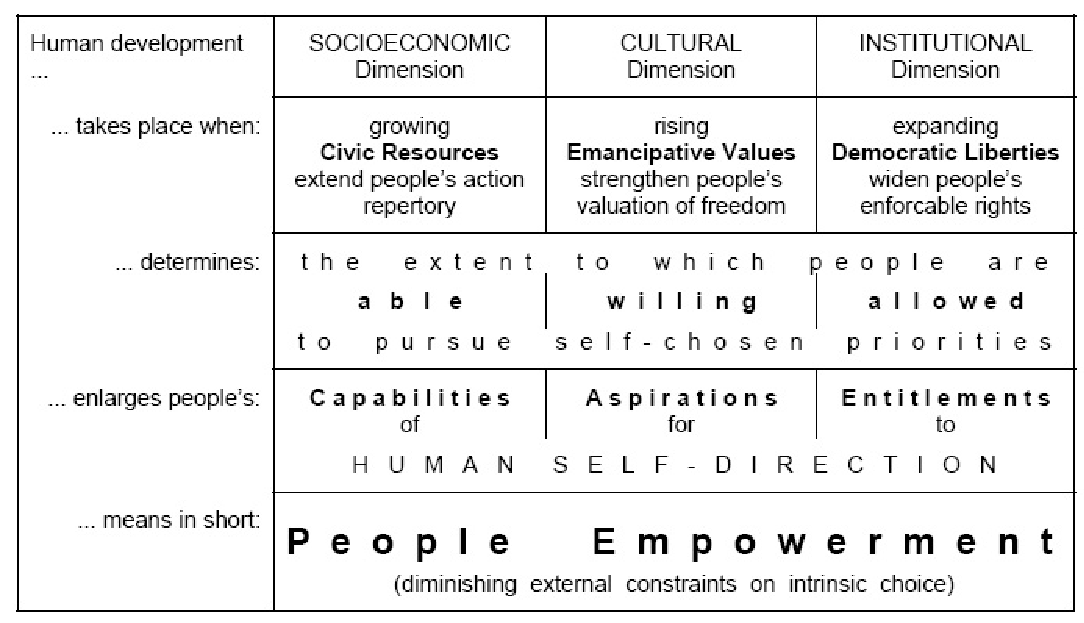
\includegraphics[width=\linewidth]{./SocSci/Welzel-fig002.pdf}
   \mycaption{\normalsize The Human Development of Societies \textit{Source:} Adapted from Welzel (2002:46).} 		  						\label{fig:Welzel002}
   \end{center}
\end{figure} 
\newpage
\begin{figure}[ht]
  \begin{center}
    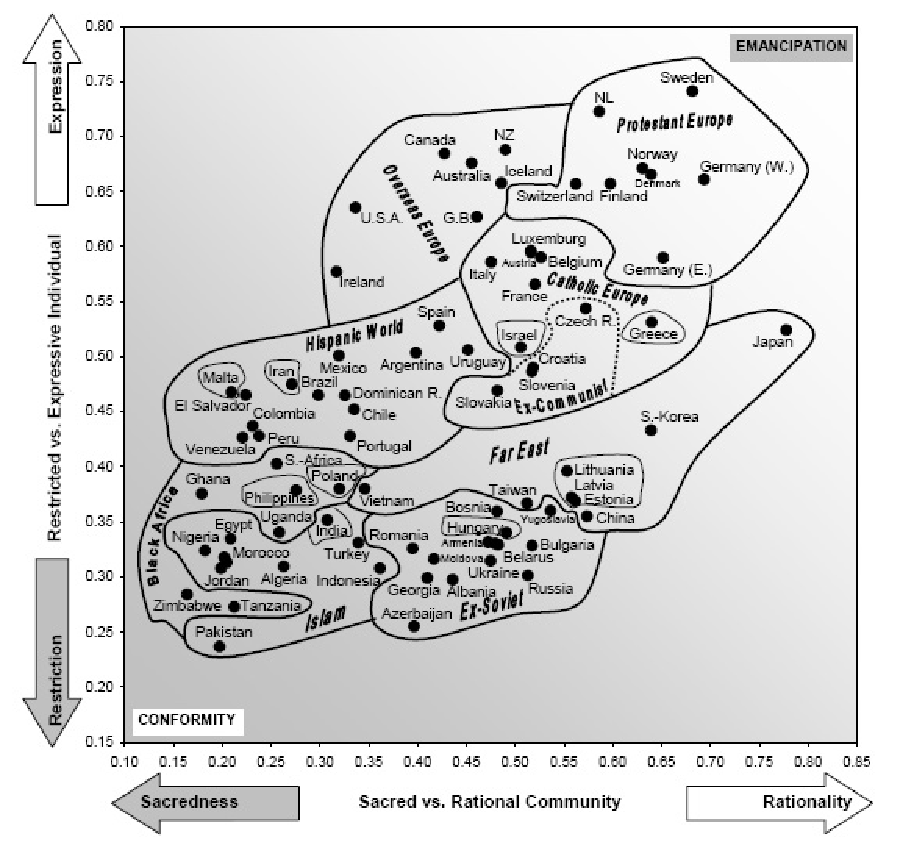
\includegraphics[width=0.9\linewidth]{./SocSci/Welzel-fig001.pdf}
   \mycaption{\normalsize Emancipative Values around the World} \label{fig:Welzel001}
   \end{center}
\end{figure} 


\textbf{Funded Projects}\\[-0.25cm]
\begin{enumerate}
\item[$\bullet$]	World Values Surveys: questionnaire design, coordinating fund raising activities and fieldwork, funded by Bank of Sweden Tercentenary Foundation
\item[$\bullet$]	German part of the World Values Surveys: principal investigator funded by Deutsche Forschungsgemeinschaft
\end{enumerate}


\vspace{0.6cm}
\textbf{Other Professional Activities}\\[-0.25cm]
\begin{enumerate}
\item[$\bullet$]	Member of the scientific advisory board of McKinsey company's "Perspektive Deutschland 2005"
\item[$\bullet$]	Consultant of the GfK's (Gesellschaft f�r Konsumforschung) study on value change
\item[$\bullet$]	Member of an expert group of the EU Commission on value orientations towards science and technology
\item[$\bullet$]	Member of scientific advisory board of the Telekom Foundation's "Innovationsindikator Deutschland"
\item[$\bullet$]	Member of the executive committee of the World Values Surveys Association
\item[$\bullet$]	IUB's official representative to the European Consortium of Political Science (ECPR)
\item[$\bullet$]	Co-organized several meetings of the executive committee of World Values Survey Association at various locations
\end{enumerate}


\newpage
\textbf{PhD-Students}\\[-0.25cm]

Alexander Boloussov\newline
\textit{Determinants of the Density of Human Rights NGOs in Postcommunist Publics}\\[-0.15cm]

Nicola B�cker\newline
\textit{Frames in European Identities in Postcommunist and Non-Postcommunist Publics}\\[-0.15cm]

Franziska Deutsch\newline
\textit{Participation and Democracy - Elite-Challenging Political Action in Old and New Democracies}\\[-0.15cm]

Jan M�ller\newline
\textit{The Influence of Values on the Interpretation of Collective Action Frames}\\[-0.15cm]

Yevgenya Paturyan\newline
\textit{Democratic Potential of Voluntary Associations in Semi-Democratic Postcommunist Regimes}\\[-0.15cm]

Caner Uguz\newline
\textit{Personality Cult in Politics: The Attat�rk Cult in Comparative Perspective}


\vspace{0.6cm}
\textbf{Research Personnel}\\[-0.25cm]

Franziska Deutsch works as research associate in the project "European and World Values Surveys" funded by the Deutsche Forschungsgemeinschaft


\newpage
\subsection{Prof. Dr. Welf Werner}

\vspace{0.3cm}
\textbf{Main Research Interests}\\[-0.25cm]
\begin{enumerate}
\item[$\bullet$]	International Monetary Regime Change
\item[$\bullet$]	International Trade in Services
\item[$\bullet$]	Trade Policy on Financial Services
\item[$\bullet$]	Regulation and Development of International Insurance Markets
\item[$\bullet$]	European Employment and Social Policies
\item[$\bullet$]	U.S. Economic Policy and Transatlantic Economic Relations
\item[$\bullet$]	History of Globalization
\item[$\bullet$]	U.S. Economic History
\end{enumerate}


\vspace{0.6cm}
\textbf{Research Activities}\\[-0.25cm]

Before joining IUB in 2004, Welf Werner worked in the fields of international economics, economic history, and U.S. economic policy. At IUB he has focused on Asia and particularly China, has engaged in a research project on European labor and social policies, and has broadened his interests in trade in services. Regarding international trade in services, Werner is interested in the compilation of trade statistics, the applicability of trade theory and in the ways and means of integrating services in regional and multilateral trade agreements. Topics covered in publications include welfare effects of services liberalization for developing countries, the status of liberalization commitments in the ongoing Doha negotiations at the World Trade Organization (co-authored with Walter Werner, the head of the German delegation in the Doha negotiations) and the conflicts created by trying to open financial markets while protecting the safety and soundness of national and international financial markets. With his work on European social and labor market policies, Werner crosses traditional academic boundaries. The VolkswagenStiftung is financing his research project "Globalization: Challenges for EU Social and Labor Market Policies" as part of its program "Welfare State Transformation: Bridging the Gap between Theory and Practice". While working at the Federal Ministry of Economics and Labor in Berlin for eight months Welf Werner advised on the European Employment Strategy (EES). After having focused on American and Atlantic policy issues at the Freie Universit�t Berlin, Harvard University and the School of Advanced International Studies of the Johns Hopkins University, Werner's shift of attention to Asia resulted in invitations to give presentations in Beijing and Seoul, supervision of a Chinese PhD student, and the publication of a paper on the rapid internationalization of Chinese financial markets in China's leading journal on international economics. Earlier interests, which Werner followed up with new papers, include the development of transatlantic merchandise trade and the dynamics of international reinsurance markets. 


\vspace{0.6cm}
\textbf{Funded Projects}\\[-0.25cm]
\begin{enumerate}
\item[$\bullet$]	"Globalization: Challenges for EU Social and Labor Market Policies," funded by VolkswagenStiftung in its program "Future Issues of our Society - Analysis, Advice and Communication between Academia and Practice. Welfare State Transformation: Bridging the Gap between Theory and Practice."
\end{enumerate}


\vspace{0.6cm}
\textbf{Organization of Scientific Conferences}\\[-0.25cm]
\begin{enumerate}
\item[$\bullet$]	March 2006\newline
Bonn\newline
"Jahrestagung of the Wirtschaftshistorischer Ausschuss, Verein f�r Socialpolitik"\newline
Member of the Scientific Board
\end{enumerate}


\vspace{0.6cm}
\textbf{Other Professional Activities}\\[-0.25cm]
\begin{enumerate}
\item[$\bullet$] Regular contributions of book reviews to \textit{Historische Zeitschrift, Vierteljahrschrift f�r Sozial- und Wirtschaftsgeschichte (VSWG)} and \textit{Harvard Business History Review}
\item[$\bullet$]	Referee for Studienstiftung des deutschen Volkes.
\item[$\bullet$]	Founding member of the Lions Club International University Bremen and the Center for International Studies, IUB.
\item[$\bullet$]	Member of Deutscher Hochschulverband, Wirtschaftshistorischer Ausschuss of the Verein f�r Socialpolitik, American Political Science Association, Verein f�r Unternehmensgeschichte, Verein f�r die gesamte Versicherungswissenschaft.
\item[$\bullet$]	Participating Researcher: Bremen International Graduate School of Social Sciences. Proposal for a Graduate School, Excellence Initiative by the German Federal and State Governments.
\item[$\bullet$]	Participating Researcher: Visual Hegemonies: Modeling and Decoding of Key Visuals in Intercultural Comparisons, IUB.
\item[$\bullet$]	Coordinator, Integrated Social Science Program, School of Humanities and Social Sciences, IUB. Together with Margrit Schreier.
\item[$\bullet$]	Consultant to the Federal Ministry of Economics and Labor, Berlin.
\end{enumerate}


\vspace{0.6cm}
\textbf{PhD-Students}\\[-0.25cm]

Okta Nofri\newline
\textit{Regional Integration: ASEAN and EU}
\newpage
\subsection{Prof. Dr. Hartmut Wessler}

\vspace{0.3cm}
\textbf{Main Research Interests}\\[-0.25cm]
\begin{enumerate}
\item[$\bullet$]	Comparative and Transnational Communication Research
\item[$\bullet$]	Intercultural Aspects of International Conflict Communication
\item[$\bullet$]	Theory of Public Discourse and the Public Sphere
\item[$\bullet$]	Political Communication
\item[$\bullet$]	Science and Risk Communication
\end{enumerate}


\vspace{0.6cm}
\textbf{Research Activities}\\[-0.25cm]

Hartmut Wessler is directing the project "The Transnationalization of Public Spheres: The Case of the EU" in the framework of the CRC "Transformations of the State". It investigates the Europeanization of national media coverage in five European countries since the 1980s. In Phase I of the project (2003-2006) the empirical patterns of Europeanization were investigated using a combination of quantitative and qualitative media content analysis. Patterns will be explained by studying the facilitating and constraining factors of Europeanization in Phase II of the project (2007-2010). Then the study will include Poland as a sixth country as well as tabloids in addition to quality newspapers. In Phase I the project has identified a complex pattern of "segmented and piecemeal Europeanization" in mediated public communication (see Figure)
\begin{figure}[ht]
  \begin{center}
    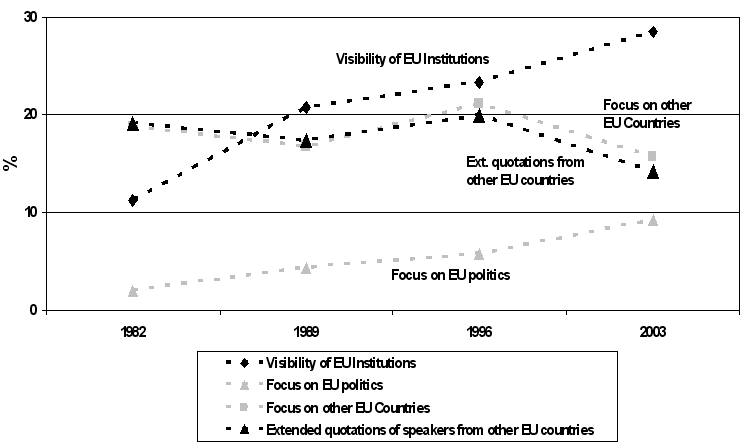
\includegraphics[width=0.95\linewidth]{./SocSci/Wessler.jpg}
%   \mycaption{ xxx )}
    \label{fig:Wessler001}
   \end{center}
\end{figure} \\
Whereas EU institutions and policies are monitored more closely over time in national quality newspapers, and European identity constructions hesitantly enter the public realm in certain instances, the horizontal exchange of opinions between European countries does not increase; national discourse constellations do not become more similar over time. Particular emphasis is placed on case studies of national public debates about Western military interventions, and genetically modified food. Results of Phase I will be published in a number of articles and a monograph with Palgrave Macmillan in 2007. An additional study conducted with IUB students has analyzed online newspapers from ten Eastern and Western European countries with respect to general content characteristics and levels of Europeanization. Apart from work on the European public sphere, Hartmut Wessler has developed a second research line. He completed a pilot study on intercultural aspects of television coverage of the 2003 Iraq war. The project "Different pictures? The Influence of Arab Television Channels on the Image of the Iraq War in Western International Television News Programs" analyzed how Western news channels use material from Arab channels and how they distance themselves from this material at the same time.


\vspace{0.6cm}
\textbf{Funded Projects}\\[-0.25cm]
\begin{enumerate}
\item[$\bullet$]	"The Transnationalization of Public Spheres: The Case of the EU"\newline
funded by the Deutsche Forschungsgemeinschaft as part of the Collaborative Research Center 597 "Transformations of the State"
\end{enumerate}


\vspace{0.6cm}
\textbf{Other Professional Activities}\\[-0.25cm]
\begin{enumerate}
\item[$\bullet$]Deputy member of the board, Collaborative Research Center 597 on "Transformations of the State", funded by the Deutsche Forschungsgemeinschaft
\item[$\bullet$]Reviewer for Volkswagen Foundation, Hannover, \textit{Global Media and Communication, Medien \& Kommunikationswissenschaft, Zeitschrift f�r Medienpsychologie, Journalism: Theory, Practice \& Criticism,} and for Annual conferences of the International Communication Association and the German Communication Association
\end{enumerate}


\vspace{0.6cm}
\textbf{PhD-Students}\\[-0.25cm]

Katharina Kleinen-von K�nigsl�w\newline
\textit{Integration and Segmentation of the National Public Sphere}


\vspace{0.6cm}
\textbf{Research Personnel}\\[-0.25cm]

Michael Br�ggemann\newline
Research Associate in the project "The Transnationalization of Public Spheres: The Case of the EU"\\[-0.15cm]

Stefanie Sifft\newline
Research Associate in the project "The Transnationalization of Public Spheres: The Case of the EU"
\newpage
%Publications for History

%the function for the book publication could be as follows [it was not implemented here]
%1=author;2=year;3=title;4=publisher + comments
%\newcommand{\book}[4]{#1 (#2). \textit{#3}. #4}

\newpage

\subsection{Publications}




	\paragraph{Books} \textit{ }
	
\bigskip	


Dooley, B. (Ed.) (2006). \textit{Energy and culture: Perspectives on the power to work}. Burlington, VT: Ashgate. \\ 

Fischer-Tin\'{e}, H. (2006). \textit{Ausnahmezustand}. Novel by Nirmal Verma, translated from Hindi by H. Fischer-Tin\'{e}, \& H. Bauhaus-L\"{o}tzke. Heidelberg: Draupadi.\\ 

Frey, M. (2006). \textit{Dekolonisierung in S\"{u}dostasien. Die Vereinigten Staaten und die Aufl\"{o}sung der europ\"{a}ischen Kolonialreiche}. M\"{u}nchen: Oldenbourg.\\ 

Leutner, M., Spakowski, N., \& Yu, C.M. (Eds.) (2006). \textit{Gonghe shidai de Zhongguo fun\"{u} (Women in China. The Republican Period in Historical Perspective)}. Taipei: Rive Gauche Publishing, in press.\\ 

Paulmann, J. (2006). \textit{Die Haltung der Zur\"{u}ckhaltung: Ausw\"{a}rtige Selbstdarstellungen nach 1945 und die Suche nach einem erneuerten Selbst-verst\"{a}ndnis in der Bundesrepublik} (= Schriftenreihe der Wilhelm und Helene Kaisen-Stiftung), Bremen: Kaisen-Stiftung.\\ 

Spakowski, N., \& Milwertz, C. (Eds.) (2006). \textit{Women and gender in Chinese Studies. Special issue of Chinese History and Society/Berliner China-Hefte}, 29.\\ 



\paragraph{Articles \& Chapters}\textit{ }

\bigskip


Dooley, B. (2006). Art and information brokerage in the career of Don Giovanni de' Medici. In H. Cools, M. Keblusek, \& B. Noldus (Eds.), \textit{Your Humble Servant} (pp. 81-96). Hilversum: Verloren.\\ 

Fischer-Tin\'{e}, H. (2006). Global civil society and the forces of empire. The Salvation Army, British imperialism and the "pre-history" of NGOs. In S. Conrad, \& D. Sachsenmaier (Eds.), \textit{Conceptions of world order: Global historical approaches} (pp. 25-57). New York: Palgrave, in press.\\ 

Fischer-Tin\'{e}, H. (2006). Stadt der Pal\"{a}ste? - Europ\"{a}ische Lebenswelten im kolonialen Kalkutta. In R. Ahuja, \& C. Brosius (Eds.), \textit{Megast\"{a}dte in Indien: Mumbai, Delhi, Calcutta} (pp. 241-256). Heidelberg: Draupadi. \\ 

Fischer-Tin\'{e}, H. (2006). "Deep Occidentalism"? - Europa und der Westen in der Wahrnehmung hinduistischer Intellektueller und Reformer (ca. 1890-1930). \textit{Journal of Modern European History, 4}(2), 171-203.\\ 

Fischer-Tin\'{e}, H. (2006). From \textit{Brahmacharya} to conscious race culture: Indian nationalism, Hindu tradition and Victorian discourses of science. In C. Bates (Ed.), \textit{Beyond representation. The construction of identity in colonial India }(pp. 230-59). New Delhi: Oxford University Press.\\ 

Fischer-Tin\'{e}, H. (2006). Ananda Marga. In C. Auffahrt, H.-G. Kippenberg, \& A. Michaels (Eds.), \textit{W\"{o}rterbuch der Religionen }(p. 32). Stuttgart: Kr\"{o}ner.\\ 

Fischer-Tin\'{e}, H. (2006). Arya Samaj. In C. Auffahrt, H.-G. Kippenberg, \& A. Michaels (Eds.), \textit{W\"{o}rterbuch der Religionen }(p. 45). Stuttgart: Kr\"{o}ner.\\ 

Fischer-Tin\'{e}, H. (2006). Brahmo Samaj. In C. Auffahrt, H.-G. Kippenberg, \& A. Michaels (Eds.), \textit{W\"{o}rterbuch der Religionen }(p. 80). Stuttgart: Kr\"{o}ner.\\ 

Fischer-Tin\'{e}, H. (2006). Dayanand Sarasvati. In C. Auffahrt, H.-G. Kippenberg, \& A. Michaels (Eds.), \textit{W\"{o}rterbuch der Religionen }(p. 103). Stuttgart: Kr\"{o}ner.\\ 

Fischer-Tin\'{e}, H. (2006). Keshab Chandra Sen. In C. Auffahrt, H.-G. Kippenberg, \& A. Michaels (Eds.), \textit{W\"{o}rterbuch der Religionen} (p. 280). Stuttgart: Kr\"{o}ner.\\ 

Fischer-Tin\'{e}, H. (2006). Krishnamurti. In C. Auffahrt, H.-G. Kippenberg, \& A. Michaels (Eds.), \textit{W\"{o}rterbuch der Religionen} (p. 296). Stuttgart: Kr\"{o}ner.\\ 

Fischer-Tin\'{e}, H. (2006). Maharishi Mahesh Yogi. In C. Auffahrt, H.-G. Kippenberg, \& A. Michaels (Eds.), \textit{W\"{o}rterbuch der Religionen} (p. 318). Stuttgart: Kr\"{o}ner.\\ 

Fischer-Tin\'{e}, H. (2006). Neohinduismus. In C. Auffahrt, H.-G. Kippenberg, \& A. Michaels (Eds.), \textit{W\"{o}rterbuch der Religionen} (pp. 370-371). Stuttgart: Kr\"{o}ner.\\ 

Fischer-Tin\'{e}, H. (2006). Radhakrishnan. In C. Auffahrt, H.-G. Kippenberg, \& A. Michaels (Eds.), \textit{W\"{o}rterbuch der Religionen} (p. 419). Stuttgart: Kr\"{o}ner.\\ 

Fischer-Tin\'{e}, H. (2006). Rajneesh. In C. Auffahrt, H.-G. Kippenberg, \& A. Michaels (Eds.), \textit{W\"{o}rterbuch der Religionen} (p. 419). Stuttgart: Kr\"{o}ner.\\ 

Fischer-Tin\'{e}, H. (2006). Ramana Maharshi. In C. Auffahrt, H.-G. Kippenberg, \& A. Michaels (Eds.), \textit{W\"{o}rterbuch der Religionen} (p. 420). Stuttgart: Kr\"{o}ner.\\ 

Fischer-Tin\'{e}, H. (2006). Sri Aurobindo. In C. Auffahrt, H.-G. Kippenberg, \& A. Michaels (Eds.), \textit{W\"{o}rterbuch der Religionen} (p. 496). Stuttgart: Kr\"{o}ner.\\ 

Fischer-Tin\'{e}, H. (2006). Sundar Singh. In C. Auffahrt, H.-G. Kippenberg, \& A. Michaels (Eds.), \textit{W\"{o}rterbuch der Religionen} (p. 504). Stuttgart: Kr\"{o}ner.\\ 

Fischer-Tin\'{e}, H. (2006). Tagore (Debendranath). In C. Auffahrt, H.-G. Kippenberg, \& A. Michaels (Eds.), \textit{W\"{o}rterbuch der Religionen} (p. 509). Stuttgart: Kr\"{o}ner.\\ 

Fischer-Tin\'{e}, H. (2006). Tagore (Rabindranath). In C. Auffahrt, H.-G. Kippenberg, \& A. Michaels (Eds.), \textit{W\"{o}rterbuch der Religionen} (p. 509). Stuttgart: Kr\"{o}ner.\\ 

Fischer-Tin\'{e}, H. (2006). Vivekananda. In C. Auffahrt, H.-G. Kippenberg, \& A. Michaels (Eds.), \textit{W\"{o}rterbuch der Religionen} (p. 558). Stuttgart: Kr\"{o}ner.\\ 

Frey, M. (2006). Die Vereinigten Staaten und die Dritte Welt w\"{a}hrend des Kalten Krieges. In B. Greiner, \& D. Walther (Eds.), \textit{Hei�e Kriege im Kalten Krieg} (pp. 27-56). Hamburg: Hamburger Edition. \\ 

Frey, M. (2006). Zivilgesellschaft in historischer Perspektive: Die Niederlande und Deutschland im 19. Jahrhundert. \textit{Zentrum f\"{u}r Niederlande-Studien Jahrbuch f\"{u}r 2005, 16}, 11-32.\\ 

Frey, M. (2006). Mao Zedong. Nationalist und Despot. In S. F\"{o}rster, \& M. P\"{o}hlmann (Eds.), \textit{Kriegsherren der Weltgeschichte. 22 Historische Portraits} (pp. 357-372). M\"{u}nchen: C.H. Beck.\\ 

Spakowski, N., \& Milwertz, C. (2006). Introduction: Women and gender in Chinese Studies and the Women and Gender in Chinese Studies Network (WAGNet). In N. Spakowski, \& C. Milwertz (Eds.), \textit{Women and Gender in Chinese Studies}. Special issue of \textit{Chinese History and Society/Berliner China-Hefte, 29}, 3-4.\\ 

Spiekermann, U. (2006). From neighbour to consumer. The transformation of retailer-consumer relationships in twentieth-century Germany. In F. Trentmann (Ed.), \textit{The making of the consumer. Knowledge, power and identity in the modern world} (pp. 147-174). Oxford: Berg.\\ 

Spiekermann, U. (2006). Warum scheitert Ern\"{a}hrungskommunikation? In Aid e.V. (Ed.), \textit{Ern\"{a}hrungskommunikation. Neue Wege - neue Chancen?}. (pp. 11-20). Bonn: Aid.\\ 

Spiekermann, U. (2006). Warum scheitert die Ern\"{a}hrungskommunikation? Eine Antwort aus kulturwissenschaftlicher Perspektive. In E. Barl\"{o}sius, \& R. Rehaag (Ed.), \textit{Anforderungen an eine \"{o}ffentliche Ern\"{a}hrungskommunikation} (pp. 39-51). Berlin: Wissenschaftszentrum.\\ 

Spiekermann, U. (2006). Warenwelten. Die Normierung der Nahrungsmittel in Deutschland 1880-1930. In R.-E. Mohrmann (Ed.), \textit{Essen und Trinken in der Moderne} (pp. 99-124). M\"{u}nster: Waxmann.\\ 

Spiekermann, U. (2006). Brown bread for victory: German and British wholemeal politics in the interwar period. In F. Trentmann, \& F. Just (Ed.), \textit{Food and conflict in Europe in the age of the two World Wars} (pp. 143-171). Basingstoke: Palgrave Macmillan.\\ 

\newpage
%Lecture Talks for ISS

\newpage
\subsection{Invited Scientific Lectures and Talks}


{\hyphenpenalty=7000
\begin{flushleft}
January 2006\\[0.5cm] 
\end{flushleft}
\begin{tabular}{lp{13.4cm}}
 Speaker:	&  Gert Brunekreeft  \\
 Place: 	 & Wiesbaden \\
 Event:   &	Lecture series of the Hessisches Wirtschaftsministerium "Vorrang f\"{u}r Markt und Wettbewerb" \\
 Title: &	 Erfahrungen mit Anreizregulierung \\ \\
\end{tabular}
\begin{tabular}{lp{13.4cm}}
 Speaker:	&  Gert Brunekreeft  \\
 Place: 	 & Vienna, Austria \\
 Event:   &	Conference Wirtschaftsuniversit\"{a}t Wien \\
 Title: &	Regulation and Investment \\ \\
\end{tabular}
\begin{tabular}{lp{13.4cm}}
 Speaker:	&  Christian Joppke  \\
 Place: 	 & The Nixon Center, Washington, D.C., USA \\
 Event:   &	Guest lecture \\
 Title: &	European Immigrant Integration \\ \\
\end{tabular}
\begin{tabular}{lp{13.4cm}}
 Speaker:	&  Wolfgang Pfaffenberger  \\
 Place: 	 & Universit\"{a}t Bremen, FB 4 \\
 Event:   &	Guest lecture \\
 Title: &	Zukunftsprobleme der Stromversorgung \\ \\
\end{tabular}



\begin{flushleft}
February 2006\\[0.5cm]
\end{flushleft}
\begin{tabular}{lp{13.4cm}}
 Speaker:	&  Wolfgang Pfaffenberger  \\
 Place: 	 & Institut f\"{u}r \"{o}konomische Bildung, Oldenburg \\
 Event:   &	Annual conference of \"{o}konomische Bildung Online \\
 Title: &	F\"{u}nf popul\"{a}re Irrt\"{u}mer zum Energiethema dargestellt anhand \"{o}konomischer Para-digmen \\ \\
\end{tabular}
\begin{tabular}{lp{13.4cm}}
 Speaker:	&  Michael Br\"{u}ggemann  \\
 Place: 	 & Z\"{u}rich, Switzerland \\
 Event:   &	DPGuK/DVPW-Fachgruppentagung "Media Governance" \\
 Title: &	Governance durch Kommunikation? Genesis einer europ\"{a}ischen Informationspolitik \\ \\
\end{tabular}



\begin{flushleft}
March 2006\\[0.5cm]
\end{flushleft}
\begin{tabular}{lp{13.4cm}}
 Speaker:	&  Andreas Bausch  \\
 Place: 	 & Giessen \\
 Event:   &	GIUS, Giessener Unternehmungsf\"{u}hrungsseminar \\
 Title: &	Wertorientiertes Management \\ \\
\end{tabular}
\begin{tabular}{lp{13.4cm}}
 Speaker:	&  Hilke Brockmann  \\
 Place: 	 & Princeton University \\
 Event:   &	Conference of the Global Network on Inequality Research as Part of the 75$^{\textrm{th}}$ Anniversary of the Woodrow Wilson School on "New Directions in the Studies of Inequality and Stratification" \\
 Title: &	 Reforms that Go under your Skin. Age, Cohort, and Period Inequalities in Advanced Welfare States \\ \\
\end{tabular}
\begin{tabular}{lp{13.4cm}}
 Speaker:	&  Philipp Genschel  \\
 Place: 	 & London School of Economics, England \\
 Event:   &	Practitioners' Forum on "Policy Learning and Experimentation in EU Economic Governance: Laboratory Federalism in Practice?" \\
 Title: &	Tax Competition, Tax Harmonization and Tax Innovation \\ \\
\end{tabular}
\begin{tabular}{lp{13.4cm}}
 Speaker:	&  Christian Joppke  \\
 Place: 	 & Catholic University of Leuven, Belgium \\
 Event:   &	Guest lecture \\
 Title: &	Toward a Multicultural Europe? A Social Science Perspective \\ \\
\end{tabular}
\begin{tabular}{lp{13.4cm}}
 Speaker:	&  Christian Joppke  \\
 Place: 	 & Institut de Sociologie, Universite Libre de Bruxelles, Belgium \\
 Event:   &	Seminar \\
 Title: &	The Transformation of Immigrant Integration in Western Europe \\ \\
\end{tabular}
\begin{tabular}{lp{13.4cm}}
 Speaker:	&  Wolfgang Pfaffenberger  \\
 Place: 	 & Danish Environmental Assessment Institute, Copenhagen, Denmark \\
 Event:   &	Conference "Green Roads to Growth" \\
 Title: &	 Renewable Energies - Environmental Benefits, Economic Growth and Job Creation\\ \\
\end{tabular}
\begin{tabular}{lp{13.4cm}}
 Speaker:	&   	Wolfgang Pfaffenberger \\
 Place: 	 & Umweltbundesamt Berlin \\
 Event:   &	Kraftwerksforum \\
 Title: &	Kraftwerke in Deutschland, Stand und Ausblick \\ \\
\end{tabular}
\begin{tabular}{lp{13.4cm}}
 Speaker:	&  Wolfgang Pfaffenberger  \\
 Place: 	 & Oldenburg \\
 Event:   &	Innovationsforum "Zuk\"{u}nftige Energieversorgung" \\
 Title: &	Neue Herausforderungen in der Energiewirtschaft - regionales Beispiel W\"{a}rmemarkt \\ \\
\end{tabular}
\begin{tabular}{lp{13.4cm}}
 Speaker:	&  Welf Werner  \\
 Place: 	 & Bonn \\
 Event:   &	Jahrestagung Verein f\"{u}r Socialpolitik \\
 Title: &	Zur Entwicklung der Sozialpolitik in der Bundesrepublik Deutschland seit dem Zweiten Weltkrieg: Eine europ\"{a}ische Perspektive \\ \\
\end{tabular}
\begin{tabular}{lp{13.4cm}}
 Speaker:	&  Welf Werner  \\
 Place: 	 & Atlantische Akademie Rheinland-Pfalz, Boppard \\
 Event:   &	Workshop "Germany and the United States: Separated by Common Values"? \\
 Title: &	Values in U.S. and German Labor Markets \\ \\
\end{tabular}


\newpage
\begin{flushleft}
April 2006\\[0.5cm] 
\end{flushleft}
\begin{tabular}{lp{13.4cm}}
 Speaker:	&  Christian Joppke  \\
 Place: 	 & Vrije Universiteit Amsterdam, Netherlands \\
 Event:   &	Seminar \\
 Title: &	State Neutrality and Anti-Veiling Laws in France and Germany \\ \\
\end{tabular}
\begin{tabular}{lp{13.4cm}}
 Speaker:	&  Hon Hei Bob Tsang  \\
 Place: 	 & \"{U}berseemuseum Bremen \\
 Event:   &	Lecture series "Chinesische Kultur zwischen Tradition und Moderne" \\
 Title: &	Kungfu-Filme als Ausdruck chinesischer Identit\"{a}t? \\ \\
\end{tabular}
\begin{tabular}{lp{13.4cm}}
 Speaker:	&  Hartmut Wessler  \\
 Place: 	 & University of Z\"{u}rich, Institute Mass Communication and Media Research, Switzerland \\
 Event:   &	Lecture Series \\
 Title: &	Transnationalization und Europeanization of the Political Public Sphere\\ \\
\end{tabular}



\begin{flushleft}
May 2006\\[0.5cm]
\end{flushleft}
\begin{tabular}{lp{13.4cm}}
 Speaker:	&  Philipp Genschel  \\
 Place: 	 & Centre Cournot Paris, France \\
 Event:   &	Public Debate on "Fiscal Harmonization in the EU" \\
 Title: &	Tax Competition, Tax Harmonization and Subsidiarity in the EU \\ \\
\end{tabular}
\begin{tabular}{lp{13.4cm}}
 Speaker:	&   Wolfgang Pfaffenberger \\
 Place: 	 & Brazil \\
 Event:   &	Uni\~{a}o Europeia e America Latina: Caminhos para uma nova Agenda, Brasilia \\
 Title: &	Energy and Natural Resources \\ \\
\end{tabular}
\begin{tabular}{lp{13.4cm}}
 Speaker:	&  Christian Welzel  \\
 Place: 	 & Department of Political Science, University of California, Berkeley, USA \\
 Event:   &	Guest lecture \\
 Title: &	The Human Development Model of Social Change \\ \\
\end{tabular}
\begin{tabular}{lp{13.4cm}}
 Speaker:	&  Christian Welzel  \\
 Place: 	 & Center for the Study of Democracy, University of California, Irvine, USA \\
 Event:   &	Guest lecture \\
 Title: &	The Human Development Model of Social Change \\ \\
\end{tabular}
\begin{tabular}{lp{13.4cm}}
 Speaker:	&  Welf Werner  \\
 Place: 	 & Institut Historique Allemand, Paris, France \\
 Event:   &	Conference "Atelier historique franco-allemand sur les relations economiques et financieres" \\
 Title: &	La cooperation entre compagnies fran�aises et allemandes dans les marches de la reassurance transatlantique durant le second XXe siecle \\ \\
\end{tabular}
\begin{tabular}{lp{13.4cm}}
 Speaker:	& Hartmut Wessler   \\
 Place: 	 & Ludwig-Boltzmann-Institute for European History and Public Spheres, Vienna, Austria \\
 Event:   &	Boltzmann History Roundtable 1 "Transnational Historiography, European Public Spheres" \\
 Title: &	Conceptions of Europe's Public Sphere \\ \\
\end{tabular}


\begin{flushleft}
June 2006\\[0.5cm] 
\end{flushleft}
\begin{tabular}{lp{13.4cm}}
 Speaker:	&  Philipp Genschel  \\
 Place: 	 & Universit\"{a}t Bielefeld \\
 Event:   &	Conference on "Mutual Recognition as a New Mode of Governance" \\
 Title: &	Mutual Recognition in Regulation and Taxation \\ \\
\end{tabular}
\begin{tabular}{lp{13.4cm}}
 Speaker:	&  Marion G. M\"{u}ller  \\
 Place: 	 & Dresden \\
 Event:   &	56$^{\textrm{th}}$ Annual Conference of the International Communication Association (ICA) \\
 Title: &	The Image is the Message: A Model for Applying Iconology in Mass Media Research \\ \\
\end{tabular}
\begin{tabular}{lp{13.4cm}}
 Speaker:	&  Ayse Esra \"{O}zcan  \\
 Place: 	 & Dresden \\
 Event:   &	56$^{\textrm{th}}$ Annual Conference of the International Communication Association (ICA) \\
 Title: &	Visual Representation of the Female in the Turkish Press \\ \\
\end{tabular}
\begin{tabular}{lp{13.4cm}}
 Speaker:	&  Welf Werner  \\
 Place: 	 & Schlo� Reichertshausen, European Business School \\
 Event:   &	Guest lecture \\
 Title: &	Good Governance in Times of Globalization; Globalization Now and Then: Lessons from Two Centuries of Economic Integration and Disintegration \\ \\
\end{tabular}



\begin{flushleft}
July 2006\\[0.5cm] 
\end{flushleft}
\begin{tabular}{lp{13.4cm}}
 Speaker:	&  Andreas Bausch  \\
 Place: 	 & Scoul, Switzerland \\
 Event:   &	Summer Event of The Advisory House AG \\
 Title: &	Unternehmenswachstum und Performance - Evidence-Based Best Practices \\ \\
\end{tabular}
\begin{tabular}{lp{13.4cm}}
 Speaker:	&  Andreas Bausch  \\
 Place: 	 & Friedrich-Schiller-Universit\"{a}t Jena \\
 Event:   &	Guest Lecture \\
 Title: &	 Normatives und strategisches Management in internationalen Unternehmen\\ \\
\end{tabular}
\begin{tabular}{lp{13.4cm}}
 Speaker:	&  Andreas Bausch  \\
 Place: 	 & Friedrich-Schiller-Universit\"{a}t Jena \\
 Event:   &	Seminar \\
 Title: &	International Mergers, Acquisitions and Alliances \\ \\
\end{tabular}
\begin{tabular}{lp{13.4cm}}
 Speaker:	&  Matthijs Bogaards  \\
 Place: 	 & Fukuoka, Japan \\
 Event:   &	20$^{\textrm{th}}$ World Congress of International Political Science Association \\
 Title: &	Measuring Democracy through Election Outcomes: A Critique with African Data \\ \\
\end{tabular}
\begin{tabular}{lp{13.4cm}}
 Speaker:	&  Philipp Genschel  \\
 Place: 	 & Max-Planck-Institute for the Study of Societies \\
 Event:   &	Conference on "Die Europ\"{a}ische Union: Governance und Policy-Making" \\
 Title: &	F\"{u}hrt die Europ\"{a}ische Integration zu "falschem Bewu�tsein?" \\ \\
\end{tabular}
\begin{tabular}{lp{13.4cm}}
 Speaker:	&  Philipp Genschel  \\
 Place: 	 & Universit\"{a}t Trier \\
 Event:   &	 Annual Meeting of the Society for the Advancement of Socio-Economics\\
 Title: &	Tax Competition as a Dependent Variable (with Thomas Rixen) \\ \\
\end{tabular}
\begin{tabular}{lp{13.4cm}}
 Speaker:	&  Marion G. M\"{u}ller  \\
 Place: 	 & Wroxton College, England \\
 Event:   &	7$^{\textrm{th}}$ ECPR Workshop of Parliamentary Scholars and Parliamentarians \\
 Title: &	Communicating Parliaments. A Comparative Study of Five Western Parliaments and their Communicative Structures and Functions \\ \\
\end{tabular}
\begin{tabular}{lp{13.4cm}}
 Speaker:	&  Wolfgang Pfaffenberger  \\
 Place: 	 & International Institute of Management Technology, University Fribourg, Switzerland \\
 Event:   &	Guest lecture \\
 Title: &	Zukunft der Stromerzeugung im liberalisierten Markt \\ \\
\end{tabular}
\begin{tabular}{lp{13.4cm}}
 Speaker:	& Stefanie Sifft   \\
 Place: 	 & Fukuoka, Japan \\
 Event:   &	20$^{\textrm{th}}$ World Congress of International Political Science Association \\
 Title: &	Together We Fight? The Legitimacy of Military Interventions and the Europeanization of Public Spheres \\ \\
\end{tabular}
\begin{tabular}{lp{13.4cm}}
 Speaker:	&  Jens Steffek  \\
 Place: 	 & The Hague, Netherlands \\
 Event:   &	CISS Millennium Conference \\
 Title: &	 How much Consensus Does the World Need?\\ \\
\end{tabular}
\begin{tabular}{lp{13.4cm}}
 Speaker:	&  Christian Welzel  \\
 Place: 	 & 	Messezentrum, N\"{u}rnberg \\
 Event:   &	GfK-Jahrestagung \\
 Title: &	Wertewandel in der westlichen Welt \\ \\
\end{tabular}
\begin{tabular}{lp{13.4cm}}
 Speaker:	&  Welf Werner  \\
 Place: 	 & Bremen \\
 Event:   &	Symposium: Bremen und Nordamerika (Carl Schurz Gesellschaft, Bremen United States Center, Universit\"{a}t Bremen) \\
 Title: &	 Auswanderung von Bremen und Bremerhaven in die Neue Welt: Wirtschaftliche Effekte und Bestimmungsgr\"{u}nde\\ \\
\end{tabular}
\begin{tabular}{lp{13.4cm}}
 Speaker:	&  Hartmut Wessler  \\
 Place: 	 & Fukuoka, Japan \\
 Event:   &	20$^{\textrm{th}}$ World Congress of International Political Science Association \\
 Title: &	Different Pictures? The Influence of Arab Televison Channels on the Image of the Iraq War in Western International Television News Programs \\ \\
\end{tabular}


\newpage
\begin{flushleft}
August 2006\\[0.5cm] 
\end{flushleft}
\begin{tabular}{lp{13.4cm}}
 Speaker:	&  Christian Welzel  \\
 Place: 	 & Social Science Faculty, Oslo University, Norway \\
 Event:   &	Oslo Summer School in Social Sciences \\
 Title: &	Democratic Attitudes, Democratic Culture, Democratic Systems \\ \\
\end{tabular}




\begin{flushleft}
September 2006\\[0.5cm] 
\end{flushleft}
\begin{tabular}{lp{13.4cm}}
 Speaker:	&  Philipp Genschel  \\
 Place: 	 & Universit\"{a}t Leipzig \\
 Event:   &	Workshop "Observing globalization" \\
 Title: &	Ambiguities of Tax Competition \\ \\
\end{tabular}
\begin{tabular}{lp{13.4cm}}
 Speaker:	&  Philipp Genschel  \\
 Place: 	 & Universit\"{a}t M\"{u}nster \\
 Event:   &	Triannual Meeting of the German Political Science Association \\
 Title: &	The Institutional Foundations of Tax Competition (with Thomas Rixen) \\ \\
\end{tabular}
\begin{tabular}{lp{13.4cm}}
 Speaker:	&  Wolfgang Pfaffenberger  \\
 Place: 	 & Umweltministerium Baden-W\"{u}rttemberg \\
 Event:   &	Umwelttag 2006 \\
 Title: &	Anforderungen an den Energietr\"{a}germix der Zukunft \\ \\
\end{tabular}
\begin{tabular}{lp{13.4cm}}
 Speaker:	& Jens Steffek   \\
 Place: 	 & Universit\"{a}t M\"{u}nster \\
 Event:   &	23$^{\textrm{rd}}$ Scientific Congress of the Deutsche Vereinigung f\"{u}r Politische Wissenschaft \\
 Title: &	Die Legitimation internationalen Regierens: vom Staatenkonsens zum B\"{u}rgerkonsens? \\ \\
\end{tabular}



\begin{flushleft}
October 2006\\[0.5cm] 
\end{flushleft}
\begin{tabular}{lp{13.4cm}}
 Speaker:	&  Matthijs Bogaards  \\
 Place: 	 & The Clingendael Institute, The Hague, Netherlands \\
 Event:   &	Workshop on Political Party Regulation in Conflict Prone-Societies \\
 Title: &	Ethnic Conflict Management and Parties \\ \\
\end{tabular}
\begin{tabular}{lp{13.4cm}}
 Speaker:	&  Hilke Brockmann  \\
 Place: 	 & Universit\"{a}t Kassel \\
 Event:   &	33$^{\textrm{rd}}$ Congress of the Deutsche Gesellschaft f\"{u}r Soziologie \\
 Title: &	Families and Health \\ \\
\end{tabular}
\begin{tabular}{lp{13.4cm}}
 Speaker:	& Peter Ludes   \\
 Place: 	 & Bremen \\
 Event:   &	Meeting of the Fulbright Group Bremen \\
 Title: &	Teaching and Research at the SHSS of IUB \\ \\
\end{tabular}
\begin{tabular}{lp{13.4cm}}
 Speaker:	&  Wolfgang Pfaffenberger  \\
 Place: 	 & Universit\"{a}t Oldenburg \\
 Event:   &	Opening Session of Graduate Course Renewable Energy \\
 Title: &	 The Role of Renewable Energy in the Future\\ \\
\end{tabular}
\begin{tabular}{lp{13.4cm}}
 Speaker:	&  Wolfgang Pfaffenberger  \\
 Place: 	 & China University of Petroleum, Qindao, China \\
 Event:   &	Guest lecture \\
 Title: &	European Policy for Energy \\ \\
\end{tabular}
\begin{tabular}{lp{13.4cm}}
 Speaker:	&  Wolfgang Pfaffenberger  \\
 Place: 	 & Faculty of Natural Resources, Anhui Normal University, Wuhu, China \\
 Event:   &	Guest lecture \\
 Title: &	European Policy for Energy, Natural Resources and the Environment \\ \\
\end{tabular}
\begin{tabular}{lp{13.4cm}}
 Speaker:	&  Welf Werner  \\
 Place: 	 & Z\"{u}rich, Switzerland \\
 Event:   &	Scientific symposium "Internationalisierung und Globalisierung der Versicherungs-wirtschaft" \\
 Title: &	Volatility of International Reinsurance Markets: An Analysis of US Balance of Payments Statistics\\ \\
\end{tabular}


\begin{flushleft}
November 2006\\[0.5cm]
\end{flushleft}
\begin{tabular}{lp{13.4cm}}
 Speaker:	&  Matthijs Bogaards  \\
 Place: 	 & Balstahl, Switzerland \\
 Event:   &	Annual Meeting of the Swiss Political Science Conference \\
 Title: &	 From Degree to Type: The Difficult Art of Drawing the Line in Continuous Measures of Democracy\\ \\
\end{tabular}
\begin{tabular}{lp{13.4cm}}
 Speaker:	&  Gert Brunekreeft  \\
 Place: 	 & Bergisch-Gladbach \\
 Event:   &	2. Bonner Energiegespr\"{a}ch \\
 Title: &	Regulierung und Netzinvestitionen \\ \\
\end{tabular}
\begin{tabular}{lp{13.4cm}}
 Speaker:	&  Gert Brunekreeft  \\
 Place: 	 & London, England  \\
 Event:   &	Workshop "Liberalisation of Air Transport, Airport Regulation and Benchmarking" \\
 Title: &	On Regulation and Benchmarking of Energy Networks \\ \\
\end{tabular}
\begin{tabular}{lp{13.4cm}}
 Speaker:	&  Franziska Deutsch  \\
 Place: 	 & Glocke, Bremen \\
 Event:   &	Sichtweisen \\
 Title: &	S\"{u}�es Ja und bitteres Nein (together with Amina \"{O}zelsel) \\ \\
\end{tabular}
\begin{tabular}{lp{13.4cm}}
 Speaker:	&  Peter Ludes  \\
 Place: 	 & Antalya, Turkey \\
 Event:   &	Mass Media and Communications Research Network Meeting of the European Sociological Association\\
 Title: &	 Key Visual Networks \\ \\
\end{tabular}
\begin{tabular}{lp{13.4cm}}
 Speaker:	&  Peter Ludes  \\
 Place: 	 & Bremen \\
 Event:   &	MEP Baltic Teachers' Seminar \\
 Title: &	Visual Networks: Brazil, China, Germany, and the United States \\ \\
\end{tabular}
\begin{tabular}{lp{13.4cm}}
 Speaker:	& Wolfgang Pfaffenberger   \\
 Place: 	 & Groningen, Netherlands \\
 Event:   &	Energy Convention Groningen 2006 \\
 Title: &	Energy Transition in Germany \\ \\
\end{tabular}
\begin{tabular}{lp{13.4cm}}
 Speaker:	&  Christian Welzel  \\
 Place: 	 & Bogacizi University, Istanbul, Turkey \\
 Event:   &	World Values Surveys Association \\
 Title: &	A Human Development Model of Global Cultural Change \\ \\
\end{tabular}
\begin{tabular}{lp{13.4cm}}
 Speaker:	&  Hartmut Wessler  \\
 Place: 	 & Austrian Academy of Sciences, Vienna, Austria \\
 Event:   &	Workshop "Comparative Media and Communication Research" \\
 Title: &	Comparing Mediated Public Spheres \\ \\
\end{tabular}


\begin{flushleft}
December 2006\\[0.5cm]
\end{flushleft}
\begin{tabular}{lp{13.4cm}}
 Speaker:	&  Andreas Bausch  \\
 Place: 	 & Bremen \\
 Event:   &	Meeting Lion's Club Bremen \\
 Title: &	Strategische Erfolgsfaktoren von Unternehmen: Ergebnisse evidenzbasierter Strategieforschung \\ \\
\end{tabular}
\begin{tabular}{lp{13.4cm}}
 Speaker:	& Philipp Genschel   \\
 Place: 	 & Friedrich-Ebert-Foundation, Berlin \\
 Event:   &	Conference on "Harmonisierung - Kooperation - Wettbewerb. Steuerpolitische Vorschl\"{a}ge in und f\"{u}r Europa" \\
 Title: &	Harmonisierung forcieren? \\ \\
\end{tabular}
\begin{tabular}{lp{13.4cm}}
 Speaker:	&  Christian Welzel  \\
 Place: 	 & Printmedia Academy, Heidelberg \\
 Event:   &	Print Media Dialog 2006 \\
 Title: &	Wertewandel in der westlichen Welt: Triebkr\"{a}fte und Folgen \\ \\
\end{tabular}
\begin{tabular}{lp{13.4cm}}
 Speaker:	&  Hartmut Wessler  \\
 Place: 	 & Luzern, Switzerland \\
 Event:   &	Mediensymposium Luzern 2006 "Seismographische Funktion von \"{o}ffentlicher Kommunikation im Wandel" \\
 Title: &	Mediale Zungangsschleusen. Die Repr\"{a}sentanz politischer und gesellschaftlicher Akteure in der Medienarena im internationalen und Langzeit-Vergleich \\ 
\end{tabular}

}

\newpage
\section{Statistics and Methods}
\shorttitle{Statistics and Methods}
\subsection{Prof. Dr. Klaus Boehnke}

\textbf{Main Research Interests}\\[-0.25cm]
\begin{enumerate}
\item[$\bullet$]	Political Socialization
\item[$\bullet$]	Value Transmission
\item[$\bullet$]	Social Science Methodology
\item[$\bullet$]	Educational Sociology
\end{enumerate}

\vspace{0.5cm}
\textbf{Research Activities}\\[-0.25cm]

As in prior years, research of Klaus Boehnke focused primarily on processes of political socialization among youth and young adults, often employing a cross-cultural perspective. Two major research projects have been conducted. The first project studied effects of the EU Eastern enlargement on the mobilization of right-wing extremism in Germany and bordering regions in Poland and the Czech Republic, with funding from the Deutsche Forschungsgemeinschaft. This study encompassed representative samples of the border regions of the three countries and is a longitudinal continuation of a study previously funded by the Federal Ministry of Education and Science (BMBF). The second project was a long-term panel study of young peace-movement sympathizers from the mid 1980s who have been studied every 3 � years since 1985. In 2006 the seven panel wave was conducted. That study focuses on the impact of societal context on individual psychosocial well-being and political activism. In the report phase, work has also continued on two other research projects, one on value transmission in families, another one on problems of social exclusion as a consequence of high achievement in schools ("Streber" study). In addition Klaus Boehnke has prepared two research proposals, one to the BMBF together with Professor Ariel Knafo from the Hebrew University of Jerusalem on identity development and value transmission among migrant youth, and the other to the Deutsche Forschungsgemeinschaft together with Professor Petra Lietz and Dr. Nongkran Wongsri from Saint Louis College in Thailand on learning styles of native and sojourner students in Germany and Thailand. He also prepared a proposal to the Deutsche Forschungsgemeinschaft together with Professor Ulrich K�hnen to obtain funding for the 19$^{\textrm{th}}$ International Congress of Cross-Cultural Psychology, which he hosts together with Ulrich K�hnen at IUB in 2008.

\vspace{0.5cm}
\textbf{Funded Projects}\\[-0.25cm]
\begin{enumerate}
\item[$\bullet$]	"Social integration after the fourth round of EU enlargement-border 	regions as test cases for Europe's path to a transnational civil society",	funded by the Deutsche Forschungsgemeinschaft
\end{enumerate}

\vspace{0.5cm}
\textbf{Organization of Scientific Conferences}\\[-0.25cm]
\begin{enumerate}
\item[$\bullet$]	June 2006\\
Multiliteracy and the European Educational Agenda, 1st international LANGSCAPE conference in conjunction with 3rd Bremen Conference on Content and Language Integrated Learning\\
(organized together with Professor Gerhard Bach from Universit�t Bremen)\\
funded by the Deutsche Forschungsgemeinschaft\\
international participants: 45\\[-0.15cm]

\item[$\bullet$]	July 2006\\
19th Biennial Meeting of the International Society for Behavioral Development\\
Melbourne, Australia\\
Member of the Review Panel\\
international participants: approx. 600\\[-0.15cm]

\item[$\bullet$]	July 2006\\
18th International Congress of Cross-Cultural Psychology\\
Spetses, Greece\\
Member of the International Scientific Program Committee\\
international participants: approx. 600\\[-0.15cm]

\item[$\bullet$]	July 2006\\
28th International Congress of Applied Psychology\\
Athens, Greece\\
Program Chair for the Political Psychology Program\\
international participants: approx. 1.800\\[-0.15cm]

\item[$\bullet$]	September 2006\\
45. Kongress der Deutschen Gesellschaft f�r Psychologie\\
N�rnberg\\
Senior Reviewer for Political Psychology
\end{enumerate}

\vspace{0.5cm}
\textbf{Other Professional Activities}\\[-0.25cm]
\begin{enumerate}
\item[$\bullet$]	College Master of Mercator College at the International University Bremen
\item[$\bullet$]	Secretary-General of the International Association for Cross-Cultural Psychology
\item[$\bullet$]	President of the Division of Political Psychology of the International Association for Applied Psychology
\item[$\bullet$]	President of the German Peace Psychology Association (\textit{Forum Friedenspsychologie})
\item[$\bullet$]	Member of the Executive Board of the Youth Sociology Section of the German Sociological Association (DGS)
\item[$\bullet$]	Ad hoc Expert Evaluator for the Deutsche Forschungsgemeinschaft
\item[$\bullet$]	Expert Evaluator for the European Commission in the 6th Framework Program, NEST, and the Marie Curie Program
\item[$\bullet$]	Expert Evaluator for INTAS
\item[$\bullet$]	Expert Evaluator for the Austrian National Science Foundation
\item[$\bullet$]	Expert Evaluator for the Israel Science Foundation
\item[$\bullet$]	Expert Evaluator for the Economic and Social Science Research Council, United Kingdom
\item[$\bullet$]	Consulting Editor of Peace and Conflict: The Journal of Peace Psychology
\item[$\bullet$]	Consulting Editor of the Journal of Cross-Cultural Psychology
\item[$\bullet$]	Member of the Editorial Board of the International Journal of Behavioral Development
\item[$\bullet$]	Member of the Editorial Board of \textit{Conflict \& Communication online}
\item[$\bullet$]	Senior Advisor of the Committee for Psychological Study of Peace (CPSP) of the International Union of Psychological Science (lUPsyS)
\item[$\bullet$]	Official Liaison (Vertrauensdozent) of Heinrich-B�ll-Stiftung at IUB
\item[$\bullet$]	Ad hoc reviewer for \textit{European Journal of Personality, European Journal for Psychology of Education, European Journal of Social Psychology, European Psychologist, European Societies, International Journal of Behavioral Development, International Journal of Psychology, Journal of Behavioral Science, Journal of Cross-Cultural Psychology, Journal of Public Health, Journal of Social and Clinical Psychology, Peace and Conflict: The Journal of Peace Psychology, Political Psychology, Politische Vierteljahresschrift, Social Psychology of Education: An International Journal, Zeitschrift f�r Medienpsychologie}
\item[$\bullet$]	IUB-Coordinator of the application for a Bremen International Graduate School of Social Sciences ($^{\rm\bf BI}${\itshape GSSS}) in the framework of the Excellence Initiative
\item[$\bullet$]	IUB-Fachkoordinator for the evaluation of sociology in Germany, conducted by the Wissenschaftsrat
\item[$\bullet$]	Member of the Promotion Committee of the Jacobs Center for Lifelong Learning and Institutional Development
\end{enumerate}

\vspace{0.5cm}
\textbf{PhD-Students}\\[-0.25cm]

Daniel Fuss\newline
\textit{Europa als Quelle sozialer Identit\"at--Eine international vergleichende\newline Analyse ihrer Voraussetzungen und Wirkungen bei jungen Erwachsenen}\newline
Defense: December 2006 \\[-0.15cm]

Simone Heil\newline
Working title: \textit{German-Israeli Youth Exchange Programs}\\[-0.15cm]

Angela Kindervater\newline
\textit{Stereotype versus Vorurteile: Welche Rolle spielt Autoritarismus? Ein empirischer Beitrag zur Begriffsbestimmung}\newline
Defense: September 2006\\[-0.15cm]

Olena Kornyeyeva\newline
Working title: \textit{Immigrant Adaptations and Modes of Upbringing}\\[-0.15cm]

Gukaah Brenda Nwana\newline
Working title: \textit{African Immigrants in Germany}\\[-0.15cm]

Martina Schreiber\newline
Working title: \textit{Football Hooliganism in a Social Psychological Perspective}


\vspace{0.6cm}
\textbf{Research Personnel}\\[-0.25cm]

Daniel Fuss\newline
Research Associate\newline
funded by Deutsche Forschungsgemeinschaft

\vspace{0.6cm}
\textbf{Guests}\\[-0.25cm]

Dr. Nongkran Wongsri\newline
Dean of the Faculty of Liberal Arts, Saint Louis College Bangkok, funded by the Deutsche Forschungsgemeinschaft (3 weeks)
\newpage
\subsection{Prof. Dr. Petra Lietz}

\textbf{Main Research Interests}\\[-0.25cm]
\begin{enumerate}
\item[$\bullet$]	Internationally Comparative Research in Education
\item[$\bullet$]	Multivariate and Multilevel Path Models
\end{enumerate}

\vspace{0.6cm}
\textbf{Research Activities}\\[-0.25cm]

Petra Lietz's main research activity in 2006 was the conduct of the second qualitative phase and the third quantitative phase of my research project entitled "Values and learning approaches of IUB's class of 2007". This project is aimed at: (a) examining the way in which different factors operate to influence the achievement of sojourner students, (b) verifying and expanding the understanding of three types of learning approaches, namely achieving, deep and surface learning, and (c) measuring changes in values and learning approaches over time. Analyses of a first path model suggest that personal values can be meaningfully linked to learning approaches and that differences in terms of values exist across genders and across the natural and social sciences. Petra Lietz was also involved in the preparation of two research proposals to the Deutsche Forschungsgemeinschaft, one within the framework of the Forschergruppe "\textit{Priorisierung in der Medizin}", coordinated by Professor Adele Diederich (see Chapter 7 of this report), the other with Professor Klaus Boehnke and Dr. Nongkran Wongsri from Saint Louis College in Bangkok on learning styles of native and sojourner students in a German-Thai comparison.


\vspace{0.6cm}
\textbf{Other Professional Activities}\\[-0.25cm]
\begin{enumerate}
\item[$\bullet$]	Research consultancy for the International Association for the Evaluation of Educational Achievement (IEA) to assist the countries involved with the analyses for and writing of the publication \textit{Arabic Report on the Third International Mathematics and Science Study 2003 database}.
\item[$\bullet$]	Cultures, Markets and Citizens Research Group - CMC
\item[$\bullet$]	Center for International Studies at IUB - CIS
\item[$\bullet$]	Business and Professional Women in Bremen (BPW)
\item[$\bullet$]	Reviewer for \textit{International Education Journal}, Higher Education Research and Development (HERD), Mathematics Education Journal, Zeitschrift f�r Medienpsychologie
\end{enumerate}

\vspace{0.6cm}
\textbf{PhD-Students}\\[-0.25cm]

Katrin Viertel\newline
\textit{Family Affairs: Reception and Effects of TV's Representation of Everyday Family Life}
\newpage
\subsection{Prof. Dr. Margrit Schreier}


\textbf{Main Research Interests}\\[-0.25cm]
\begin{enumerate}
\item[$\bullet$]	Qualitative Research Methods
\item[$\bullet$]	Media Psychology
\item[$\bullet$]	Gender and Reading
\item[$\bullet$]	Persuasive Effects of Fiction
\end{enumerate}

\vspace{0.6cm}
\textbf{Research Activities}\\[-0.25cm]

In 2006, Margrit Schreier has in the first place continued her work on the persuasive effects of fiction, with a special emphasis on degree of involvement as a moderator variable. A second focus has been on gender differences in the experience of reading fiction (funding for this research is provided by the DFG). The results of a first study are in line with previous research to the extent that women prefer to read in order to be drawn into a different world and in order to escape from everyday problems, whereas men are more likely to read for information. Even stronger differences in reading preferences and styles are obtained, however, for the comparison not of men and women, but of gender-schematic and a-schematic persons. A-schematic persons combine the reading interests usually ascribed to either men or women: they are more interested in reading in general, especially in reading nonfiction, and at the same time they read primarily in order to identify with the characters in the fictional world. Another study testing the effects of genre and substantive focus of a fictional narrative on degree of involvement, with both self-report and physiological measures of involvement taken into account, is in the process of being analyzed. A third focus has been on qualitative research methods and methodology, especially on content analysis and strategies of purposive sampling, resulting in a number of publications.


\vspace{0.6cm}
\textbf{Funded Projects}\\[-0.25cm]

"Gender and reading: the effect of text and reader characteristics on the experience of reading fiction" (Lesen und Geschlecht: Differentielles Lese-Erleben in Abh�ngigkeit von Text- und Personenmerkmalen), funded by the Deutsche Forschungsgemeinschaft.


\vspace{0.6cm}
\textbf{Other Professional Activities}\\[-0.25cm]
\begin{enumerate}
\item[$\bullet$]	Since January 2005: Editor-in-chief of the "Zeitschrift f�r Medienpsychologie"
\item[$\bullet$]	Membership in the Editorial Review Boards of the following journals: \textit{Forum Qualitative Social Research, Human Communication Research, Media Psychology, Poetics}
\item[$\bullet$]	Reviewer for the above journals and for DFG grant proposals
\item[$\bullet$]	Workshops on "Qualitative Content Analysis" at ZUMA
\item[$\bullet$]	Teaching cooperation on qualitative methods with the GSSS (Graduate School of Social Sciences, Bremen University)
\item[$\bullet$]	Member of the Advisory Board of INQUA (Institut f�r Qualitative Forschung, Berlin)
\end{enumerate}


\vspace{0.6cm}
\textbf{PhD-Students}\\[-0.25cm]

�zen Oda$\breve{\textrm{g}}$\newline
\textit{Unterschiede und Gemeinsamkeiten zwischen Frauen und M�nnern beim Lesen von Erz�hltexten - eine empirische Studie}\\[-0.15cm]

Yvonne Thies-Brandner\newline
\textit{Safer Sex through Entertainment Education? Realizing the Entertainment Education Approach with Computer Games about HIV/AIDS}\\[-0.15cm]

Bob Tsang\newline
\textit{The Hong Kong Museum of History: its Role in the Construction of Chinese Identity in Pre- and Post-1997 Hong Kong}
\newpage
\subsection[Dr. Michael A. Talias] {Dr. Michael A. Talias{\normalfont\normalsize\newline (Lecturer in Statistics)}}

\vspace{0.3cm}
\textbf{Main Research Interests}\\[-0.25cm]
\begin{enumerate}
\item[$\bullet$]	Applied Multivariate Data Analysis
\item[$\bullet$]	Bandit Problem
\item[$\bullet$]	Sequential Analysis and Optimal Stopping
\item[$\bullet$]	Statistical Decision Theory
\end{enumerate}


\vspace{0.6cm}
\textbf{Research Activities}\\[-0.25 cm]

Michael Talias' research is concerned with the use of sequential statistical methodologies and their relation to the Portfolio management in the Pharmaceutical Industry with the Bayesian Decision framework. Other activities are related to applications of sequential analysis to mathematical finance problems and statistical data analysis in marketing. Michael Talias has also elaborated problems of information theory in the framework of teaching a University Studies Course in the fall semester of 2006.
\newpage
\subsection{Prof. Dr. Adalbert F.X. Wilhelm}


\textbf{Main Research Interests}\\[-0.25cm]
\begin{enumerate}
\item[$\bullet$]	Exploratory Data Analysis and Statistical Modeling
\item[$\bullet$]	Interactive Statistical Graphics
\item[$\bullet$]	Information Visualization and Visual Data Mining
\item[$\bullet$]	Knowledge Management in Web-based Communities
\item[$\bullet$]	Computational Statistics
\end{enumerate}

\vspace{0.6cm}
\textbf{Research Activities}\\[-0.25cm]

As in previous years, Adalbert Wilhelm focused in his research on exploratory approaches to data analysis and modeling. The collaboration within the Key Visuals Project has been continued and some initial data exploration has been performed to detect structures in the semantic information of video material that has been annotated by mass communication scholars. Data Mining procedures like association rules and classification trees have been adapted to investigate relationships and rules within the semantic information. Some heuristics have been developed to devise representative samples of web pages and annual reviews in this context. The behavior of various cluster analysis techniques has been studied and a new complex cluster scheme has been devised which is currently in the implementation phase. Based on prior research in the area of knowledge management the focus has been shifted on incorporating the aspect of innovation into the framework of online-knowledge communities. The major research question is, how innovation processes can be optimally supported in the cooperative context of private-public Communities of Practice. Within this framework, the research focuses on the factors that influence, support, and stimulate innovation processes - as measured by the three constructs (knowledge transfer, knowledge communication and knowledge creation).


\vspace{0.6cm}
\textbf{Other Professional Activities}\\[-0.25cm]
\begin{enumerate}
\item[$\bullet$]	Reviewer for SFI, Science Foundation Ireland
\item[$\bullet$]	Associate Editor \textit{Computational Statistics and Data Analysis}
\item[$\bullet$]	Associate Editor \textit{Computational Statistics}
\item[$\bullet$]	Associate Editor \textit{Journal of Computational and Graphical Statistics}
\item[$\bullet$]	Vertrauensdozent der \textit{Stiftung der Deutschen Wirtschaft}
\end{enumerate}


\vspace{0.6cm}
\textbf{Research Personnel}\\[-0.25cm]

Felix Schmitz-Justen, Ph.D.
\newpage
%Publications for History

%the function for the book publication could be as follows [it was not implemented here]
%1=author;2=year;3=title;4=publisher + comments
%\newcommand{\book}[4]{#1 (#2). \textit{#3}. #4}

\newpage

\subsection{Publications}




	\paragraph{Books} \textit{ }
	
\bigskip	


Dooley, B. (Ed.) (2006). \textit{Energy and culture: Perspectives on the power to work}. Burlington, VT: Ashgate. \\ 

Fischer-Tin\'{e}, H. (2006). \textit{Ausnahmezustand}. Novel by Nirmal Verma, translated from Hindi by H. Fischer-Tin\'{e}, \& H. Bauhaus-L\"{o}tzke. Heidelberg: Draupadi.\\ 

Frey, M. (2006). \textit{Dekolonisierung in S\"{u}dostasien. Die Vereinigten Staaten und die Aufl\"{o}sung der europ\"{a}ischen Kolonialreiche}. M\"{u}nchen: Oldenbourg.\\ 

Leutner, M., Spakowski, N., \& Yu, C.M. (Eds.) (2006). \textit{Gonghe shidai de Zhongguo fun\"{u} (Women in China. The Republican Period in Historical Perspective)}. Taipei: Rive Gauche Publishing, in press.\\ 

Paulmann, J. (2006). \textit{Die Haltung der Zur\"{u}ckhaltung: Ausw\"{a}rtige Selbstdarstellungen nach 1945 und die Suche nach einem erneuerten Selbst-verst\"{a}ndnis in der Bundesrepublik} (= Schriftenreihe der Wilhelm und Helene Kaisen-Stiftung), Bremen: Kaisen-Stiftung.\\ 

Spakowski, N., \& Milwertz, C. (Eds.) (2006). \textit{Women and gender in Chinese Studies. Special issue of Chinese History and Society/Berliner China-Hefte}, 29.\\ 



\paragraph{Articles \& Chapters}\textit{ }

\bigskip


Dooley, B. (2006). Art and information brokerage in the career of Don Giovanni de' Medici. In H. Cools, M. Keblusek, \& B. Noldus (Eds.), \textit{Your Humble Servant} (pp. 81-96). Hilversum: Verloren.\\ 

Fischer-Tin\'{e}, H. (2006). Global civil society and the forces of empire. The Salvation Army, British imperialism and the "pre-history" of NGOs. In S. Conrad, \& D. Sachsenmaier (Eds.), \textit{Conceptions of world order: Global historical approaches} (pp. 25-57). New York: Palgrave, in press.\\ 

Fischer-Tin\'{e}, H. (2006). Stadt der Pal\"{a}ste? - Europ\"{a}ische Lebenswelten im kolonialen Kalkutta. In R. Ahuja, \& C. Brosius (Eds.), \textit{Megast\"{a}dte in Indien: Mumbai, Delhi, Calcutta} (pp. 241-256). Heidelberg: Draupadi. \\ 

Fischer-Tin\'{e}, H. (2006). "Deep Occidentalism"? - Europa und der Westen in der Wahrnehmung hinduistischer Intellektueller und Reformer (ca. 1890-1930). \textit{Journal of Modern European History, 4}(2), 171-203.\\ 

Fischer-Tin\'{e}, H. (2006). From \textit{Brahmacharya} to conscious race culture: Indian nationalism, Hindu tradition and Victorian discourses of science. In C. Bates (Ed.), \textit{Beyond representation. The construction of identity in colonial India }(pp. 230-59). New Delhi: Oxford University Press.\\ 

Fischer-Tin\'{e}, H. (2006). Ananda Marga. In C. Auffahrt, H.-G. Kippenberg, \& A. Michaels (Eds.), \textit{W\"{o}rterbuch der Religionen }(p. 32). Stuttgart: Kr\"{o}ner.\\ 

Fischer-Tin\'{e}, H. (2006). Arya Samaj. In C. Auffahrt, H.-G. Kippenberg, \& A. Michaels (Eds.), \textit{W\"{o}rterbuch der Religionen }(p. 45). Stuttgart: Kr\"{o}ner.\\ 

Fischer-Tin\'{e}, H. (2006). Brahmo Samaj. In C. Auffahrt, H.-G. Kippenberg, \& A. Michaels (Eds.), \textit{W\"{o}rterbuch der Religionen }(p. 80). Stuttgart: Kr\"{o}ner.\\ 

Fischer-Tin\'{e}, H. (2006). Dayanand Sarasvati. In C. Auffahrt, H.-G. Kippenberg, \& A. Michaels (Eds.), \textit{W\"{o}rterbuch der Religionen }(p. 103). Stuttgart: Kr\"{o}ner.\\ 

Fischer-Tin\'{e}, H. (2006). Keshab Chandra Sen. In C. Auffahrt, H.-G. Kippenberg, \& A. Michaels (Eds.), \textit{W\"{o}rterbuch der Religionen} (p. 280). Stuttgart: Kr\"{o}ner.\\ 

Fischer-Tin\'{e}, H. (2006). Krishnamurti. In C. Auffahrt, H.-G. Kippenberg, \& A. Michaels (Eds.), \textit{W\"{o}rterbuch der Religionen} (p. 296). Stuttgart: Kr\"{o}ner.\\ 

Fischer-Tin\'{e}, H. (2006). Maharishi Mahesh Yogi. In C. Auffahrt, H.-G. Kippenberg, \& A. Michaels (Eds.), \textit{W\"{o}rterbuch der Religionen} (p. 318). Stuttgart: Kr\"{o}ner.\\ 

Fischer-Tin\'{e}, H. (2006). Neohinduismus. In C. Auffahrt, H.-G. Kippenberg, \& A. Michaels (Eds.), \textit{W\"{o}rterbuch der Religionen} (pp. 370-371). Stuttgart: Kr\"{o}ner.\\ 

Fischer-Tin\'{e}, H. (2006). Radhakrishnan. In C. Auffahrt, H.-G. Kippenberg, \& A. Michaels (Eds.), \textit{W\"{o}rterbuch der Religionen} (p. 419). Stuttgart: Kr\"{o}ner.\\ 

Fischer-Tin\'{e}, H. (2006). Rajneesh. In C. Auffahrt, H.-G. Kippenberg, \& A. Michaels (Eds.), \textit{W\"{o}rterbuch der Religionen} (p. 419). Stuttgart: Kr\"{o}ner.\\ 

Fischer-Tin\'{e}, H. (2006). Ramana Maharshi. In C. Auffahrt, H.-G. Kippenberg, \& A. Michaels (Eds.), \textit{W\"{o}rterbuch der Religionen} (p. 420). Stuttgart: Kr\"{o}ner.\\ 

Fischer-Tin\'{e}, H. (2006). Sri Aurobindo. In C. Auffahrt, H.-G. Kippenberg, \& A. Michaels (Eds.), \textit{W\"{o}rterbuch der Religionen} (p. 496). Stuttgart: Kr\"{o}ner.\\ 

Fischer-Tin\'{e}, H. (2006). Sundar Singh. In C. Auffahrt, H.-G. Kippenberg, \& A. Michaels (Eds.), \textit{W\"{o}rterbuch der Religionen} (p. 504). Stuttgart: Kr\"{o}ner.\\ 

Fischer-Tin\'{e}, H. (2006). Tagore (Debendranath). In C. Auffahrt, H.-G. Kippenberg, \& A. Michaels (Eds.), \textit{W\"{o}rterbuch der Religionen} (p. 509). Stuttgart: Kr\"{o}ner.\\ 

Fischer-Tin\'{e}, H. (2006). Tagore (Rabindranath). In C. Auffahrt, H.-G. Kippenberg, \& A. Michaels (Eds.), \textit{W\"{o}rterbuch der Religionen} (p. 509). Stuttgart: Kr\"{o}ner.\\ 

Fischer-Tin\'{e}, H. (2006). Vivekananda. In C. Auffahrt, H.-G. Kippenberg, \& A. Michaels (Eds.), \textit{W\"{o}rterbuch der Religionen} (p. 558). Stuttgart: Kr\"{o}ner.\\ 

Frey, M. (2006). Die Vereinigten Staaten und die Dritte Welt w\"{a}hrend des Kalten Krieges. In B. Greiner, \& D. Walther (Eds.), \textit{Hei�e Kriege im Kalten Krieg} (pp. 27-56). Hamburg: Hamburger Edition. \\ 

Frey, M. (2006). Zivilgesellschaft in historischer Perspektive: Die Niederlande und Deutschland im 19. Jahrhundert. \textit{Zentrum f\"{u}r Niederlande-Studien Jahrbuch f\"{u}r 2005, 16}, 11-32.\\ 

Frey, M. (2006). Mao Zedong. Nationalist und Despot. In S. F\"{o}rster, \& M. P\"{o}hlmann (Eds.), \textit{Kriegsherren der Weltgeschichte. 22 Historische Portraits} (pp. 357-372). M\"{u}nchen: C.H. Beck.\\ 

Spakowski, N., \& Milwertz, C. (2006). Introduction: Women and gender in Chinese Studies and the Women and Gender in Chinese Studies Network (WAGNet). In N. Spakowski, \& C. Milwertz (Eds.), \textit{Women and Gender in Chinese Studies}. Special issue of \textit{Chinese History and Society/Berliner China-Hefte, 29}, 3-4.\\ 

Spiekermann, U. (2006). From neighbour to consumer. The transformation of retailer-consumer relationships in twentieth-century Germany. In F. Trentmann (Ed.), \textit{The making of the consumer. Knowledge, power and identity in the modern world} (pp. 147-174). Oxford: Berg.\\ 

Spiekermann, U. (2006). Warum scheitert Ern\"{a}hrungskommunikation? In Aid e.V. (Ed.), \textit{Ern\"{a}hrungskommunikation. Neue Wege - neue Chancen?}. (pp. 11-20). Bonn: Aid.\\ 

Spiekermann, U. (2006). Warum scheitert die Ern\"{a}hrungskommunikation? Eine Antwort aus kulturwissenschaftlicher Perspektive. In E. Barl\"{o}sius, \& R. Rehaag (Ed.), \textit{Anforderungen an eine \"{o}ffentliche Ern\"{a}hrungskommunikation} (pp. 39-51). Berlin: Wissenschaftszentrum.\\ 

Spiekermann, U. (2006). Warenwelten. Die Normierung der Nahrungsmittel in Deutschland 1880-1930. In R.-E. Mohrmann (Ed.), \textit{Essen und Trinken in der Moderne} (pp. 99-124). M\"{u}nster: Waxmann.\\ 

Spiekermann, U. (2006). Brown bread for victory: German and British wholemeal politics in the interwar period. In F. Trentmann, \& F. Just (Ed.), \textit{Food and conflict in Europe in the age of the two World Wars} (pp. 143-171). Basingstoke: Palgrave Macmillan.\\ 

\newpage
%Lecture Talks for Psychology

\newpage  
\subsection{Invited Scientific Lectures and Talks}

{\hyphenpenalty=5000
\begin{flushleft}
January 2006\\[0.5cm]
\end{flushleft}
\begin{tabular}{lp{13.4cm}}
 Speaker:	&   Jens F\"{o}rster \\
 Place: 	 & Palm Springs, CA, USA\\
 Event:   &	Meeting of the Society for Personality and Social Psychology (SPSP) \\
 Title: &	Catharsis Revisited: Inhibition of Aggression-Related Constructs after Goal-Fulfillment (with Markus Denzler and Nira Liberman) \\ \\
\end{tabular}
\begin{tabular}{lp{13.4cm}}
 Speaker:	&   Jens F\"{o}rster \\
 Place: 	 & Palm Springs, CA, USA\\
 Event:   &	Meeting of the Society for Personality and Social Psychology (SPSP) \\
 Title: &	Abstract and Concrete Thinking: The Effects of Motivational Cues on Thinking Styles (with Stefanie Kuschel) \\ \\
\end{tabular}
\begin{tabular}{lp{13.4cm}}
 Speaker:	&   Jens F\"{o}rster \\
 Place: 	 & Palm Springs, CA, USA\\
 Event:   &	7th Annual Meeting of the Society for Personality and Social Psychology (SPSP)\\
 Title: &	Regulatory Focus and the Evaluation of Visual Arts - Implications for Motivational Effects on Attitudes (with Katrin Schimmel)\\ \\
\end{tabular}
\begin{tabular}{lp{13.4cm}}
 Speaker:	&   Jens F\"{o}rster \\
 Place: 	 & Palm Springs, CA, USA\\
 Event:   &	7th Annual Meeting of the Society for Personality and Social Psychology (SPSP)\\
 Title: &	Novelty Theory\\ \\
\end{tabular}
\begin{tabular}{lp{13.4cm}}
 Speaker:	&   Jens F\"{o}rster \\
 Place: 	 & Columbia University, New York, NY, USA\\
 Event:   &	Guest lecture\\
 Title: &	Novelty Theory\\ \\
\end{tabular}
\begin{tabular}{lp{13.4cm}}
 Speaker:	&   Jens F\"{o}rster \\
 Place: 	 & Bremen\\
 Event:   &	Conference "Jazzahead"\\
 Title: &	Zwischen Chaos und Sicherheit: Jazz als Modell einer balancierten Organisation mit innovativem Charakter\\ \\
\end{tabular}
\begin{tabular}{lp{13.4cm}}
 Speaker:	&   Jens F\"{o}rster \\
 Place: 	 &Zentrum f\"{u}r feministische Studien, Universit\"{a}t Bremen\\
 Event:   &	Guest lecture\\
 Title: &	Zur Sozialpsychologie der Vorurteile\\ \\
\end{tabular}
\begin{tabular}{lp{13.4cm}}
 Speaker:	&  	Ulrich K\"{u}hnen \\
 Place: 	 &Palm Springs, CA, USA\\
 Event:   &	7th Annual Meeting of the Society for Personality and Social Psychology (SPSP)\\
 Title: &	Consequences of Self-Regulatory Foci: Prevention Leads to Analytic Processing for Independents, but to Holistic Processing for Interdependents\\ \\
\end{tabular}
	

\newpage
\begin{flushleft}
February 2006\\[0.5cm]
\end{flushleft}
\begin{tabular}{lp{13.4cm}}
 Speaker:	&  Adele Diederich \\
 Place: 	 &Albert-Ludwigs-Universit\"{a}t Freiburg\\
 Event:   &	Freiburg Workshop of Diffusion Models\\
 Title: &		Diffusion Models for Multiattribute Choice Alternatives\\ \\
\end{tabular}
\begin{tabular}{lp{13.4cm}}
 Speaker:	&  Jens F\"{o}rster \\
 Place: 	 &M\"{u}nchen\\
 Event:   &	Forum 2006 der Trurnit Gruppe\\
 Title: &		Motivierte Mitarbeiter. Sozialpsychologische Erkenntnisse und Anwendungen\\ \\
\end{tabular}
	


\begin{flushleft}
March 2006\\[0.5cm]
\end{flushleft}
\begin{tabular}{lp{13.4cm}}
 Speaker:	&  Daniela Bockhorst \\
 Place: 	 &Mainz\\
 Event:   &	Tagung experimentell arbeitender Psychologen, TeaP\\
 Title: &		Personelle und situative Moderatoren riskanter Entscheidungen\\ \\
\end{tabular}
\begin{tabular}{lp{13.4cm}}
 Speaker:	&  Adele Diederich \\
 Place: 	 &T\"{u}bingen\\
 Event:   &	9. T\"{u}binger Wahrnehmungskonferenz\\
 Title: &		Why Two "Distracters" Are Better Than One: Modelling the Effect of Non-Target Auditory and Tactile Stimuli on Visual Saccadic Reaction Time\\ \\
\end{tabular}
\begin{tabular}{lp{13.4cm}}
 Speaker:	&  Adele Diederich \\
 Place: 	 &T\"{u}bingen\\
 Event:   &	9. T\"{u}binger Wahrnehmungskonferenz\\
 Title: &		Separating Multisensory Integration from Unspecific Warning Effects in Saccadic Reaction Time\\ \\
\end{tabular}
\begin{tabular}{lp{13.4cm}}
 Speaker:	&  Jens F\"{o}rster \\
 Place: 	 &Mainz\\
 Event:   &	Tagung experimentell arbeitender Psychologen, TeaP\\
 Title: &		Globale und lokale Wahrnehmung beeinflusst Assimilation und Kontrast bei sozialen Urteilen (with Stefanie Kuschel)\\ \\
\end{tabular}
\begin{tabular}{lp{13.4cm}}
 Speaker:	&  Jens F\"{o}rster \\
 Place: 	 &Mainz\\
 Event:   &	Tagung experimentell arbeitender Psychologen, TeaP\\
 Title: &		Fit macht Jungs attraktiv: Einfluss von regulatorischem Fit auf Personenbeurteilung (with Laura Dannenberg)\\ \\
\end{tabular}
\begin{tabular}{lp{13.4cm}}
 Speaker:	&  Jens F\"{o}rster \\
 Place: 	 &Mainz\\
 Event:   &	Tagung experimentell arbeitender Psychologen, TeaP\\
 Title: &		Odi et amo - Ich hasse und ich liebe. Der Einfluss von aggressiver und friedfertiger Zielerf\"{u}llung auf die Verf\"{u}gbarkeit von Aggression und auf aggressives Verhalten (with Markus Denzler and Nira Liberman)\\ \\
\end{tabular}
\begin{tabular}{lp{13.4cm}}
 Speaker:	&  Jens F\"{o}rster \\
 Place: 	 &Mainz\\
 Event:   &	Tagung experimentell arbeitender Psychologen, TeaP\\
 Title: &		Ann\"{a}herung und Vermeidung: Wie motivationale Faktoren Denkstile und die Enkodierung von Bedeutung und Details beeinflussen (with Stefanie Kuschel)\\ \\
\end{tabular}
\begin{tabular}{lp{13.4cm}}
 Speaker:	&  Rike Steenken \\
 Place: 	 &Oldenburg\\
 Event:   &	International Graduate School for Neurosensory Science and Systems\\
 Title: &		Multisensory Interaction: Unconscious Spatial Priming in an Audio-Visual Paradigm?\\ \\
\end{tabular}



\begin{flushleft}
April 2006\\[0.5cm]
\end{flushleft}
\begin{tabular}{lp{13.4cm}}
 Speaker:	&  Jens F\"{o}rster \\
 Place: 	 &Glocke, Bremen\\
 Event:   &	Sichtweisen in der Glocke\\
 Title: &		Tempo \& Termine - Wie die Zeit unser Leben bestimmt (with Bernhard Kramer)\\ \\
\end{tabular}
\begin{tabular}{lp{13.4cm}}
 Speaker:	&  Jens F\"{o}rster \\
 Place: 	 &Universit\"{a}t Dresden\\
 Event:   &	Universit\"{a}ts-Kolloquium\\
 Title: &		Die Psychologie der Gedankenunterdr\"{u}ckung\\ \\
\end{tabular}



\begin{flushleft}
May 2006\\[0.5cm]
\end{flushleft}
\begin{tabular}{lp{13.4cm}}
 Speaker:	&  Adele Diederich \\
 Place: 	 &Universit\"{a}t Osnabr\"{u}ck\\
 Event:   &	Workshop on Neuroscience and Neuroeconomics, FB Wirtschaftswissenschaften\\
 Title: &		Dynamic-Stochastic Models of Decision Making\\ \\
\end{tabular}
\begin{tabular}{lp{13.4cm}}
 Speaker:	&  Jens F\"{o}rster \\
 Place: 	 &Jena\\
 Event:   &	Socdoc meeting\\
 Title: &		Keynote Talk: Seven Principles of Self Regulation\\ \\
\end{tabular}
\begin{tabular}{lp{13.4cm}}
 Speaker:	&	Jens F\"{o}rster \\
 Place: 	 &Universiteit van Amsterdam, Netherlands\\
 Event:   &	Colloquium\\
 Title: &		New Perspectives on Social Psychology\\ \\
\end{tabular}
\begin{tabular}{lp{13.4cm}}
 Speaker:	&	Arvid Kappas \\
 Place: 	 &  Universit\�{e} Louvain-La-Neuve, Belgium \\
 Event:   &	2nd Meeting of the Consortium of European Research on Emotion (CERE)\\
 Title: &		Appraisal and Emotion Regulation (Keynote Address)\\ \\
\end{tabular}
\begin{tabular}{lp{13.4cm}}
 Speaker:	&	Arvid Kappas \\
 Place: 	 & Universit\�{e} Louvain-La-Neuve, Belgium\\
 Event:   &	2nd Meeting of the Consortium of European Research on Emotion (CERE)\\
 Title: &		Implicit Associations between the Concepts of Friends/Strangers with Showing/Hiding Emotions: An Indirect Investigation on the Relationship between Emotions and Expressions (with Dennis K\"{u}ster)\\ \\
\end{tabular}




\begin{flushleft}
June 2006\\[0.5cm]
\end{flushleft}
\begin{tabular}{lp{13.4cm}}
 Speaker:	&  Adele Diederich \\
 Place: 	 &Dublin, Ireland\\
 Event:   &	7th Annual Meeting of the International Multisensory Research Forum\\
 Title: &		Separating Multisensory Integration from Unspecific Warning Effects in Saccadic Reaction Time\\ \\
\end{tabular}
\begin{tabular}{lp{13.4cm}}
 Speaker:	&  Adele Diederich \\
 Place: 	 &Dublin, Ireland\\
 Event:   &	7th Annual Meeting of the International Multisensory Research Forum\\
 Title: &		Audio-Visual Integration of Letters and Speech: From Unimodal to Bimodal Subjective Representation\\ \\
\end{tabular}
\begin{tabular}{lp{13.4cm}}
 Speaker:	&  Adele Diederich \\
 Place: 	 &Dublin, Ireland\\
 Event:   &	7th Annual Meeting of the International Multisensory Research Forum\\
 Title: &		Visual-Tactile Integration: Does Stimulus Duration Influence the Relative Amount of Response Enhancement? (with Stefan Rach)\\ \\
\end{tabular}



\begin{flushleft}
July 2006\\[0.5cm] 
\end{flushleft}
\begin{tabular}{lp{13.4cm}}
 Speaker:	& Jens F\"{o}rster \\
 Place: 	 &M\"{u}nchen\\
 Event:   &	Tagung der Jungen Akademie\\
 Title: &		Keynote Talk: Wo bleibt die Zeit?\\ \\
\end{tabular}
\begin{tabular}{lp{13.4cm}}
 Speaker:	&  Jens F\"{o}rster \\
 Place: 	 &Kurt Lewin Institute, Groningen, Netherlands\\
 Event:   &	Kurt Lewin Workshop\\
 Title: &		KeynoteTalk: Seven Principles of Self Regulation\\ \\
\end{tabular}
\begin{tabular}{lp{13.4cm}}
 Speaker:	&  Jens F\"{o}rster \\
 Place: 	 &MPI Leipzig\\
 Event:   &	Colloquium\\
 Title: &		Solving Problems in a Social Context: The Motivational Underpinnings of Creative and Analytic Thinking\\ \\
\end{tabular}
\begin{tabular}{lp{13.4cm}}
 Speaker:	&  Arvid Kappas \\
 Place: 	 &University of Reading, England\\
 Event:   &	Psypag Annual Conference\\
 Title: &		Correlates of Hope: A Psychophysiological Perspective (with Malathy Rengamani and Sue Weaver)\\ \\
\end{tabular}
\begin{tabular}{lp{13.4cm}}
 Speaker:	&  Ulrich K\"{u}hnen \\
 Place: 	 &Universit\"{a}t Heidelberg\\
 Event:   &	Concluding Event of the "Experimentalpsychologisches Praktikum"\\
 Title: &	Kultur, Kontext und Kultur\\ \\
\end{tabular}
\begin{tabular}{lp{13.4cm}}
 Speaker:	&  Bettina Olk \\
 Place: 	 &Zurich, Switzerland\\
 Event:   &	Joint Meeting of the International Neuropsycholgical Society, Swiss Society of Neuropsychology, German Society of Neuropsychology\\
 Title: &	Volitional Orienting in Patients with Right-Hemisphere Lesions\\ \\
\end{tabular}
\begin{tabular}{lp{13.4cm}}
 Speaker:	&  Bettina Olk \\
 Place: 	 &M\"{u}nchen\\
 Event:   &	Colloquium of the Department of General Psychology, Ludwig-Maximilians-Universit\"{a}t M\"{u}nchen\\
 Title: &	Integration of Reflexive and Volitional Orienting\\ \\
\end{tabular}



\begin{flushleft}
August 2006\\[0.5cm] 
\end{flushleft}
\begin{tabular}{lp{13.4cm}}
 Speaker:	&  Adele Diederich \\
 Place: 	 &Vancouver, Canada\\
 Event:   &	39th Annual Society of Mathematical Psychology Meeting\\
 Title: &		Audiovisual Integration of Letters and Speech: A Fechnerian Scaling Analysis\\ \\
\end{tabular}
\begin{tabular}{lp{13.4cm}}
 Speaker:	&  Adele Diederich \\
 Place: 	 &Vancouver, Canada\\
 Event:   &	39th Annual Society of Mathematical Psychology Meeting\\
 Title: &		Modeling the Effects of Payoffs on Response Bias in a Perceptual Discrimination Task\\ \\
\end{tabular}
\begin{tabular}{lp{13.4cm}}
 Speaker:	&  Adele Diederich \\
 Place: 	 &University of Surrey, Guildford, England\\
 Event:   &	Workshop on Biologically Inspired Information Fusion\\
 Title: &		Distance From Discriminability: A Fechnerian Scaling Approach to Multisensory Integration\\ \\
\end{tabular}
\begin{tabular}{lp{13.4cm}}
 Speaker:	&  Arvid Kappas \\
 Place: 	 &Dartmouth College, New Hampshire, USA\\
 Event:   &	Minary Conference in Honor of Robert E. Kleck\\
 Title: &		People in Interaction: In their Muscles and their Brains!\\ \\
\end{tabular}





\begin{flushleft}
September 2006\\[0.5cm]
\end{flushleft}
\begin{tabular}{lp{13.4cm}}
 Speaker:	&  Adele Diederich \\
 Place: 	 &Brest, France\\
 Event:   &	37th European Mathematical Psychology Group meeting\\
 Title: &		A Fechnerian Analysis of Visual-Auditory Integration\\ \\
\end{tabular}
\begin{tabular}{lp{13.4cm}}
 Speaker:	&  Jens F\"{o}rster \\
 Place: 	 &N\"{u}rnberg\\
 Event:   &	45th Congress of the Deutsche Gesellschaft f\"{u}r Psychologie (DGPs)\\
 Title: &		Odi et amo - Ich hasse und ich liebe. Der Einfluss von aggressiver und friedfertiger Zielerf\"{u}llung auf die Verf\"{u}gbarkeit von Aggression und auf aggressives Verhalten (with Markus Denzler and Nira Liberman)\\ \\
\end{tabular}
\begin{tabular}{lp{13.4cm}}
 Speaker:	&  Jens F\"{o}rster \\
 Place: 	 &N\"{u}rnberg\\
 Event:   &	45th Congress of the Deutsche Gesellschaft f\"{u}r Psychologie (DGPs)\\
 Title: &		Selbstregulation und Denkstile: Einfluss motivationaler Orientierungen auf die Enkodierung von Bedeutung und Details (with Stefanie Kuschel)\\ \\
\end{tabular}
\begin{tabular}{lp{13.4cm}}
 Speaker:	&  Jens F\"{o}rster \\
 Place: 	 &N\"{u}rnberg\\
 Event:   &	45th Congress of the Deutsche Gesellschaft f\"{u}r Psychologie (DGPs)\\
 Title: &		Der Einfluss regulatorischer Foki auf Einstellungen zu Kunst (with Katrin Schimmel)\\ \\
\end{tabular}
\begin{tabular}{lp{13.4cm}}
 Speaker:	&  Jens F\"{o}rster \\
 Place: 	 &N\"{u}rnberg\\
 Event:   &	45th Congress of the Deutsche Gesellschaft f\"{u}r Psychologie (DGPs)\\
 Title: &		Ann\"{a}herungs- und Vermeidungsmotivation beeinflusst Assimilation und Kontrast bei sozialen Urteilen (with R. Friedman)\\ \\
\end{tabular}
\begin{tabular}{lp{13.4cm}}
 Speaker:	&  Jens F\"{o}rster \\
 Place: 	 &Heidelberg\\
 Event:   &	Milieus of Creativity\\
 Title: &		Creativity in Context: the Social Psychology of Creativity\\ \\
\end{tabular}
\begin{tabular}{lp{13.4cm}}
 Speaker:	&  Jens F\"{o}rster \\
 Place: 	 &Pultusk, Poland\\
 Event:   &	8th European Social Cognition Network: Transfer of Knowledge Conference\\
 Title: &		Cathartic Effects Revisited. The Impact of Goals on Aggressive Thoughts and Aggressive Behavior (with Markus Denzler and Nira Liberman)\\ \\
\end{tabular}
\begin{tabular}{lp{13.4cm}}
 Speaker:	&  Arvid Kappas \\
 Place: 	 &Coventry University, England\\
 Event:   &	34th Annual Scientific Meeting of the British Association for Cognitive Neuroscience (formerly British Psychophysiology Society)\\
 Title: &		Individual Differences in Dispositional Hope in Relation to Cardiovascular Reactivity, Pain Perception and Stress Appraisals (with Malathy Rengamani and Sue Weaver)\\ \\
\end{tabular}
\begin{tabular}{lp{13.4cm}}
 Speaker:	&  Ulrich K\"{u}hnen \\
 Place: 	 &N\"{u}rnberg\\
 Event:   &	45th Congress of the Deutsche Gesellschaft f\"{u}r Psychologie (DGPs)\\
 Title: &		Selbstkonzept und freier Wille: Sind "wir" weniger frei als "ich?" (with Laura Dannenberg)\\ \\
\end{tabular}



\newpage
\begin{flushleft}
October 2006\\[0.5cm] 
\end{flushleft}
\begin{tabular}{lp{13.4cm}}
 Speaker:	&  Jens F\"{o}rster \\
 Place: 	 &Philadelphia, USA\\
 Event:   &	2006 Conference of the Society of Experimental Social Psychology (SESP)\\
 Title: &		Seven Principles of Self Regulation\\ \\
\end{tabular}
\begin{tabular}{lp{13.4cm}}
 Speaker:	&  Jens F\"{o}rster \\
 Place: 	 &Chicago, USA\\
 Event:   &	Colloquium Chicago Business School\\
 Title: &	Novelty Theory: Implications for Abstract and Concrete Processing Styles\\ \\
\end{tabular}
\begin{tabular}{lp{13.4cm}}
 Speaker:	&  Arvid Kappas \\
 Place: 	 &Vancouver, BC, Canada\\
 Event:   &	46th Annual Meeting of the Society for Psychophysiological Research\\
 Title: &		Priming "We" or "They" Affects Level of Orbicularis Oculi Activity in Response to Funny Films: An Investigation on the Relationship between Emotions and Facial Activity (with Dennis K\"{u}ster)\\ \\
\end{tabular}
\begin{tabular}{lp{13.4cm}}
 Speaker:	& Bettina Olk \\
 Place: 	 &Vancouver General Hospital Eye Care Center, Canada\\
 Event:   &	Invited talk\\
 Title: &	Mechanisms of Reflexive and Volitional Orienting\\ \\
\end{tabular}


\begin{flushleft}
November 2006\\[0.5cm]
\end{flushleft}
\begin{tabular}{lp{13.4cm}}
 Speaker:	&  Adele Diederich \\
 Place: 	 &Houston, TX, USA\\
 Event:   &	47th Annual Meeting of the Psychonomic Society\\
 Title: &		Audiovisual Integration of Letters and Speech: A Fechnerian Scaling Analysis\\ 
\end{tabular}
\begin{tabular}{lp{13.4cm}}
 Speaker:	&  Adele Diederich \\
 Place: 	 &Magdeburg\\
 Event:   &	SFB-Jahrestagung of Sonderforschungsbereich/TransRegio 31 "Das aktive Geh\"{o}r"\\
 Title: &		An Experiment on Audio-Visual Integration of Letters (with Stefan Rach)\\ \\
\end{tabular}
\begin{tabular}{lp{13.4cm}}
 Speaker:	&  Amina \"{O}zelsel \\
 Place: 	 &Glocke, Bremen\\
 Event:   &	Sichtweisen\\
 Title: &		S\"{u}�es Ja und bitteres Nein (with Franziska Deutsch)\\ \\
\end{tabular}
\begin{tabular}{lp{13.4cm}}
 Speaker:	&  Bettina Olk \\
 Place: 	 &International University Bremen\\
 Event:   &	Workshop Autismustherapie\\
 Title: &		Aufmerksamkeit und Lernen: Grundlagen\\ \\
\end{tabular}
\begin{tabular}{lp{13.4cm}}
 Speaker:	&  Bettina Olk \\
 Place: 	 &Houston, TX, USA\\
 Event:   &	Psychonomics\\
 Title: &		Rethinking Voluntary and Involuntary Spatial Attention (with Alan Kingstone and Jelena Ristic)\\ \\
\end{tabular}
	



\begin{flushleft}
December 2006\\[0.5cm] 
\end{flushleft}
\begin{tabular}{lp{13.4cm}}
 Speaker:	&  Bettina Olk \\
 Place: 	 &Klinikum Bremen-Ost\\
 Event:   &	6th Conference on Cognitive Neuropsychiatry\\
 Title: &		Eye Movement Patterns as a Sensitive Measure of Deficits in Autism\\ \\
\end{tabular}
\begin{tabular}{lp{13.4cm}}
 Speaker:	&  Rike Steenken \\
 Place: 	 &Oldenburg\\
 Event:   &	International Graduate School for Neurosensory Science and Systems\\
 Title: &	Does Spatial Audio-Visual Interaction Depend on Awareness of Acoustical Stimulus' Locations?\\ \\
\end{tabular}

}

\newpage
\section{Transdisciplinary Research}
\shorttitle{Transdisciplinary Research}
\subsection{Center for International Studies (CIS)}


\paragraph{Speaker/Coordinator:} Philipp Genschel


\vspace{0.5cm}
The Center was established in 2004 as an institutional framework for research in international affairs. The aim was to bridge disciplinary boundaries within and between the humanities and the social sciences. The Center is open to all relevant theoretical traditions and methodological approaches as long as the research focuses on issues with a transborder aspect be it international relations, cross-national comparison, or domestic politics and culture with cross-boundary effects. Considerable research activities have been going on in these fields from the very beginning of the SHSS. The Center provides an institutional platform to better integrate, synthesize and develop these activities. 


\vspace{0.5cm}
To meet its general goal of encouraging, promoting, and coordinating international studies at IUB, the Center pursues two particular tasks: 
First, to serve as a forum of debate and intellectual exchange among scholars interested in International Studies. In this role CIS helped to facilitate the following conferences at IUB:
\begin{enumerate}
\item[$\bullet$] "Intercultural Understanding and Competence" organized by Ulrich K\"uhnen and funded by IUB.
\item[$\bullet$]	"Multiliteracy and the European Educational Agenda". 1st international LANGSCAPE conference in conjunction with 3rd Bremen Conference on Content and Language Integrated Learning organized by Gerhard Bach from Universit\"at Bremen and Klaus Boehnke and funded by the Deutsche Forschungsgemeinschaft
\item[$\bullet$]	"Art and Metaphysics in the Twentieth Century and Beyond" organized by Isabel W\"unsche, Paul Crowther and Ursula Frohne, funded by the Deutsche Forschungsgemeinschaft.
\item[$\bullet$]	"Ferne \& N\"ahe: Der Beitrag der russischen Kunst zur europ\"aischen Moderne" organized by Isabel W\"unsche and Ada Raev (Berlin), funded by the Karin und Uwe Hollweg Foundation, Bremen
\end{enumerate}
The second task is to provide an institutional platform to coordinate ongoing research on international issues and integrate future research plans. In this function, the Center helped to coordinate and prepare the following successful grant applications: 

\begin{enumerate}
\item[$\bullet$]	Matthijs Bogaards together with Matthias Basedau (Hamburg), Peter Niesen (Darmstadt), and Christoph Hartmann (Bochum): "Managing Ethnic Conflict through Institutional Engineering: Ethnic Party Bans in Africa" funded by the Thyssen Foundation.
\item[$\bullet$]	Klaus Boehnke: "Social integration after the fourth round of EU enlargement-border regions as test cases for Europe's path to a transnational civil society" funded by the Deutsche Forschungsgemeinschaft.
\item[$\bullet$]	Philipp Genschel: "International tax policy and the national �tax state" funded by the Deutsche Forschungsgemeinschaft as part of the Collaborative Research Center 597 "Transformations of the State" second phase (2007-2010).
\item[$\bullet$]	Hartmut Wessler: "The Transnationalization of Public Spheres: The Case of the EU" funded by the Deutsche Forschungsgemeinschaft as part of the Collaborative Research Center 597 "Transformations of the State" second phase (2007-2010).
\item[$\bullet$]	Christian Welzel: "Gr\"unde, Ursachen und Triebkr\"afte des postindustriellen Wertewandels: Deutschland im globalen Vergleich", funded by the Deutsche Forschungsgemeinschaft.
\end{enumerate}

Finally, CIS also facilitated IUB's participation in the joint application with Universit\"at Bremen in the framework of the Excellence Initiative of the Deutsche Forschungsgemeinschaft and the Wissenschaftsrat. Klaus Boehnke coordinates the Center's activities in this initiative. 


\vspace{0.5cm}
Members of CIS in 2006:
Profs. K. Boehnke, M. Bogaards, P. Genschel (Director), U. K\"uhnen, P. Lietz, J. Paulmann, N. Spakowski, C. Welzel, W. Werner, H. Wessler, and I. W\"unsche.
\newpage
\subsection{"Transformations of the State"\\
The Collaborative Research Center (CRC) 597 \newline
Deutsche Forschungsgemeinschaft}


\paragraph{Speakers/Coordinators:} Philipp Genschel and Hartmut Wessler


\vspace{0.6cm}
The Collaborative Research Center 597 studies the "Transformations of the State" in the OECD-world since the 1970s. The influence of the state on human lives is more comprehensive and sustained than that of any other organizational construct. It regulates the economy, fights crime, provides education, manages traffic, sustains democracy, enters wars, guarantees social welfare, collects taxes and deploys some forty percent of the gross domestic product. The Research Center conceptualizes the multi-faceted modern state in four intersecting dimensions: resources, or control of the use of force and revenues; law, or jurisdiction and the courts; legitimacy, or the acceptance of political rule by the populace; and welfare, or the facilitation of economic efficiency and social equity.


\vspace{0.6cm}
The remarkable feature of the 20$^{\textrm{th}}$ century nation state was to almost completely monopolize activities in these four dimensions and merge them in one tightly woven fabric that appeared so well-suited to the specific conditions of the post-WWII era that people nowadays often look back on that period as the golden age of the state. But what has become of the Golden-Age state since the 1970s? Is its fabric worn out, is it unraveling? Will it be rewoven and restyled - perhaps as one gigantic world state of uniform pattern, or perhaps in the miniature, as a multitude of semi-sovereign regional governments? Or will the fibers simply separate, each following its individual fate in postmodern fashion, the rule of law moving into the international arena and the nation state clinging to its resources, while the intervention state comes completely unspun and goes every which way?


\vspace{0.6cm}
In its first phase (2003-2006), the Collaborative Research Center has focused on providing descriptive answers to these questions. Some preliminary results were published in 2005 (see Stephan Leibfried/Michael Z\"urn (eds.): Transformations of the State? Cambridge: Cambridge University Press). In 2006, the Center successfully applied for a second phase of funding (2007-2010). The major task in this phase will be to analyze the causal structure of the transformations of the state. What are the drivers? What are the critical junctures? Is the state just a victim of external forces of change or is it also an active agent of its own transformation? 


\vspace{0.6cm}
IUB Participants in the CRC:
Profs. P. Genschel (deputy director), M. Jachtenfuchs (until 2006), and H. Wessler (since 2005).
\newpage
\subsection{Cultures, Markets and Citizens (CMC)}


\paragraph{Speaker/Coordinator:} Brendan Dooley


\vspace{0.6cm}
The Cultures, Markets and Citizens Research Group (CMC) studies the ways in which individuals in modern societies are affected by crucial intersections between the field of culture and the structures of the marketplace. At present the research of the CMC group is focused on three projects - one rooted in a deep chronological perspective (Art and Value), another casting a broad gaze over contemporary Europe (Energy and Culture), and finally, yet another focused on the origin of mechanisms of exchange (Culture and Exchange).


\vspace{0.6cm}
Art and Value attempts to assess the ways in which a market has evolved for some of the most precious material values existing in our societies: namely, our artworks. It analyzes the effect of market structures on the valuation of artworks. At the same time, it examines how artists, in a period of rapid development of a market for their work, have themselves become commentators and, in effect, evaluators, of the "market" existing in their societies. The project covers the period from the early nineteenth century, when market structures began to impinge particularly on the art world, up to the 1960s and beyond, when art becomes a billion dollar business. Work on this project will reach public diffusion via a major international exhibition to be held in Bremen (or elsewhere), and a fully illustrated catalogue collecting contributions from the organizers, their collaborators, and other scholars who have worked on these problems.


\vspace{0.6cm}
The project "Energy and Culture" analyzes the ways in which cultural factors affect public opinion in regard to energy issues. Opinion surveys such as the Eurobarometer and the World Value Survey have demonstrated significant differences across national boundaries concerning questions such as the importance of protecting the environment or the need to find new energy sources. No study has yet attempted to collect and compare information on the cultural and structural bases of these national differences. The core of the project is a series of country studies, selected for representativeness as well as for contrast. These will be Germany, Sweden, France, Switzerland, Italy, Spain, Bulgaria, Romania, and the United States. For each country in the study, we will be examining several basic variables that can yield a profile of the energy availability and use resulting from the specific social, cultural, and political factors present in that country, on which future expectations can be based. These variables include Efficiency, Usage per person, Structure of energy system, Policies for energy sector, Natural environment, Human resources, Marketing campaigns by energy firms, by government and by other sectors. Data sources will include official statistics, personal interviews (for instance, with IUB students), the World value survey, secondary data sources, special, surveys and experiments. Basic methods include qualitative analysis, scenario simulations, local statistical models, data mining techniques, and hierarchical models. Results will be divulged in an international conference and by a series of collective publications including individually and collectively authored articles in major journals. A major international conference for establishing partnerships in this research was held on 18-20 March 2004, and the proceedings of this conference were published by Ashgate Publishers (UK) this year (2006).


\vspace{0.6cm}
The project "Culture and Exchange" focuses a novel combination of humanities, social science and information science methods on unique materials in Bremen and elsewhere, to study a phenomenon of worldwide significance: namely, the historic transition to modern communication networks, which took place in the early modern period. Our purpose is to provide the first detailed description of the political information networks that began to join the cities of Germany to other parts of Europe in this period. Project funding will be used to apply modern information technology facilitating a systematic analysis of the unique microfilm collection of early German newspapers in the State Library in Bremen, in comparison with document collections existing elsewhere, including the Medici Archive in Florence Italy, which contain evidence for how news stories were born, how they grew and how they came to be widely distributed. Major partners in this initiative are the Presseforschung unit at Uni Bremen, the University of Venice, the University of Louvain. A conference is planned for 15-16 December, 2006, entitled "Time and Space on the Road to Modernity: The Emergence of Contemporaneity in Early Modern Culture." The purpose of the conference is to study one of the major features of the shared consciousness of European reality in modern times: namely, the emergence of Contemporaneity, made possible by the widespread creation of public and private networks for the transmission of political news, both in manuscript and print. How were stories born, how did they grow and mature during their transmission from source to source, from country to country? This workshop will study the sources and methods that will make possible the first systematic international collaborative effort to approach the problem. 


\vspace{0.6cm}
Participants in CMC initiatives:\\
Within IUB: Profs. B. Dooley, P. Lietz, P. Crowther, I. W�nsche, C. Welzel, A. Wilhelm, H. Wessler (all SHSS), R. Richards, A. Boetius (SES). Outside collaborators include Prof. H. B�ning, Universit�t Bremen; Dr. A. Blome, Universit�t Bremen; Dr. J. Weber, Universit�t Bremen; Prof. Dr. Th. W. Gaehtgens, Freie Universit�t Berlin and Centre allemand d'histoire de l'art/Deutsches Forum fuer Kunstgeschichte, Paris; Dr. S. Flach, Literaturwissenschaftliche Zentren Berlin; Prof. M. Bal, Director of the Amsterdam School for Critical Analysis at the University of Amsterdam; Prof. R. Koolhaas, Harvard University, Cambridge, Mass. and Office for Metropolitan Architecture OMA, Rotterdam; Prof. S. Ciriacono, University of Padua; Prof. J. Beckert, Max-Planck-Institut f�r Gesellschaftsforschung, K�ln; Dr. O. Velthuis, Erasmus University Rotterdam; Prof. J. D�ez Medrano, University of Barcelona, Prof. M. Infelise, University of Venice; Dr. P. Arblaster, University of Louvain; Dr. J. Bos, Royal Library of The Hague; Dr. P. Ries, Oxford, M. Mendle, University of Alabama; C. Beltr�n (History, Burgos, Spain); J.-P. Vittu , Literature, Orl�ans, M. Infelise, Venice; A. Hardie, Lancaster; M. van Otegem, The Hague; S. Schulthei�-Heinz, Universit�t Bayreuth; C.-G. Holmberg; N. Brownlees, Florence; Z. Barbarics, University of P�cs; F. Mauelshagen, Zurich.
\newpage
\subsection{"Priorisierung in der Medizin" (Prioritizing in Medicine)
FOR 655\\
Deutsche Forschungsgemeinschaft}


\paragraph{Speaker/Coordinator:} Adele Diederich


\vspace{0.6cm}
Researchers from different fields (Economics, Law, Medicine, Philosophy, and Psychology) initiated a research group on ``Priorisierung in der Medizin:Eine theoretische und empirische Analyse unter besonderer Ber�cksichtigung der Gesetzlichen Krankenversicherung (GKV)'' (Prioritizing in Medicine: A Theoretical and Empirical Analysis  in consideration of the public health insurance system).


\vspace{0.6cm}
Priorities have always been set in health care, often implicitly and without openly presenting the values and principles on which these priorities are based. There are no clear and established procedures how to generate and process information to reach such important decisions. The goal of the research group is to identify these principles and answer questions related to prioritizing both theoretically and empirically. In particular, we distinguish between vertical and horizontal prioritizing. Vertical prioritizing refers to establishing a hierarchy within an area of specialty or disease category whereas horizontal prioritizing refers to setting priorities among different areas of specialty or among different disease groups.


\vspace{0.6cm}
Three main aspects are of special important: a) Empirical investigations, i.e., different from any current approaches we focus systematically on needs and interest of patients, physicians, and the general public. Several methods are utilized, from qualitative interviews to a representative survey to conjoint analysis and models such as random utility models. Both, aspects of vertical and horizontal prioritizing are considered. Closely intertwined with vertical prioritizing is b) to establish priority criteria for specific diseases, in particular hemophilia, rheumatoid arthritis, organ allocation for kidneys, heart, liver, and c) a philosophical, juridical, and economical discussion of prioritizing.


\vspace{0.6cm}
The transdiciplinary interaction between researchers from a variety of disciplines and in particular the empirical part of the project is in itself unique and challenging.


\vspace{0.6cm}
A grant proposal was sent to the German Research Foundation (DFG) in November 2005. At hearing took place on November 23, 2006. The reviewers recommended granting the Forschergruppe.
\newpage
\subsection{Visual Research Focus}


\paragraph{Speakers/Coordinators:} Marion M�ller and Peter Ludes

\vspace{0.6cm}
Two specific long-term IUB-research groups center on visuals and their communication: (1) founded and chaired by Prof. Peter Ludes since 2003, researchers from within IUB and from the outside have been studying collective visual memories and neglections as they emerged in various cultures, with trans-cultural and global elements; (2) initiated and co-ordinated by Prof. Marion G. M�ller in 2004, a transdisciplinary research group on "Visual Competence" scrutinizes the perception, dissemination, communication, interpretation and reception of visuals in contemporary societies. Both IUB-research groups work closely together and share partially overlapping interests, but are interested in different aspects of visual communication, using different methodological and theoretical approaches.

\vspace{0.6cm}
\textbf{(1) Visual Memories}\\
Visual memories are systematized and decoded by means of the concept of "key" visuals, which encompasses visual images and stereotypes. The focus is placed on key visuals in the media systems of the contemporary military, political and media superpower of the United States, set into contrast with Germany, Brazil, i.e., the potential leading power of Latin America (with one of the world's biggest TV stations and significant export quota) and the uprising world power of China. By means of a comparison between selected media, in their cultural contexts, over the period of about a decade, we inquire into the accelerating Americanization, visualization and globalization of screen media. The analysis and interpretation of the vast amount of visual data from television, web offerings and those transmitted via mobile devices requires cooperation with specialists in semi-automatic picture retrieval and information management. Our cooperation aims at the specification of culture-specific vs. trans-cultural visualization patterns. A systematic sample of TV programs and web offerings from Brazil, China, Germany and the United States as well as a model of common categories for analysis, statistical tools and devices for semi-automatic picture retrieval allows for a coherent research network. These projects from the SHSS (and Prof. Herzog from the Centre of Computing Technologies at the University of Bremen) cooperate with further projects at the universities of Kassel (Prof. Noeth) and Constance (Prof. Kramer) as well as at the universities of Bergen (Prof. Gripsrud, on the digitisation of audio-visual culture), and Salvador da Bahia (Prof. Boccia, on the complementarity of key measures and key visuals). In January 2006 we organized a workshop on Modelling and Decoding of Key Visuals in Intercultural Comparisons. Our website www.keyvisuals.org informs about our activities.
\begin{figure}[ht]
  \begin{center}
    
\includegraphics[width=\linewidth]{./TransdResearch/VRF-fig1.jpg}
%   \mycaption{ xxx )}\label{fig:profxxx}
   \end{center}
\end{figure}\\

Participants: Within IUB: Profs. A. Kappas, P. Ludes, M.G. M�ller, W. Werner, A. Wilhelm, (all SHSS), W. Bergholz (SES). Outside collaborators include Profs. L. Boccia, Scenic Arts and Cultural Studies, Federal University of Bahia, J. Gripsrud, Media Studies, Bergen, O. Herzog, Centre of Computing Technologies, Universit\"at Bremen, S. Kramer, Media Studies, Universit\"at Konstanz, J. Maguire, Sport Sociology, Loughborough University, W. N\"{o}th, Cultural Studies, Universit\"at Kassel.

\newpage
\textbf{(2) Visual Competence}\\
One of the major activities of the IUB research group "Visual Competence" in 2006 was the drafting of an international symposium proposal - Visual Competence: Facets of a Paradigm Shift -, submitted in November to the Volkswagen-Foundation. The symposium with 32 internationally accomplished speakers is planned to be hosted at IUB (then: Jacobs University Bremen) in July 2007, bringing together international experts from the United States, Canada, Australia, Brazil, Great Britain, the Netherlands, Sweden and Germany to discuss the potential of the concept "Visual Competence" from a transdisciplinary perspective, featuring experts from communication science, art history, cognitive and media psychology, sociology and political science.
It is the intention of the research group to build on the discussions and critique at the symposium and submit a new proposal to the Deutsche Forschungsgemeinschaft (DFG) in October 2007 on establishing a Research Training Group (Graduiertenkolleg) "Visual Competence", the external participants of the symposium being external advisors and members of the Graduiertenkolleg, should its establishment be granted.
\begin{figure}[ht]
  \begin{center}
    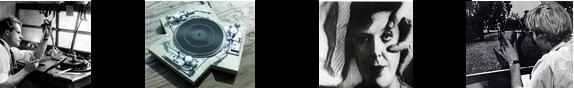
\includegraphics[width=\linewidth]{./TransdResearch/VRF-fig2.jpg}
%   \mycaption{ xxx )}\label{fig:profxxx}
   \end{center}
\end{figure}


The research group focuses on the study of four key aspects of visual competence: visual production competence, visual perception competence, visual reception competence, and multimodal/intercultural action competence. The research groups' logo - four images presented above - are symbolizing these four competences. The images are from left to right. (1) Analog film editing (production competence, anonymous source), (2) Sean Duffy, Thank You Ernest, JoJo \& Leslie, 2003 (multimodal action competence), (3) Filmstill from Luis Bu�uel, Un Chien Andalou, 1929 (perception competence), (4) Filmstill Michelangelo Antonioni, Blow Up, 1966 (reception competence).

\vspace{0.6cm}
A specific research project in the context of the Visual Research Focus "Visual Competence" is "Perceiving Press Photography: Who Sees What, When, How?" conducted by psychologists Prof. Bettina Olk and Prof. Arvid Kappas and mass communication Prof. Marion G. M�ller. In this transdisciplinary project, the perception, meaning attribution and reception of press photographs are tested in order to find out, how individuals, but also how different groups of participants (different gender, different social, national and cultural background) perceive and interpret contemporary news photographs depicting or relating to violent world events, and how they emotionally react to the same images.

\vspace{0.6cm}
IUB-members of Visual Competence research group (in alphabetical order): Profs. M. Bogaards, P. Crowther, J. F�rster, A. Kappas, U. K�hnen, P. Ludes, M. G. M�ller, B. Olk, H. Wessler, A. Wilhelm.

\vspace{0.6cm}
External invitees to the Visual Competence symposium and potential advisors and members of the Visual Competence research group (in order of appearance in the program): Profs. P. Messaris (University of Pennsylvania, Annenberg School, USA), J. Elkins (School of the Art Institute Chicago, USA), R. Hobbs (Temple University, USA), G. Kress (University of London, UK), M. Griffin (Carleton College, USA), K. Ritzenhoff (Central Connecticut State University, USA), T. Knieper (Ludwig Maximilians Universit�t M�nchen), H. Bredekamp (Humboldt-Universit�t zu Berlin), A. Kingstone (University of British Columbia in Vancouver, Canada), D. Glaser (The Wellcome Trust, UK), E. Tan (Universiteit van Amsterdam, Netherlands), F. Schwab/D. Unz (Universit�t Saarbr�cken), K. Holmqvist/J. Holsanova (University Lund, Sweden), T. van Leeuwen (University of Technology, Sydney, Australia), W. N�th (Universit�t Kassel), D. Freedberg (Columbia University, USA), L. Boccia (Federal University of Bahia, Salvador, Brazil), U. Frohne (Universit�t K�ln), B. Zelizer (University of Pennsylvania, Annenberg School, USA), M. Kraidy (American University, Washington D.C.), L. Santaella Braga (Catholic University of Sao Paulo, Brazil), M. Bruhn (Helmholtz-Zentrum, Berlin), C. M. Wolf (Universit�t Innsbruck, Austria), E. Grittmann (Universit�t Hamburg), B. Drechsel (Ludwig Boltzmann Institute for European History and Public Spheres, Gie�en), S. Baringhorst (Universit�t Siegen).


\newpage
\section{Completed Doctoral Degrees}
\shorttitle{Completed Doctoral Degrees}
\section{PhD Degrees}
\shorttitle{PhD Degrees}

\paragraph{2006} D\"orner, Jessica: ``A Self-Concept Measure of Personality Growth: Self-Concept Maturity (SCM). Development, Validation, and Age Effects''

Dissertation Committee: Prof. Dr. Ursula M. Staudinger (supervisor, IUB), Prof. Dr. Alexandra Freund (University of Zurich), Prof. Dr. Manfred Diehl (University of Florida, USA), Prof. Dr. Ulrich K\"uhnen (IUB), Prof. Dr. Britta Renner (IUB)

\paragraph{2006} Kessler, Eva-Marie: ``Intergenerational Relations as Facilitative Developmental Context'' 

Dissertation Committee: Prof. Dr. Ursula M. Staudinger (supervisor, IUB), Prof. Dr. Ute Kunzmann (IUB), Prof. Dr. Werner Greve (University of Hildesheim), Prof. Dr. Klaus Boehnke (IUB)

\paragraph{2005} Mickler, Charlotte: ``Self-related wisdom: Validation and age effects of a new measure of personal maturity'' 

Dissertation Committee: Prof. Dr. Ursula M. Staudinger (supervisor, IUB), Prof. Dr. Ute Kunzmann (IUB), Prof. Dr. Sigrun-Heide Filipp (University of Trier), Prof. Dr. Margrit Schreier (IUB)





\newpage
\section{Advisory Board}
\shorttitle{Advisory Board}

Prof. Dr. Bertrand Badie\newline
Professor of Political Science, Institut d'Etudes Politiques de Paris, France\\


Prof. Dr. Wim Blockmans\newline
Dean of the Arts Faculty, Leiden University, Netherlands\newline
Professor in Medieval History, Leiden University, Netherlands\\


Prof. Dr. Robert Erikson\newline
Professor of Sociology, Swedish Institute for Social Research, Stockholm University, Sweden\newline
Secretary General, Swedish Council for Working Life and Social Research\\


Prof. Dr. Erika Fischer-Lichte\newline
Director of the Institute of Theatre Studies at the Freie Universit�t Berlin\newline
President of the International Federation of Theatre Research\\


Prof. Dr. Kenneth Newton\newline
Professor of Comparative Politics, University of Southampton, England\\


Prof. Dr. Wolfgang Prinz\newline
Director, Max Planck Institute for Psychological Research, M�nchen\\


Prof. Dr. Wolfgang Schieder\newline
Professor Emeritus of History, Universit�t K�ln\\


Prof. Dr. Fritz Strack\newline
Professor of Psychology, Universit�t W�rzburg


\newpage
\section{Administration}
\shorttitle{Administration}
Prof. Dr. Hendrik Birus (Vice President and Dean)\\[-0.25cm] 

Dr. Freia Hardt (Director, Dean's Office)\\[-0.25cm]

Iris Krimmel (Director, Dean's Office)\\[-0.25cm]

Claire Freeman (Assistant to the Dean)\\[-0.25cm]

Iris Buck (Graduate Admission)\\[-0.25cm]

Bianca Bergmann (Team Assistant to the Faculty)\\[-0.25cm]

Rena Dickel (Team Assistant to the Faculty)\\[-0.25cm]

Kristine Hermann (Team Assistant European Utility Management)\\[-0.25cm]

Debora Jeske (Project Manager Sfb)\\[-0.25cm]

Dirk Schulte am H�lse (Laboratory Manager)\\[-0.25cm]



\newpage
\shorttitle{}


\newpage
\fchapter{}
\thispagestyle{empty}
%\begin{titlepage}
\vfil\null
}
\bigskip \bigskip \bigskip
\vspace{4.5in}
\large
{\bf Impressum}

Executive Editor:\\
Prof. Dr. Hendrik Birus\\
Dean of Humanities and Social Sciences\\

Editors:\\
Prof. Dr. Klaus Boehnke (Social Science Methodology)\\
Dr. Freia Hardt (Director, Office of the Dean)\\

Production Editors:\\
Bianca Bergmann (Team Assistant to the Faculty)\\
Rena Dickel (Team Assistant to the Faculty)\\
Silke Oberschachtsiek (Production, Corporate Communications and Media Relations)\\

Photos:\\
See references\\

\normalsize
\vfil\null
%\end{titlepage}




\end {document}
